\documentclass[11pt]{article}
\usepackage[margin=1in]{geometry}
\usepackage{enumitem}
\usepackage{hyperref}
\usepackage{graphicx}
\usepackage{array}
\usepackage{multicol}
\usepackage{longtable}
\usepackage{titlesec}
\usepackage{booktabs}
\usepackage{amsmath}
\usepackage{float}
\usepackage{sectsty}
\sectionfont{\fontsize{14}{16}\selectfont}
\subsectionfont{\fontsize{12}{14}\selectfont}

\documentclass[11pt]{article}

    \usepackage[breakable]{tcolorbox}
    \usepackage{parskip} % Stop auto-indenting (to mimic markdown behaviour)
    

    % Basic figure setup, for now with no caption control since it's done
    % automatically by Pandoc (which extracts ![](path) syntax from Markdown).
    \usepackage{graphicx}
    % Keep aspect ratio if custom image width or height is specified
    \setkeys{Gin}{keepaspectratio}
    % Maintain compatibility with old templates. Remove in nbconvert 6.0
    \let\Oldincludegraphics\includegraphics
    % Ensure that by default, figures have no caption (until we provide a
    % proper Figure object with a Caption API and a way to capture that
    % in the conversion process - todo).
    \usepackage{caption}
    \usepackage{float}
    \floatplacement{figure}{H} % forces figures to be placed at the correct location
    \usepackage{xcolor} % Allow colors to be defined
    \usepackage{enumerate} % Needed for markdown enumerations to work
    \usepackage{geometry} % Used to adjust the document margins
    \usepackage{amsmath} % Equations
    \usepackage{amssymb} % Equations
    \usepackage{textcomp} % defines textquotesingle
    % Hack from http://tex.stackexchange.com/a/47451/13684:
    \AtBeginDocument{%
        \def\PYZsq{\textquotesingle}% Upright quotes in Pygmentized code
    }
    \usepackage{upquote} % Upright quotes for verbatim code
    \usepackage{eurosym} % defines \euro

    \usepackage{iftex}
    \ifPDFTeX
        \usepackage[T1]{fontenc}
        \IfFileExists{alphabeta.sty}{
              \usepackage{alphabeta}
          }{
              \usepackage[mathletters]{ucs}
              \usepackage[utf8x]{inputenc}
          }
    \else
        \usepackage{fontspec}
        \usepackage{unicode-math}
    \fi

    \usepackage{fancyvrb} % verbatim replacement that allows latex
    \usepackage{grffile} % extends the file name processing of package graphics
                         % to support a larger range
    \makeatletter % fix for old versions of grffile with XeLaTeX
    \@ifpackagelater{grffile}{2019/11/01}
    {
      % Do nothing on new versions
    }
    {
      \def\Gread@@xetex#1{%
        \IfFileExists{"\Gin@base".bb}%
        {\Gread@eps{\Gin@base.bb}}%
        {\Gread@@xetex@aux#1}%
      }
    }
    \makeatother
    \usepackage[Export]{adjustbox} % Used to constrain images to a maximum size
    \adjustboxset{max size={0.9\linewidth}{0.9\paperheight}}

    % The hyperref package gives us a pdf with properly built
    % internal navigation ('pdf bookmarks' for the table of contents,
    % internal cross-reference links, web links for URLs, etc.)
    \usepackage{hyperref}
    % The default LaTeX title has an obnoxious amount of whitespace. By default,
    % titling removes some of it. It also provides customization options.
    \usepackage{titling}
    \usepackage{longtable} % longtable support required by pandoc >1.10
    \usepackage{booktabs}  % table support for pandoc > 1.12.2
    \usepackage{array}     % table support for pandoc >= 2.11.3
    \usepackage{calc}      % table minipage width calculation for pandoc >= 2.11.1
    \usepackage[inline]{enumitem} % IRkernel/repr support (it uses the enumerate* environment)
    \usepackage[normalem]{ulem} % ulem is needed to support strikethroughs (\sout)
                                % normalem makes italics be italics, not underlines
    \usepackage{soul}      % strikethrough (\st) support for pandoc >= 3.0.0
    \usepackage{mathrsfs}
    

    
    % Colors for the hyperref package
    \definecolor{urlcolor}{rgb}{0,.145,.698}
    \definecolor{linkcolor}{rgb}{.71,0.21,0.01}
    \definecolor{citecolor}{rgb}{.12,.54,.11}

    % ANSI colors
    \definecolor{ansi-black}{HTML}{3E424D}
    \definecolor{ansi-black-intense}{HTML}{282C36}
    \definecolor{ansi-red}{HTML}{E75C58}
    \definecolor{ansi-red-intense}{HTML}{B22B31}
    \definecolor{ansi-green}{HTML}{00A250}
    \definecolor{ansi-green-intense}{HTML}{007427}
    \definecolor{ansi-yellow}{HTML}{DDB62B}
    \definecolor{ansi-yellow-intense}{HTML}{B27D12}
    \definecolor{ansi-blue}{HTML}{208FFB}
    \definecolor{ansi-blue-intense}{HTML}{0065CA}
    \definecolor{ansi-magenta}{HTML}{D160C4}
    \definecolor{ansi-magenta-intense}{HTML}{A03196}
    \definecolor{ansi-cyan}{HTML}{60C6C8}
    \definecolor{ansi-cyan-intense}{HTML}{258F8F}
    \definecolor{ansi-white}{HTML}{C5C1B4}
    \definecolor{ansi-white-intense}{HTML}{A1A6B2}
    \definecolor{ansi-default-inverse-fg}{HTML}{FFFFFF}
    \definecolor{ansi-default-inverse-bg}{HTML}{000000}

    % common color for the border for error outputs.
    \definecolor{outerrorbackground}{HTML}{FFDFDF}

    % commands and environments needed by pandoc snippets
    % extracted from the output of `pandoc -s`
    \providecommand{\tightlist}{%
      \setlength{\itemsep}{0pt}\setlength{\parskip}{0pt}}
    \DefineVerbatimEnvironment{Highlighting}{Verbatim}{commandchars=\\\{\}}
    % Add ',fontsize=\small' for more characters per line
    \newenvironment{Shaded}{}{}
    \newcommand{\KeywordTok}[1]{\textcolor[rgb]{0.00,0.44,0.13}{\textbf{{#1}}}}
    \newcommand{\DataTypeTok}[1]{\textcolor[rgb]{0.56,0.13,0.00}{{#1}}}
    \newcommand{\DecValTok}[1]{\textcolor[rgb]{0.25,0.63,0.44}{{#1}}}
    \newcommand{\BaseNTok}[1]{\textcolor[rgb]{0.25,0.63,0.44}{{#1}}}
    \newcommand{\FloatTok}[1]{\textcolor[rgb]{0.25,0.63,0.44}{{#1}}}
    \newcommand{\CharTok}[1]{\textcolor[rgb]{0.25,0.44,0.63}{{#1}}}
    \newcommand{\StringTok}[1]{\textcolor[rgb]{0.25,0.44,0.63}{{#1}}}
    \newcommand{\CommentTok}[1]{\textcolor[rgb]{0.38,0.63,0.69}{\textit{{#1}}}}
    \newcommand{\OtherTok}[1]{\textcolor[rgb]{0.00,0.44,0.13}{{#1}}}
    \newcommand{\AlertTok}[1]{\textcolor[rgb]{1.00,0.00,0.00}{\textbf{{#1}}}}
    \newcommand{\FunctionTok}[1]{\textcolor[rgb]{0.02,0.16,0.49}{{#1}}}
    \newcommand{\RegionMarkerTok}[1]{{#1}}
    \newcommand{\ErrorTok}[1]{\textcolor[rgb]{1.00,0.00,0.00}{\textbf{{#1}}}}
    \newcommand{\NormalTok}[1]{{#1}}

    % Additional commands for more recent versions of Pandoc
    \newcommand{\ConstantTok}[1]{\textcolor[rgb]{0.53,0.00,0.00}{{#1}}}
    \newcommand{\SpecialCharTok}[1]{\textcolor[rgb]{0.25,0.44,0.63}{{#1}}}
    \newcommand{\VerbatimStringTok}[1]{\textcolor[rgb]{0.25,0.44,0.63}{{#1}}}
    \newcommand{\SpecialStringTok}[1]{\textcolor[rgb]{0.73,0.40,0.53}{{#1}}}
    \newcommand{\ImportTok}[1]{{#1}}
    \newcommand{\DocumentationTok}[1]{\textcolor[rgb]{0.73,0.13,0.13}{\textit{{#1}}}}
    \newcommand{\AnnotationTok}[1]{\textcolor[rgb]{0.38,0.63,0.69}{\textbf{\textit{{#1}}}}}
    \newcommand{\CommentVarTok}[1]{\textcolor[rgb]{0.38,0.63,0.69}{\textbf{\textit{{#1}}}}}
    \newcommand{\VariableTok}[1]{\textcolor[rgb]{0.10,0.09,0.49}{{#1}}}
    \newcommand{\ControlFlowTok}[1]{\textcolor[rgb]{0.00,0.44,0.13}{\textbf{{#1}}}}
    \newcommand{\OperatorTok}[1]{\textcolor[rgb]{0.40,0.40,0.40}{{#1}}}
    \newcommand{\BuiltInTok}[1]{{#1}}
    \newcommand{\ExtensionTok}[1]{{#1}}
    \newcommand{\PreprocessorTok}[1]{\textcolor[rgb]{0.74,0.48,0.00}{{#1}}}
    \newcommand{\AttributeTok}[1]{\textcolor[rgb]{0.49,0.56,0.16}{{#1}}}
    \newcommand{\InformationTok}[1]{\textcolor[rgb]{0.38,0.63,0.69}{\textbf{\textit{{#1}}}}}
    \newcommand{\WarningTok}[1]{\textcolor[rgb]{0.38,0.63,0.69}{\textbf{\textit{{#1}}}}}
    \makeatletter
    \newsavebox\pandoc@box
    \newcommand*\pandocbounded[1]{%
      \sbox\pandoc@box{#1}%
      % scaling factors for width and height
      \Gscale@div\@tempa\textheight{\dimexpr\ht\pandoc@box+\dp\pandoc@box\relax}%
      \Gscale@div\@tempb\linewidth{\wd\pandoc@box}%
      % select the smaller of both
      \ifdim\@tempb\p@<\@tempa\p@
        \let\@tempa\@tempb
      \fi
      % scaling accordingly (\@tempa < 1)
      \ifdim\@tempa\p@<\p@
        \scalebox{\@tempa}{\usebox\pandoc@box}%
      % scaling not needed, use as it is
      \else
        \usebox{\pandoc@box}%
      \fi
    }
    \makeatother

    % Define a nice break command that doesn't care if a line doesn't already
    % exist.
    \def\br{\hspace*{\fill} \\* }
    % Math Jax compatibility definitions
    \def\gt{>}
    \def\lt{<}
    \let\Oldtex\TeX
    \let\Oldlatex\LaTeX
    \renewcommand{\TeX}{\textrm{\Oldtex}}
    \renewcommand{\LaTeX}{\textrm{\Oldlatex}}
    % Document parameters
    % Document title
    \title{expt-6}
    
    
    
    
    
    
    
% Pygments definitions
\makeatletter
\def\PY@reset{\let\PY@it=\relax \let\PY@bf=\relax%
    \let\PY@ul=\relax \let\PY@tc=\relax%
    \let\PY@bc=\relax \let\PY@ff=\relax}
\def\PY@tok#1{\csname PY@tok@#1\endcsname}
\def\PY@toks#1+{\ifx\relax#1\empty\else%
    \PY@tok{#1}\expandafter\PY@toks\fi}
\def\PY@do#1{\PY@bc{\PY@tc{\PY@ul{%
    \PY@it{\PY@bf{\PY@ff{#1}}}}}}}
\def\PY#1#2{\PY@reset\PY@toks#1+\relax+\PY@do{#2}}

\@namedef{PY@tok@w}{\def\PY@tc##1{\textcolor[rgb]{0.73,0.73,0.73}{##1}}}
\@namedef{PY@tok@c}{\let\PY@it=\textit\def\PY@tc##1{\textcolor[rgb]{0.24,0.48,0.48}{##1}}}
\@namedef{PY@tok@cp}{\def\PY@tc##1{\textcolor[rgb]{0.61,0.40,0.00}{##1}}}
\@namedef{PY@tok@k}{\let\PY@bf=\textbf\def\PY@tc##1{\textcolor[rgb]{0.00,0.50,0.00}{##1}}}
\@namedef{PY@tok@kp}{\def\PY@tc##1{\textcolor[rgb]{0.00,0.50,0.00}{##1}}}
\@namedef{PY@tok@kt}{\def\PY@tc##1{\textcolor[rgb]{0.69,0.00,0.25}{##1}}}
\@namedef{PY@tok@o}{\def\PY@tc##1{\textcolor[rgb]{0.40,0.40,0.40}{##1}}}
\@namedef{PY@tok@ow}{\let\PY@bf=\textbf\def\PY@tc##1{\textcolor[rgb]{0.67,0.13,1.00}{##1}}}
\@namedef{PY@tok@nb}{\def\PY@tc##1{\textcolor[rgb]{0.00,0.50,0.00}{##1}}}
\@namedef{PY@tok@nf}{\def\PY@tc##1{\textcolor[rgb]{0.00,0.00,1.00}{##1}}}
\@namedef{PY@tok@nc}{\let\PY@bf=\textbf\def\PY@tc##1{\textcolor[rgb]{0.00,0.00,1.00}{##1}}}
\@namedef{PY@tok@nn}{\let\PY@bf=\textbf\def\PY@tc##1{\textcolor[rgb]{0.00,0.00,1.00}{##1}}}
\@namedef{PY@tok@ne}{\let\PY@bf=\textbf\def\PY@tc##1{\textcolor[rgb]{0.80,0.25,0.22}{##1}}}
\@namedef{PY@tok@nv}{\def\PY@tc##1{\textcolor[rgb]{0.10,0.09,0.49}{##1}}}
\@namedef{PY@tok@no}{\def\PY@tc##1{\textcolor[rgb]{0.53,0.00,0.00}{##1}}}
\@namedef{PY@tok@nl}{\def\PY@tc##1{\textcolor[rgb]{0.46,0.46,0.00}{##1}}}
\@namedef{PY@tok@ni}{\let\PY@bf=\textbf\def\PY@tc##1{\textcolor[rgb]{0.44,0.44,0.44}{##1}}}
\@namedef{PY@tok@na}{\def\PY@tc##1{\textcolor[rgb]{0.41,0.47,0.13}{##1}}}
\@namedef{PY@tok@nt}{\let\PY@bf=\textbf\def\PY@tc##1{\textcolor[rgb]{0.00,0.50,0.00}{##1}}}
\@namedef{PY@tok@nd}{\def\PY@tc##1{\textcolor[rgb]{0.67,0.13,1.00}{##1}}}
\@namedef{PY@tok@s}{\def\PY@tc##1{\textcolor[rgb]{0.73,0.13,0.13}{##1}}}
\@namedef{PY@tok@sd}{\let\PY@it=\textit\def\PY@tc##1{\textcolor[rgb]{0.73,0.13,0.13}{##1}}}
\@namedef{PY@tok@si}{\let\PY@bf=\textbf\def\PY@tc##1{\textcolor[rgb]{0.64,0.35,0.47}{##1}}}
\@namedef{PY@tok@se}{\let\PY@bf=\textbf\def\PY@tc##1{\textcolor[rgb]{0.67,0.36,0.12}{##1}}}
\@namedef{PY@tok@sr}{\def\PY@tc##1{\textcolor[rgb]{0.64,0.35,0.47}{##1}}}
\@namedef{PY@tok@ss}{\def\PY@tc##1{\textcolor[rgb]{0.10,0.09,0.49}{##1}}}
\@namedef{PY@tok@sx}{\def\PY@tc##1{\textcolor[rgb]{0.00,0.50,0.00}{##1}}}
\@namedef{PY@tok@m}{\def\PY@tc##1{\textcolor[rgb]{0.40,0.40,0.40}{##1}}}
\@namedef{PY@tok@gh}{\let\PY@bf=\textbf\def\PY@tc##1{\textcolor[rgb]{0.00,0.00,0.50}{##1}}}
\@namedef{PY@tok@gu}{\let\PY@bf=\textbf\def\PY@tc##1{\textcolor[rgb]{0.50,0.00,0.50}{##1}}}
\@namedef{PY@tok@gd}{\def\PY@tc##1{\textcolor[rgb]{0.63,0.00,0.00}{##1}}}
\@namedef{PY@tok@gi}{\def\PY@tc##1{\textcolor[rgb]{0.00,0.52,0.00}{##1}}}
\@namedef{PY@tok@gr}{\def\PY@tc##1{\textcolor[rgb]{0.89,0.00,0.00}{##1}}}
\@namedef{PY@tok@ge}{\let\PY@it=\textit}
\@namedef{PY@tok@gs}{\let\PY@bf=\textbf}
\@namedef{PY@tok@ges}{\let\PY@bf=\textbf\let\PY@it=\textit}
\@namedef{PY@tok@gp}{\let\PY@bf=\textbf\def\PY@tc##1{\textcolor[rgb]{0.00,0.00,0.50}{##1}}}
\@namedef{PY@tok@go}{\def\PY@tc##1{\textcolor[rgb]{0.44,0.44,0.44}{##1}}}
\@namedef{PY@tok@gt}{\def\PY@tc##1{\textcolor[rgb]{0.00,0.27,0.87}{##1}}}
\@namedef{PY@tok@err}{\def\PY@bc##1{{\setlength{\fboxsep}{\string -\fboxrule}\fcolorbox[rgb]{1.00,0.00,0.00}{1,1,1}{\strut ##1}}}}
\@namedef{PY@tok@kc}{\let\PY@bf=\textbf\def\PY@tc##1{\textcolor[rgb]{0.00,0.50,0.00}{##1}}}
\@namedef{PY@tok@kd}{\let\PY@bf=\textbf\def\PY@tc##1{\textcolor[rgb]{0.00,0.50,0.00}{##1}}}
\@namedef{PY@tok@kn}{\let\PY@bf=\textbf\def\PY@tc##1{\textcolor[rgb]{0.00,0.50,0.00}{##1}}}
\@namedef{PY@tok@kr}{\let\PY@bf=\textbf\def\PY@tc##1{\textcolor[rgb]{0.00,0.50,0.00}{##1}}}
\@namedef{PY@tok@bp}{\def\PY@tc##1{\textcolor[rgb]{0.00,0.50,0.00}{##1}}}
\@namedef{PY@tok@fm}{\def\PY@tc##1{\textcolor[rgb]{0.00,0.00,1.00}{##1}}}
\@namedef{PY@tok@vc}{\def\PY@tc##1{\textcolor[rgb]{0.10,0.09,0.49}{##1}}}
\@namedef{PY@tok@vg}{\def\PY@tc##1{\textcolor[rgb]{0.10,0.09,0.49}{##1}}}
\@namedef{PY@tok@vi}{\def\PY@tc##1{\textcolor[rgb]{0.10,0.09,0.49}{##1}}}
\@namedef{PY@tok@vm}{\def\PY@tc##1{\textcolor[rgb]{0.10,0.09,0.49}{##1}}}
\@namedef{PY@tok@sa}{\def\PY@tc##1{\textcolor[rgb]{0.73,0.13,0.13}{##1}}}
\@namedef{PY@tok@sb}{\def\PY@tc##1{\textcolor[rgb]{0.73,0.13,0.13}{##1}}}
\@namedef{PY@tok@sc}{\def\PY@tc##1{\textcolor[rgb]{0.73,0.13,0.13}{##1}}}
\@namedef{PY@tok@dl}{\def\PY@tc##1{\textcolor[rgb]{0.73,0.13,0.13}{##1}}}
\@namedef{PY@tok@s2}{\def\PY@tc##1{\textcolor[rgb]{0.73,0.13,0.13}{##1}}}
\@namedef{PY@tok@sh}{\def\PY@tc##1{\textcolor[rgb]{0.73,0.13,0.13}{##1}}}
\@namedef{PY@tok@s1}{\def\PY@tc##1{\textcolor[rgb]{0.73,0.13,0.13}{##1}}}
\@namedef{PY@tok@mb}{\def\PY@tc##1{\textcolor[rgb]{0.40,0.40,0.40}{##1}}}
\@namedef{PY@tok@mf}{\def\PY@tc##1{\textcolor[rgb]{0.40,0.40,0.40}{##1}}}
\@namedef{PY@tok@mh}{\def\PY@tc##1{\textcolor[rgb]{0.40,0.40,0.40}{##1}}}
\@namedef{PY@tok@mi}{\def\PY@tc##1{\textcolor[rgb]{0.40,0.40,0.40}{##1}}}
\@namedef{PY@tok@il}{\def\PY@tc##1{\textcolor[rgb]{0.40,0.40,0.40}{##1}}}
\@namedef{PY@tok@mo}{\def\PY@tc##1{\textcolor[rgb]{0.40,0.40,0.40}{##1}}}
\@namedef{PY@tok@ch}{\let\PY@it=\textit\def\PY@tc##1{\textcolor[rgb]{0.24,0.48,0.48}{##1}}}
\@namedef{PY@tok@cm}{\let\PY@it=\textit\def\PY@tc##1{\textcolor[rgb]{0.24,0.48,0.48}{##1}}}
\@namedef{PY@tok@cpf}{\let\PY@it=\textit\def\PY@tc##1{\textcolor[rgb]{0.24,0.48,0.48}{##1}}}
\@namedef{PY@tok@c1}{\let\PY@it=\textit\def\PY@tc##1{\textcolor[rgb]{0.24,0.48,0.48}{##1}}}
\@namedef{PY@tok@cs}{\let\PY@it=\textit\def\PY@tc##1{\textcolor[rgb]{0.24,0.48,0.48}{##1}}}

\def\PYZbs{\char`\\}
\def\PYZus{\char`\_}
\def\PYZob{\char`\{}
\def\PYZcb{\char`\}}
\def\PYZca{\char`\^}
\def\PYZam{\char`\&}
\def\PYZlt{\char`\<}
\def\PYZgt{\char`\>}
\def\PYZsh{\char`\#}
\def\PYZpc{\char`\%}
\def\PYZdl{\char`\$}
\def\PYZhy{\char`\-}
\def\PYZsq{\char`\'}
\def\PYZdq{\char`\"}
\def\PYZti{\char`\~}
% for compatibility with earlier versions
\def\PYZat{@}
\def\PYZlb{[}
\def\PYZrb{]}
\makeatother


    % For linebreaks inside Verbatim environment from package fancyvrb.
    \makeatletter
        \newbox\Wrappedcontinuationbox
        \newbox\Wrappedvisiblespacebox
        \newcommand*\Wrappedvisiblespace {\textcolor{red}{\textvisiblespace}}
        \newcommand*\Wrappedcontinuationsymbol {\textcolor{red}{\llap{\tiny$\m@th\hookrightarrow$}}}
        \newcommand*\Wrappedcontinuationindent {3ex }
        \newcommand*\Wrappedafterbreak {\kern\Wrappedcontinuationindent\copy\Wrappedcontinuationbox}
        % Take advantage of the already applied Pygments mark-up to insert
        % potential linebreaks for TeX processing.
        %        {, <, #, %, $, ' and ": go to next line.
        %        _, }, ^, &, >, - and ~: stay at end of broken line.
        % Use of \textquotesingle for straight quote.
        \newcommand*\Wrappedbreaksatspecials {%
            \def\PYGZus{\discretionary{\char`\_}{\Wrappedafterbreak}{\char`\_}}%
            \def\PYGZob{\discretionary{}{\Wrappedafterbreak\char`\{}{\char`\{}}%
            \def\PYGZcb{\discretionary{\char`\}}{\Wrappedafterbreak}{\char`\}}}%
            \def\PYGZca{\discretionary{\char`\^}{\Wrappedafterbreak}{\char`\^}}%
            \def\PYGZam{\discretionary{\char`\&}{\Wrappedafterbreak}{\char`\&}}%
            \def\PYGZlt{\discretionary{}{\Wrappedafterbreak\char`\<}{\char`\<}}%
            \def\PYGZgt{\discretionary{\char`\>}{\Wrappedafterbreak}{\char`\>}}%
            \def\PYGZsh{\discretionary{}{\Wrappedafterbreak\char`\#}{\char`\#}}%
            \def\PYGZpc{\discretionary{}{\Wrappedafterbreak\char`\%}{\char`\%}}%
            \def\PYGZdl{\discretionary{}{\Wrappedafterbreak\char`\$}{\char`\$}}%
            \def\PYGZhy{\discretionary{\char`\-}{\Wrappedafterbreak}{\char`\-}}%
            \def\PYGZsq{\discretionary{}{\Wrappedafterbreak\textquotesingle}{\textquotesingle}}%
            \def\PYGZdq{\discretionary{}{\Wrappedafterbreak\char`\"}{\char`\"}}%
            \def\PYGZti{\discretionary{\char`\~}{\Wrappedafterbreak}{\char`\~}}%
        }
        % Some characters . , ; ? ! / are not pygmentized.
        % This macro makes them "active" and they will insert potential linebreaks
        \newcommand*\Wrappedbreaksatpunct {%
            \lccode`\~`\.\lowercase{\def~}{\discretionary{\hbox{\char`\.}}{\Wrappedafterbreak}{\hbox{\char`\.}}}%
            \lccode`\~`\,\lowercase{\def~}{\discretionary{\hbox{\char`\,}}{\Wrappedafterbreak}{\hbox{\char`\,}}}%
            \lccode`\~`\;\lowercase{\def~}{\discretionary{\hbox{\char`\;}}{\Wrappedafterbreak}{\hbox{\char`\;}}}%
            \lccode`\~`\:\lowercase{\def~}{\discretionary{\hbox{\char`\:}}{\Wrappedafterbreak}{\hbox{\char`\:}}}%
            \lccode`\~`\?\lowercase{\def~}{\discretionary{\hbox{\char`\?}}{\Wrappedafterbreak}{\hbox{\char`\?}}}%
            \lccode`\~`\!\lowercase{\def~}{\discretionary{\hbox{\char`\!}}{\Wrappedafterbreak}{\hbox{\char`\!}}}%
            \lccode`\~`\/\lowercase{\def~}{\discretionary{\hbox{\char`\/}}{\Wrappedafterbreak}{\hbox{\char`\/}}}%
            \catcode`\.\active
            \catcode`\,\active
            \catcode`\;\active
            \catcode`\:\active
            \catcode`\?\active
            \catcode`\!\active
            \catcode`\/\active
            \lccode`\~`\~
        }
    \makeatother

    \let\OriginalVerbatim=\Verbatim
    \makeatletter
    \renewcommand{\Verbatim}[1][1]{%
        %\parskip\z@skip
        \sbox\Wrappedcontinuationbox {\Wrappedcontinuationsymbol}%
        \sbox\Wrappedvisiblespacebox {\FV@SetupFont\Wrappedvisiblespace}%
        \def\FancyVerbFormatLine ##1{\hsize\linewidth
            \vtop{\raggedright\hyphenpenalty\z@\exhyphenpenalty\z@
                \doublehyphendemerits\z@\finalhyphendemerits\z@
                \strut ##1\strut}%
        }%
        % If the linebreak is at a space, the latter will be displayed as visible
        % space at end of first line, and a continuation symbol starts next line.
        % Stretch/shrink are however usually zero for typewriter font.
        \def\FV@Space {%
            \nobreak\hskip\z@ plus\fontdimen3\font minus\fontdimen4\font
            \discretionary{\copy\Wrappedvisiblespacebox}{\Wrappedafterbreak}
            {\kern\fontdimen2\font}%
        }%

        % Allow breaks at special characters using \PYG... macros.
        \Wrappedbreaksatspecials
        % Breaks at punctuation characters . , ; ? ! and / need catcode=\active
        \OriginalVerbatim[#1,codes*=\Wrappedbreaksatpunct]%
    }
    \makeatother

    % Exact colors from NB
    \definecolor{incolor}{HTML}{303F9F}
    \definecolor{outcolor}{HTML}{D84315}
    \definecolor{cellborder}{HTML}{CFCFCF}
    \definecolor{cellbackground}{HTML}{F7F7F7}

    % prompt
    \makeatletter
    \newcommand{\boxspacing}{\kern\kvtcb@left@rule\kern\kvtcb@boxsep}
    \makeatother
    \newcommand{\prompt}[4]{
        {\ttfamily\llap{{\color{#2}[#3]:\hspace{3pt}#4}}\vspace{-\baselineskip}}
    }
    

    
    % Prevent overflowing lines due to hard-to-break entities
    \sloppy
    % Setup hyperref package
    \hypersetup{
      breaklinks=true,  % so long urls are correctly broken across lines
      colorlinks=true,
      urlcolor=urlcolor,
      linkcolor=linkcolor,
      citecolor=citecolor,
      }
    % Slightly bigger margins than the latex defaults
    
    \geometry{verbose,tmargin=1in,bmargin=1in,lmargin=1in,rmargin=1in}
    
    

\begin{document}
    
    \begin{center}
    \large \textbf{Sri Sivasubramaniya Nadar College of Engineering, Chennai} \\
    (An autonomous Institution affiliated to Anna University) \\
    \vspace{0.3cm}
\end{center}

\begin{table}[!h]
\renewcommand{\arraystretch}{1.5}
\resizebox{\textwidth}{!}{%
\begin{tabular}{|l|cll|}
\hline
Degree \& Branch     & \multicolumn{1}{c|}{B.E. Computer Science \& Engineering} & \multicolumn{1}{l|}{Semester}        & V                                        \\ \hline
Subject Code \& Name & \multicolumn{3}{c|}{ICS1512 - Machine Learning Algorithms Laboratory}                                                                              \\ \hline
Academic year       & \multicolumn{1}{c|}{2025-2026 (Odd)}                        & \multicolumn{1}{c|}{Batch: 2023-2028} & \multicolumn{1}{c|}{\textbf{Due date: }} \\ \hline
\end{tabular}%
}
\end{table}

\vspace{0.5cm}

\begin{center}
 \textbf{Experiment 6: Dimensionality Reduction and Model
 Evaluation (With and Without PCA)}
\end{center}

\vspace{0.3cm}
\noindent
\section{Aim:} 
  To study the effect of dimensionality reduction using Principal Component Analysis (PCA) on the performance of various machine learning classifiers. The task requires:
 
 a) Training and validating models without PCA (original feature space).
 
 b) Training and validating models with PCA (reduced feature space).
 
 For both cases, students must perform hyperparameter tuning, apply 5-fold cross-validation, and record performance.

\vspace{0.3cm}
\noindent
\section{Libraries used:}
\begin{itemize}
    \item {Pandas}
    \item {Numpy}
    \item {Matplotlib}
    \item {Scikit-learn}
    \item {XGBoost}
\end{itemize}

\vspace{0.3cm}
\noindent
\section{Objective:} 
To evaluate how dimensionality reduction using Principal Component Analysis (PCA) influences the accuracy and generalization of different machine learning classifiers, by comparing their performance with and without PCA through hyperparameter tuning and 5-fold cross-validation. 

\vspace{0.6cm}
    \begin{tcolorbox}[breakable, size=fbox, boxrule=1pt, pad at break*=1mm,colback=cellbackground, colframe=cellborder]
\prompt{In}{incolor}{16}{\boxspacing}
\begin{Verbatim}[commandchars=\\\{\}]
\PY{n}{TARGET\PYZus{}COLUMN} \PY{o}{=} \PY{l+s+s1}{\PYZsq{}}\PY{l+s+s1}{class}\PY{l+s+s1}{\PYZsq{}}
\PY{n}{df} \PY{o}{=} \PY{n}{pd}\PY{o}{.}\PY{n}{read\PYZus{}csv}\PY{p}{(}\PY{l+s+s1}{\PYZsq{}}\PY{l+s+s1}{/content/drive/MyDrive/ml\PYZhy{}lab/spambase\PYZus{}csv.csv}\PY{l+s+s1}{\PYZsq{}}\PY{p}{)}
\PY{n+nb}{print}\PY{p}{(}\PY{n}{df}\PY{o}{.}\PY{n}{head}\PY{p}{(}\PY{p}{)}\PY{p}{)}
\PY{n+nb}{print}\PY{p}{(}\PY{l+s+s2}{\PYZdq{}}\PY{l+s+s2}{Initial shape:}\PY{l+s+s2}{\PYZdq{}}\PY{p}{,} \PY{n}{df}\PY{o}{.}\PY{n}{shape}\PY{p}{)}
\end{Verbatim}
\end{tcolorbox}

    \begin{Verbatim}[commandchars=\\\{\}]
   word\_freq\_make  word\_freq\_address  word\_freq\_all  word\_freq\_3d  \textbackslash{}
0            0.00               0.64           0.64           0.0
1            0.21               0.28           0.50           0.0
2            0.06               0.00           0.71           0.0
3            0.00               0.00           0.00           0.0
4            0.00               0.00           0.00           0.0

   word\_freq\_our  word\_freq\_over  word\_freq\_remove  word\_freq\_internet  \textbackslash{}
0           0.32            0.00              0.00                0.00
1           0.14            0.28              0.21                0.07
2           1.23            0.19              0.19                0.12
3           0.63            0.00              0.31                0.63
4           0.63            0.00              0.31                0.63

   word\_freq\_order  word\_freq\_mail  {\ldots}  char\_freq\_\%3B  char\_freq\_\%28  \textbackslash{}
0             0.00            0.00  {\ldots}           0.00          0.000
1             0.00            0.94  {\ldots}           0.00          0.132
2             0.64            0.25  {\ldots}           0.01          0.143
3             0.31            0.63  {\ldots}           0.00          0.137
4             0.31            0.63  {\ldots}           0.00          0.135

   char\_freq\_\%5B  char\_freq\_\%21  char\_freq\_\%24  char\_freq\_\%23  \textbackslash{}
0            0.0          0.778          0.000          0.000
1            0.0          0.372          0.180          0.048
2            0.0          0.276          0.184          0.010
3            0.0          0.137          0.000          0.000
4            0.0          0.135          0.000          0.000

   capital\_run\_length\_average  capital\_run\_length\_longest  \textbackslash{}
0                       3.756                          61
1                       5.114                         101
2                       9.821                         485
3                       3.537                          40
4                       3.537                          40

   capital\_run\_length\_total  class
0                       278      1
1                      1028      1
2                      2259      1
3                       191      1
4                       191      1

[5 rows x 58 columns]
Initial shape: (4601, 58)
    \end{Verbatim}
    
\vspace{0.6cm}
    \begin{tcolorbox}[breakable, size=fbox, boxrule=1pt, pad at break*=1mm,colback=cellbackground, colframe=cellborder]
\prompt{In}{incolor}{17}{\boxspacing}
\begin{Verbatim}[commandchars=\\\{\}]
\PY{c+c1}{\PYZsh{} HANDLE MISSING VALUES}
\PY{n}{df} \PY{o}{=} \PY{n}{df}\PY{o}{.}\PY{n}{dropna}\PY{p}{(}\PY{n}{thresh}\PY{o}{=}\PY{n}{df}\PY{o}{.}\PY{n}{shape}\PY{p}{[}\PY{l+m+mi}{1}\PY{p}{]}\PY{o}{/}\PY{o}{/}\PY{l+m+mi}{2}\PY{p}{)}  \PY{c+c1}{\PYZsh{} Drop rows with \PYZgt{}50\PYZpc{} missing}
\PY{n}{df}\PY{o}{.}\PY{n}{fillna}\PY{p}{(}\PY{n}{df}\PY{o}{.}\PY{n}{median}\PY{p}{(}\PY{n}{numeric\PYZus{}only}\PY{o}{=}\PY{k+kc}{True}\PY{p}{)}\PY{p}{,} \PY{n}{inplace}\PY{o}{=}\PY{k+kc}{True}\PY{p}{)}

\PY{c+c1}{\PYZsh{} OUTLIER HANDLING (Z\PYZhy{}Score)}
\PY{k}{def}\PY{+w}{ }\PY{n+nf}{remove\PYZus{}outliers}\PY{p}{(}\PY{n}{df}\PY{p}{,} \PY{n}{threshold}\PY{o}{=}\PY{l+m+mi}{3}\PY{p}{)}\PY{p}{:}
    \PY{n}{numeric\PYZus{}cols} \PY{o}{=} \PY{n}{df}\PY{o}{.}\PY{n}{select\PYZus{}dtypes}\PY{p}{(}\PY{n}{include}\PY{o}{=}\PY{p}{[}\PY{n}{np}\PY{o}{.}\PY{n}{number}\PY{p}{]}\PY{p}{)}\PY{o}{.}\PY{n}{columns}
    \PY{n}{z\PYZus{}scores} \PY{o}{=} \PY{n}{np}\PY{o}{.}\PY{n}{abs}\PY{p}{(}\PY{p}{(}\PY{n}{df}\PY{p}{[}\PY{n}{numeric\PYZus{}cols}\PY{p}{]} \PY{o}{\PYZhy{}} \PY{n}{df}\PY{p}{[}\PY{n}{numeric\PYZus{}cols}\PY{p}{]}\PY{o}{.}\PY{n}{mean}\PY{p}{(}\PY{p}{)}\PY{p}{)} \PY{o}{/} \PY{n}{df}\PY{p}{[}\PY{n}{numeric\PYZus{}cols}\PY{p}{]}\PY{o}{.}\PY{n}{std}\PY{p}{(}\PY{p}{)}\PY{p}{)}
    \PY{k}{return} \PY{n}{df}\PY{p}{[}\PY{p}{(}\PY{n}{z\PYZus{}scores} \PY{o}{\PYZlt{}} \PY{n}{threshold}\PY{p}{)}\PY{o}{.}\PY{n}{all}\PY{p}{(}\PY{n}{axis}\PY{o}{=}\PY{l+m+mi}{1}\PY{p}{)}\PY{p}{]}

\PY{n}{df} \PY{o}{=} \PY{n}{remove\PYZus{}outliers}\PY{p}{(}\PY{n}{df}\PY{p}{)}
\PY{c+c1}{\PYZsh{} print(\PYZdq{}After outlier removal:\PYZdq{}, df.shape)}
\end{Verbatim}
\end{tcolorbox}
\vspace{0.4cm}
    \begin{tcolorbox}[breakable, size=fbox, boxrule=1pt, pad at break*=1mm,colback=cellbackground, colframe=cellborder]
\prompt{In}{incolor}{18}{\boxspacing}
\begin{Verbatim}[commandchars=\\\{\}]
\PY{c+c1}{\PYZsh{} FEATURE / TARGET SPLIT}
\PY{n}{X} \PY{o}{=} \PY{n}{df}\PY{o}{.}\PY{n}{drop}\PY{p}{(}\PY{n}{columns}\PY{o}{=}\PY{p}{[}\PY{n}{TARGET\PYZus{}COLUMN}\PY{p}{]}\PY{p}{)}
\PY{n}{y} \PY{o}{=} \PY{n}{df}\PY{p}{[}\PY{n}{TARGET\PYZus{}COLUMN}\PY{p}{]}

\PY{c+c1}{\PYZsh{} ENCODE + STANDARDIZE}
\PY{n}{numeric\PYZus{}cols} \PY{o}{=} \PY{n}{X}\PY{o}{.}\PY{n}{select\PYZus{}dtypes}\PY{p}{(}\PY{n}{include}\PY{o}{=}\PY{p}{[}\PY{n}{np}\PY{o}{.}\PY{n}{number}\PY{p}{]}\PY{p}{)}\PY{o}{.}\PY{n}{columns}
\PY{n}{categorical\PYZus{}cols} \PY{o}{=} \PY{n}{X}\PY{o}{.}\PY{n}{select\PYZus{}dtypes}\PY{p}{(}\PY{n}{exclude}\PY{o}{=}\PY{p}{[}\PY{n}{np}\PY{o}{.}\PY{n}{number}\PY{p}{]}\PY{p}{)}\PY{o}{.}\PY{n}{columns}
\PY{n}{X\PYZus{}encoded} \PY{o}{=} \PY{n}{pd}\PY{o}{.}\PY{n}{get\PYZus{}dummies}\PY{p}{(}\PY{n}{X}\PY{p}{,} \PY{n}{columns}\PY{o}{=}\PY{n}{categorical\PYZus{}cols}\PY{p}{)}
\PY{n}{scaler} \PY{o}{=} \PY{n}{StandardScaler}\PY{p}{(}\PY{p}{)}
\PY{n}{X\PYZus{}scaled} \PY{o}{=} \PY{n}{scaler}\PY{o}{.}\PY{n}{fit\PYZus{}transform}\PY{p}{(}\PY{n}{X\PYZus{}encoded}\PY{p}{)}

\PY{c+c1}{\PYZsh{} TRAIN / TEST SPLIT}
\PY{n}{X\PYZus{}train}\PY{p}{,} \PY{n}{X\PYZus{}test}\PY{p}{,} \PY{n}{y\PYZus{}train}\PY{p}{,} \PY{n}{y\PYZus{}test} \PY{o}{=} \PY{n}{train\PYZus{}test\PYZus{}split}\PY{p}{(}
    \PY{n}{X\PYZus{}scaled}\PY{p}{,}
    \PY{n}{y}\PY{p}{,}
    \PY{n}{test\PYZus{}size}\PY{o}{=}\PY{l+m+mf}{0.2}\PY{p}{,}          \PY{c+c1}{\PYZsh{} 20\PYZpc{} test hold\PYZhy{}out}
    \PY{n}{stratify}\PY{o}{=}\PY{n}{y}\PY{p}{,}             \PY{c+c1}{\PYZsh{} keep class balance if classification}
    \PY{n}{random\PYZus{}state}\PY{o}{=}\PY{l+m+mi}{42}
\PY{p}{)}
\end{Verbatim}
\end{tcolorbox}

\vspace{0.6cm}
    \textbf{PCA Variance Explained}

    \begin{tcolorbox}[breakable, size=fbox, boxrule=1pt, pad at break*=1mm,colback=cellbackground, colframe=cellborder]
\prompt{In}{incolor}{39}{\boxspacing}
\begin{Verbatim}[commandchars=\\\{\}]
\PY{n}{pca} \PY{o}{=} \PY{n}{PCA}\PY{p}{(}\PY{n}{n\PYZus{}components}\PY{o}{=}\PY{l+m+mf}{0.95}\PY{p}{)}
\PY{n}{pca}\PY{o}{.}\PY{n}{fit}\PY{p}{(}\PY{n}{X\PYZus{}scaled}\PY{p}{)}

\PY{n+nb}{print}\PY{p}{(}\PY{l+s+s2}{\PYZdq{}}\PY{l+s+s2}{Chosen components:}\PY{l+s+s2}{\PYZdq{}}\PY{p}{,} \PY{n}{pca}\PY{o}{.}\PY{n}{n\PYZus{}components\PYZus{}}\PY{p}{)}
\PY{n+nb}{print}\PY{p}{(}\PY{l+s+s2}{\PYZdq{}}\PY{l+s+s2}{Total variance explained (}\PY{l+s+s2}{\PYZpc{}}\PY{l+s+s2}{):}\PY{l+s+s2}{\PYZdq{}}\PY{p}{,} \PY{n}{pca}\PY{o}{.}\PY{n}{explained\PYZus{}variance\PYZus{}ratio\PYZus{}}\PY{o}{.}\PY{n}{sum}\PY{p}{(}\PY{p}{)}\PY{o}{*}\PY{l+m+mi}{100}\PY{p}{)}
\end{Verbatim}
\end{tcolorbox}

    \begin{Verbatim}[commandchars=\\\{\}]
Chosen components: 49
Total variance explained (\%): 95.53617010131482
    \end{Verbatim}
    
\vspace{0.6cm}
    \textbf{Support Vector Machine (SVM)}

    \begin{tcolorbox}[breakable, size=fbox, boxrule=1pt, pad at break*=1mm,colback=cellbackground, colframe=cellborder]
\prompt{In}{incolor}{23}{\boxspacing}
\begin{Verbatim}[commandchars=\\\{\}]
\PY{c+c1}{\PYZsh{} ========== HYPERPARAM GRID ==========}
\PY{n}{param\PYZus{}grid} \PY{o}{=} \PY{p}{\PYZob{}}
    \PY{l+s+s1}{\PYZsq{}}\PY{l+s+s1}{kernel}\PY{l+s+s1}{\PYZsq{}}\PY{p}{:} \PY{p}{[}\PY{l+s+s1}{\PYZsq{}}\PY{l+s+s1}{linear}\PY{l+s+s1}{\PYZsq{}}\PY{p}{,} \PY{l+s+s1}{\PYZsq{}}\PY{l+s+s1}{rbf}\PY{l+s+s1}{\PYZsq{}}\PY{p}{]}\PY{p}{,}
    \PY{l+s+s1}{\PYZsq{}}\PY{l+s+s1}{C}\PY{l+s+s1}{\PYZsq{}}\PY{p}{:} \PY{p}{[}\PY{l+m+mf}{0.1}\PY{p}{,} \PY{l+m+mi}{10}\PY{p}{]}\PY{p}{,}
    \PY{l+s+s1}{\PYZsq{}}\PY{l+s+s1}{gamma}\PY{l+s+s1}{\PYZsq{}}\PY{p}{:} \PY{p}{[}\PY{l+s+s1}{\PYZsq{}}\PY{l+s+s1}{scale}\PY{l+s+s1}{\PYZsq{}}\PY{p}{]}
\PY{p}{\PYZcb{}}

\PY{c+c1}{\PYZsh{} ========== HELPER FUNCTION ==========}
\PY{k}{def}\PY{+w}{ }\PY{n+nf}{evaluate\PYZus{}svc}\PY{p}{(}\PY{n}{X\PYZus{}train}\PY{p}{,} \PY{n}{X\PYZus{}test}\PY{p}{,} \PY{n}{y\PYZus{}train}\PY{p}{,} \PY{n}{y\PYZus{}test}\PY{p}{,} \PY{n}{use\PYZus{}pca}\PY{o}{=}\PY{k+kc}{False}\PY{p}{,} \PY{n}{pca\PYZus{}variance}\PY{o}{=}\PY{l+m+mf}{0.95}\PY{p}{)}\PY{p}{:}
    \PY{k}{if} \PY{n}{use\PYZus{}pca}\PY{p}{:}
        \PY{n}{pca} \PY{o}{=} \PY{n}{PCA}\PY{p}{(}\PY{n}{n\PYZus{}components}\PY{o}{=}\PY{n}{pca\PYZus{}variance}\PY{p}{)}
        \PY{n}{X\PYZus{}train\PYZus{}proc} \PY{o}{=} \PY{n}{pca}\PY{o}{.}\PY{n}{fit\PYZus{}transform}\PY{p}{(}\PY{n}{X\PYZus{}train}\PY{p}{)}
        \PY{n}{X\PYZus{}test\PYZus{}proc} \PY{o}{=} \PY{n}{pca}\PY{o}{.}\PY{n}{transform}\PY{p}{(}\PY{n}{X\PYZus{}test}\PY{p}{)}
    \PY{k}{else}\PY{p}{:}
        \PY{n}{X\PYZus{}train\PYZus{}proc} \PY{o}{=} \PY{n}{X\PYZus{}train}
        \PY{n}{X\PYZus{}test\PYZus{}proc} \PY{o}{=} \PY{n}{X\PYZus{}test}

    \PY{n}{svc} \PY{o}{=} \PY{n}{SVC}\PY{p}{(}\PY{n}{probability}\PY{o}{=}\PY{k+kc}{True}\PY{p}{)}
    \PY{n}{grid} \PY{o}{=} \PY{n}{GridSearchCV}\PY{p}{(}\PY{n}{svc}\PY{p}{,} \PY{n}{param\PYZus{}grid}\PY{p}{,} \PY{n}{cv}\PY{o}{=}\PY{l+m+mi}{5}\PY{p}{,} \PY{n}{scoring}\PY{o}{=}\PY{l+s+s1}{\PYZsq{}}\PY{l+s+s1}{accuracy}\PY{l+s+s1}{\PYZsq{}}\PY{p}{)}  \PY{c+c1}{\PYZsh{} you can switch scoring}
    \PY{n}{grid}\PY{o}{.}\PY{n}{fit}\PY{p}{(}\PY{n}{X\PYZus{}train\PYZus{}proc}\PY{p}{,} \PY{n}{y\PYZus{}train}\PY{p}{)}

    \PY{n}{best\PYZus{}model} \PY{o}{=} \PY{n}{grid}\PY{o}{.}\PY{n}{best\PYZus{}estimator\PYZus{}}
    \PY{n}{y\PYZus{}pred} \PY{o}{=} \PY{n}{best\PYZus{}model}\PY{o}{.}\PY{n}{predict}\PY{p}{(}\PY{n}{X\PYZus{}test\PYZus{}proc}\PY{p}{)}
    \PY{n}{y\PYZus{}proba} \PY{o}{=} \PY{n}{best\PYZus{}model}\PY{o}{.}\PY{n}{predict\PYZus{}proba}\PY{p}{(}\PY{n}{X\PYZus{}test\PYZus{}proc}\PY{p}{)}\PY{p}{[}\PY{p}{:}\PY{p}{,}\PY{l+m+mi}{1}\PY{p}{]}

    \PY{n}{acc} \PY{o}{=} \PY{n}{accuracy\PYZus{}score}\PY{p}{(}\PY{n}{y\PYZus{}test}\PY{p}{,} \PY{n}{y\PYZus{}pred}\PY{p}{)}
    \PY{n}{auc} \PY{o}{=} \PY{n}{roc\PYZus{}auc\PYZus{}score}\PY{p}{(}\PY{n}{y\PYZus{}test}\PY{p}{,} \PY{n}{y\PYZus{}proba}\PY{p}{)}

    \PY{k}{return} \PY{n}{grid}\PY{o}{.}\PY{n}{best\PYZus{}params\PYZus{}}\PY{p}{,} \PY{n}{acc}\PY{p}{,} \PY{n}{auc}\PY{p}{,} \PY{n}{y\PYZus{}test}\PY{p}{,} \PY{n}{y\PYZus{}proba}


\PY{c+c1}{\PYZsh{} ========== EVALUATE ALL COMBOS ==========}
\PY{n}{results} \PY{o}{=} \PY{p}{[}\PY{p}{]}
\PY{k}{for} \PY{n}{kernel} \PY{o+ow}{in} \PY{n}{param\PYZus{}grid}\PY{p}{[}\PY{l+s+s1}{\PYZsq{}}\PY{l+s+s1}{kernel}\PY{l+s+s1}{\PYZsq{}}\PY{p}{]}\PY{p}{:}
    \PY{k}{for} \PY{n}{C} \PY{o+ow}{in} \PY{n}{param\PYZus{}grid}\PY{p}{[}\PY{l+s+s1}{\PYZsq{}}\PY{l+s+s1}{C}\PY{l+s+s1}{\PYZsq{}}\PY{p}{]}\PY{p}{:}
        \PY{k}{for} \PY{n}{gamma} \PY{o+ow}{in} \PY{n}{param\PYZus{}grid}\PY{p}{[}\PY{l+s+s1}{\PYZsq{}}\PY{l+s+s1}{gamma}\PY{l+s+s1}{\PYZsq{}}\PY{p}{]}\PY{p}{:}
            \PY{n}{params} \PY{o}{=} \PY{p}{\PYZob{}}\PY{l+s+s1}{\PYZsq{}}\PY{l+s+s1}{kernel}\PY{l+s+s1}{\PYZsq{}}\PY{p}{:} \PY{n}{kernel}\PY{p}{,} \PY{l+s+s1}{\PYZsq{}}\PY{l+s+s1}{C}\PY{l+s+s1}{\PYZsq{}}\PY{p}{:} \PY{n}{C}\PY{p}{,} \PY{l+s+s1}{\PYZsq{}}\PY{l+s+s1}{gamma}\PY{l+s+s1}{\PYZsq{}}\PY{p}{:} \PY{n}{gamma}\PY{p}{\PYZcb{}}

            \PY{c+c1}{\PYZsh{} No PCA}
            \PY{n}{\PYZus{}}\PY{p}{,} \PY{n}{acc\PYZus{}no\PYZus{}pca}\PY{p}{,} \PY{n}{auc\PYZus{}no\PYZus{}pca}\PY{p}{,} \PY{n}{y\PYZus{}test\PYZus{}val}\PY{p}{,} \PY{n}{y\PYZus{}proba\PYZus{}no\PYZus{}pca} \PY{o}{=} \PY{n}{evaluate\PYZus{}svc}\PY{p}{(}
                \PY{n}{X\PYZus{}train}\PY{p}{,} \PY{n}{X\PYZus{}test}\PY{p}{,} \PY{n}{y\PYZus{}train}\PY{p}{,} \PY{n}{y\PYZus{}test}\PY{p}{,} \PY{n}{use\PYZus{}pca}\PY{o}{=}\PY{k+kc}{False}
            \PY{p}{)}


            \PY{c+c1}{\PYZsh{} With PCA}
            \PY{n}{\PYZus{}}\PY{p}{,} \PY{n}{acc\PYZus{}pca}\PY{p}{,} \PY{n}{auc\PYZus{}pca}\PY{p}{,} \PY{n}{\PYZus{}}\PY{p}{,} \PY{n}{y\PYZus{}proba\PYZus{}pca} \PY{o}{=} \PY{n}{evaluate\PYZus{}svc}\PY{p}{(}
                \PY{n}{X\PYZus{}train}\PY{p}{,} \PY{n}{X\PYZus{}test}\PY{p}{,} \PY{n}{y\PYZus{}train}\PY{p}{,} \PY{n}{y\PYZus{}test}\PY{p}{,} \PY{n}{use\PYZus{}pca}\PY{o}{=}\PY{k+kc}{True}\PY{p}{,} \PY{n}{pca\PYZus{}variance}\PY{o}{=}\PY{l+m+mf}{0.95}
            \PY{p}{)}

            \PY{n}{results}\PY{o}{.}\PY{n}{append}\PY{p}{(}\PY{p}{\PYZob{}}
                \PY{l+s+s1}{\PYZsq{}}\PY{l+s+s1}{kernel}\PY{l+s+s1}{\PYZsq{}}\PY{p}{:} \PY{n}{kernel}\PY{p}{,}
                \PY{l+s+s1}{\PYZsq{}}\PY{l+s+s1}{C}\PY{l+s+s1}{\PYZsq{}}\PY{p}{:} \PY{n}{C}\PY{p}{,}
                \PY{l+s+s1}{\PYZsq{}}\PY{l+s+s1}{gamma}\PY{l+s+s1}{\PYZsq{}}\PY{p}{:} \PY{n}{gamma}\PY{p}{,}
                \PY{l+s+s1}{\PYZsq{}}\PY{l+s+s1}{Accuracy\PYZus{}no\PYZus{}PCA}\PY{l+s+s1}{\PYZsq{}}\PY{p}{:} \PY{n}{acc\PYZus{}no\PYZus{}pca}\PY{p}{,}
                \PY{l+s+s1}{\PYZsq{}}\PY{l+s+s1}{Accuracy\PYZus{}PCA}\PY{l+s+s1}{\PYZsq{}}\PY{p}{:} \PY{n}{acc\PYZus{}pca}
            \PY{p}{\PYZcb{}}\PY{p}{)}

\PY{c+c1}{\PYZsh{} ========== RESULTS TABLE ==========}
\PY{n}{results\PYZus{}df} \PY{o}{=} \PY{n}{pd}\PY{o}{.}\PY{n}{DataFrame}\PY{p}{(}\PY{n}{results}\PY{p}{)}
\PY{n+nb}{print}\PY{p}{(}\PY{l+s+s2}{\PYZdq{}}\PY{l+s+s2}{SVC Performance Table}\PY{l+s+s2}{\PYZdq{}}\PY{p}{)}
\PY{n+nb}{print}\PY{p}{(}\PY{n}{results\PYZus{}df}\PY{p}{)}

\PY{c+c1}{\PYZsh{} ========== BEST MODEL ==========}
\PY{n}{best\PYZus{}idx} \PY{o}{=} \PY{n}{results\PYZus{}df}\PY{p}{[}\PY{l+s+s1}{\PYZsq{}}\PY{l+s+s1}{Accuracy\PYZus{}no\PYZus{}PCA}\PY{l+s+s1}{\PYZsq{}}\PY{p}{]}\PY{o}{.}\PY{n}{idxmax}\PY{p}{(}\PY{p}{)}  \PY{c+c1}{\PYZsh{} you can also pick max of PCA}
\PY{n}{best\PYZus{}params} \PY{o}{=} \PY{n}{results\PYZus{}df}\PY{o}{.}\PY{n}{iloc}\PY{p}{[}\PY{n}{best\PYZus{}idx}\PY{p}{]}
\PY{n+nb}{print}\PY{p}{(}\PY{l+s+s2}{\PYZdq{}}\PY{l+s+se}{\PYZbs{}n}\PY{l+s+s2}{Best Params (No PCA)}\PY{l+s+s2}{\PYZdq{}}\PY{p}{)}
\PY{n+nb}{print}\PY{p}{(}\PY{n}{best\PYZus{}params}\PY{p}{)}


\PY{c+c1}{\PYZsh{} ========== ROC CURVE FOR BEST MODEL ==========}
\PY{c+c1}{\PYZsh{} Using No PCA best model}
\PY{n}{best\PYZus{}kernel} \PY{o}{=} \PY{n}{best\PYZus{}params}\PY{p}{[}\PY{l+s+s1}{\PYZsq{}}\PY{l+s+s1}{kernel}\PY{l+s+s1}{\PYZsq{}}\PY{p}{]}
\PY{n}{best\PYZus{}C} \PY{o}{=} \PY{n}{best\PYZus{}params}\PY{p}{[}\PY{l+s+s1}{\PYZsq{}}\PY{l+s+s1}{C}\PY{l+s+s1}{\PYZsq{}}\PY{p}{]}
\PY{n}{best\PYZus{}gamma} \PY{o}{=} \PY{n}{best\PYZus{}params}\PY{p}{[}\PY{l+s+s1}{\PYZsq{}}\PY{l+s+s1}{gamma}\PY{l+s+s1}{\PYZsq{}}\PY{p}{]}

\PY{n}{svc\PYZus{}best} \PY{o}{=} \PY{n}{SVC}\PY{p}{(}\PY{n}{kernel}\PY{o}{=}\PY{n}{best\PYZus{}kernel}\PY{p}{,} \PY{n}{C}\PY{o}{=}\PY{n}{best\PYZus{}C}\PY{p}{,} \PY{n}{gamma}\PY{o}{=}\PY{n}{best\PYZus{}gamma}\PY{p}{,} \PY{n}{probability}\PY{o}{=}\PY{k+kc}{True}\PY{p}{)}
\PY{n}{svc\PYZus{}best}\PY{o}{.}\PY{n}{fit}\PY{p}{(}\PY{n}{X\PYZus{}train}\PY{p}{,} \PY{n}{y\PYZus{}train}\PY{p}{)}
\PY{n}{y\PYZus{}proba\PYZus{}best} \PY{o}{=} \PY{n}{svc\PYZus{}best}\PY{o}{.}\PY{n}{predict\PYZus{}proba}\PY{p}{(}\PY{n}{X\PYZus{}test}\PY{p}{)}\PY{p}{[}\PY{p}{:}\PY{p}{,}\PY{l+m+mi}{1}\PY{p}{]}
\PY{n}{fpr}\PY{p}{,} \PY{n}{tpr}\PY{p}{,} \PY{n}{\PYZus{}} \PY{o}{=} \PY{n}{roc\PYZus{}curve}\PY{p}{(}\PY{n}{y\PYZus{}test}\PY{p}{,} \PY{n}{y\PYZus{}proba\PYZus{}best}\PY{p}{)}
\PY{n}{roc\PYZus{}auc} \PY{o}{=} \PY{n}{roc\PYZus{}auc\PYZus{}score}\PY{p}{(}\PY{n}{y\PYZus{}test}\PY{p}{,} \PY{n}{y\PYZus{}proba\PYZus{}best}\PY{p}{)}

\PY{n}{plt}\PY{o}{.}\PY{n}{figure}\PY{p}{(}\PY{n}{figsize}\PY{o}{=}\PY{p}{(}\PY{l+m+mi}{6}\PY{p}{,}\PY{l+m+mi}{5}\PY{p}{)}\PY{p}{)}
\PY{n}{plt}\PY{o}{.}\PY{n}{plot}\PY{p}{(}\PY{n}{fpr}\PY{p}{,} \PY{n}{tpr}\PY{p}{,} \PY{n}{label}\PY{o}{=}\PY{l+s+sa}{f}\PY{l+s+s1}{\PYZsq{}}\PY{l+s+s1}{ROC curve (AUC = }\PY{l+s+si}{\PYZob{}}\PY{n}{roc\PYZus{}auc}\PY{l+s+si}{:}\PY{l+s+s1}{.3f}\PY{l+s+si}{\PYZcb{}}\PY{l+s+s1}{)}\PY{l+s+s1}{\PYZsq{}}\PY{p}{,} \PY{n}{color}\PY{o}{=}\PY{l+s+s1}{\PYZsq{}}\PY{l+s+s1}{blue}\PY{l+s+s1}{\PYZsq{}}\PY{p}{)}
\PY{n}{plt}\PY{o}{.}\PY{n}{plot}\PY{p}{(}\PY{p}{[}\PY{l+m+mi}{0}\PY{p}{,}\PY{l+m+mi}{1}\PY{p}{]}\PY{p}{,} \PY{p}{[}\PY{l+m+mi}{0}\PY{p}{,}\PY{l+m+mi}{1}\PY{p}{]}\PY{p}{,} \PY{l+s+s1}{\PYZsq{}}\PY{l+s+s1}{k\PYZhy{}\PYZhy{}}\PY{l+s+s1}{\PYZsq{}}\PY{p}{)}
\PY{n}{plt}\PY{o}{.}\PY{n}{xlabel}\PY{p}{(}\PY{l+s+s1}{\PYZsq{}}\PY{l+s+s1}{False Positive Rate}\PY{l+s+s1}{\PYZsq{}}\PY{p}{)}
\PY{n}{plt}\PY{o}{.}\PY{n}{ylabel}\PY{p}{(}\PY{l+s+s1}{\PYZsq{}}\PY{l+s+s1}{True Positive Rate}\PY{l+s+s1}{\PYZsq{}}\PY{p}{)}
\PY{n}{plt}\PY{o}{.}\PY{n}{title}\PY{p}{(}\PY{l+s+s1}{\PYZsq{}}\PY{l+s+s1}{SVC ROC Curve (Best Params)}\PY{l+s+s1}{\PYZsq{}}\PY{p}{)}
\PY{n}{plt}\PY{o}{.}\PY{n}{legend}\PY{p}{(}\PY{n}{loc}\PY{o}{=}\PY{l+s+s1}{\PYZsq{}}\PY{l+s+s1}{lower right}\PY{l+s+s1}{\PYZsq{}}\PY{p}{)}
\PY{n}{plt}\PY{o}{.}\PY{n}{show}\PY{p}{(}\PY{p}{)}
\end{Verbatim}
\end{tcolorbox}
\vspace{1.0cm}
\textbf{OUTPUT:}
    \begin{Verbatim}[commandchars=\\\{\}]
SVC Performance Table

   kernel     C  gamma  Accuracy\_no\_PCA  Accuracy\_PCA
0  linear   0.1  scale          0.93135      0.924485
1  linear  10.0  scale          0.93135      0.924485
2     rbf   0.1  scale          0.93135      0.924485
3     rbf  10.0  scale          0.93135      0.924485

Best Params (No PCA)

kernel               linear
C                       0.1
gamma                 scale
Accuracy\_no\_PCA     0.93135
Accuracy\_PCA       0.924485
Name: 0, dtype: object

    \end{Verbatim}
\vspace{0.8cm}
    \begin{center}
    \adjustimage{max size={0.9\linewidth}{0.9\paperheight}}{expt-6_files/expt-6_9_1.png}
    \end{center}
  \vspace{0.8cm}  
    \textbf{Naive Bayes}

    \begin{tcolorbox}[breakable, size=fbox, boxrule=1pt, pad at break*=1mm,colback=cellbackground, colframe=cellborder]
\prompt{In}{incolor}{22}{\boxspacing}
\begin{Verbatim}[commandchars=\\\{\}]
\PY{n}{smoothing\PYZus{}values} \PY{o}{=} \PY{p}{[}\PY{l+m+mf}{1e\PYZhy{}9}\PY{p}{,} \PY{l+m+mf}{1e\PYZhy{}8}\PY{p}{,} \PY{l+m+mf}{1e\PYZhy{}7}\PY{p}{,} \PY{l+m+mf}{1e\PYZhy{}6}\PY{p}{]}

\PY{k}{def}\PY{+w}{ }\PY{n+nf}{evaluate\PYZus{}nb}\PY{p}{(}\PY{n}{X\PYZus{}train}\PY{p}{,} \PY{n}{X\PYZus{}test}\PY{p}{,} \PY{n}{y\PYZus{}train}\PY{p}{,} \PY{n}{y\PYZus{}test}\PY{p}{,} \PY{n}{smoothing}\PY{p}{,} \PY{n}{use\PYZus{}pca}\PY{o}{=}\PY{k+kc}{False}\PY{p}{)}\PY{p}{:}
    \PY{k}{if} \PY{n}{use\PYZus{}pca}\PY{p}{:}
        \PY{n}{pca} \PY{o}{=} \PY{n}{PCA}\PY{p}{(}\PY{n}{n\PYZus{}components}\PY{o}{=}\PY{l+m+mf}{0.95}\PY{p}{)}
        \PY{n}{X\PYZus{}train\PYZus{}proc} \PY{o}{=} \PY{n}{pca}\PY{o}{.}\PY{n}{fit\PYZus{}transform}\PY{p}{(}\PY{n}{X\PYZus{}train}\PY{p}{)}
        \PY{n}{X\PYZus{}test\PYZus{}proc} \PY{o}{=} \PY{n}{pca}\PY{o}{.}\PY{n}{transform}\PY{p}{(}\PY{n}{X\PYZus{}test}\PY{p}{)}
    \PY{k}{else}\PY{p}{:}
        \PY{n}{X\PYZus{}train\PYZus{}proc} \PY{o}{=} \PY{n}{X\PYZus{}train}
        \PY{n}{X\PYZus{}test\PYZus{}proc} \PY{o}{=} \PY{n}{X\PYZus{}test}
    \PY{n}{model} \PY{o}{=} \PY{n}{GaussianNB}\PY{p}{(}\PY{n}{var\PYZus{}smoothing}\PY{o}{=}\PY{n}{smoothing}\PY{p}{)}
    \PY{n}{model}\PY{o}{.}\PY{n}{fit}\PY{p}{(}\PY{n}{X\PYZus{}train\PYZus{}proc}\PY{p}{,} \PY{n}{y\PYZus{}train}\PY{p}{)}
    \PY{n}{y\PYZus{}pred} \PY{o}{=} \PY{n}{model}\PY{o}{.}\PY{n}{predict}\PY{p}{(}\PY{n}{X\PYZus{}test\PYZus{}proc}\PY{p}{)}
    \PY{n}{y\PYZus{}prob} \PY{o}{=} \PY{n}{model}\PY{o}{.}\PY{n}{predict\PYZus{}proba}\PY{p}{(}\PY{n}{X\PYZus{}test\PYZus{}proc}\PY{p}{)}\PY{p}{[}\PY{p}{:}\PY{p}{,} \PY{l+m+mi}{1}\PY{p}{]}
    \PY{n}{acc} \PY{o}{=} \PY{n}{accuracy\PYZus{}score}\PY{p}{(}\PY{n}{y\PYZus{}test}\PY{p}{,} \PY{n}{y\PYZus{}pred}\PY{p}{)}
    \PY{n}{auc} \PY{o}{=} \PY{n}{roc\PYZus{}auc\PYZus{}score}\PY{p}{(}\PY{n}{y\PYZus{}test}\PY{p}{,} \PY{n}{y\PYZus{}prob}\PY{p}{)}
    \PY{k}{return} \PY{n}{acc}\PY{p}{,} \PY{n}{auc}\PY{p}{,} \PY{n}{y\PYZus{}prob}

\PY{n}{results} \PY{o}{=} \PY{p}{[}\PY{p}{]}
\PY{k}{for} \PY{n}{s} \PY{o+ow}{in} \PY{n}{smoothing\PYZus{}values}\PY{p}{:}
    \PY{n}{acc\PYZus{}no\PYZus{}pca}\PY{p}{,} \PY{n}{auc\PYZus{}no\PYZus{}pca}\PY{p}{,} \PY{n}{prob\PYZus{}no\PYZus{}pca} \PY{o}{=} \PY{n}{evaluate\PYZus{}nb}\PY{p}{(}
        \PY{n}{X\PYZus{}train}\PY{p}{,} \PY{n}{X\PYZus{}test}\PY{p}{,} \PY{n}{y\PYZus{}train}\PY{p}{,} \PY{n}{y\PYZus{}test}\PY{p}{,} \PY{n}{s}\PY{p}{,} \PY{n}{use\PYZus{}pca}\PY{o}{=}\PY{k+kc}{False}{)}
    \PY{n}{acc\PYZus{}pca}\PY{p}{,} \PY{n}{auc\PYZus{}pca}\PY{p}{,} \PY{n}{prob\PYZus{}pca} \PY{o}{=} \PY{n}{evaluate\PYZus{}nb}\PY{p}{(}
        \PY{n}{X\PYZus{}train}\PY{p}{,} \PY{n}{X\PYZus{}test}\PY{p}{,} \PY{n}{y\PYZus{}train}\PY{p}{,} \PY{n}{y\PYZus{}test}\PY{p}{,} \PY{n}{s}\PY{p}{,} \PY{n}{use\PYZus{}pca}\PY{o}{=}\PY{k+kc}{True}
    \PY{p}{)}
    \PY{n}{results}\PY{o}{.}\PY{n}{append}\PY{p}{(}\PY{p}{\PYZob{}}
        \PY{l+s+s2}{\PYZdq{}}\PY{l+s+s2}{smoothing}\PY{l+s+s2}{\PYZdq{}}\PY{p}{:} \PY{n}{s}\PY{p}{,}
        \PY{l+s+s2}{\PYZdq{}}\PY{l+s+s2}{Accuracy\PYZus{}no\PYZus{}PCA}\PY{l+s+s2}{\PYZdq{}}\PY{p}{:} \PY{n}{acc\PYZus{}no\PYZus{}pca}\PY{p}{,}
        \PY{l+s+s2}{\PYZdq{}}\PY{l+s+s2}{Accuracy\PYZus{}PCA}\PY{l+s+s2}{\PYZdq{}}\PY{p}{:} \PY{n}{acc\PYZus{}pca}
    \PY{p}{\PYZcb{}}\PY{p}{)}

\PY{n}{results\PYZus{}df} \PY{o}{=} \PY{n}{pd}\PY{o}{.}\PY{n}{DataFrame}\PY{p}{(}\PY{n}{results}\PY{p}{)}
\PY{n+nb}{print}\PY{p}{(}\PY{l+s+s2}{\PYZdq{}}\PY{l+s+s2}{Naive Bayes Performance Table}\PY{l+s+s2}{\PYZdq{}}\PY{p}{)}
\PY{n+nb}{print}\PY{p}{(}\PY{n}{results\PYZus{}df}\PY{p}{)}

\PY{n}{best\PYZus{}idx} \PY{o}{=} \PY{n}{results\PYZus{}df}\PY{p}{[}\PY{l+s+s1}{\PYZsq{}}\PY{l+s+s1}{Accuracy\PYZus{}no\PYZus{}PCA}\PY{l+s+s1}{\PYZsq{}}\PY{p}{]}\PY{o}{.}\PY{n}{idxmax}\PY{p}{(}\PY{p}{)}
\PY{n}{best\PYZus{}params} \PY{o}{=} \PY{n}{results\PYZus{}df}\PY{o}{.}\PY{n}{iloc}\PY{p}{[}\PY{n}{best\PYZus{}idx}\PY{p}{]}
\PY{n+nb}{print}\PY{p}{(}\PY{l+s+s2}{\PYZdq{}}\PY{l+s+se}{\PYZbs{}n}\PY{l+s+s2}{Best Smoothing (No PCA)}\PY{l+s+s2}{\PYZdq{}}\PY{p}{)}
\PY{n+nb}{print}\PY{p}{(}\PY{n}{best\PYZus{}params}\PY{p}{)}

\PY{n}{best\PYZus{}s} \PY{o}{=} \PY{n}{best\PYZus{}params}\PY{p}{[}\PY{l+s+s1}{\PYZsq{}}\PY{l+s+s1}{smoothing}\PY{l+s+s1}{\PYZsq{}}\PY{p}{]}
\PY{n}{nb\PYZus{}best} \PY{o}{=} \PY{n}{GaussianNB}\PY{p}{(}\PY{n}{var\PYZus{}smoothing}\PY{o}{=}\PY{n}{best\PYZus{}s}\PY{p}{)}
\PY{n}{nb\PYZus{}best}\PY{o}{.}\PY{n}{fit}\PY{p}{(}\PY{n}{X\PYZus{}train}\PY{p}{,} \PY{n}{y\PYZus{}train}\PY{p}{)}
\PY{n}{y\PYZus{}proba\PYZus{}best} \PY{o}{=} \PY{n}{nb\PYZus{}best}\PY{o}{.}\PY{n}{predict\PYZus{}proba}\PY{p}{(}\PY{n}{X\PYZus{}test}\PY{p}{)}\PY{p}{[}\PY{p}{:}\PY{p}{,} \PY{l+m+mi}{1}\PY{p}{]}
\PY{n}{fpr}\PY{p}{,} \PY{n}{tpr}\PY{p}{,} \PY{n}{\PYZus{}} \PY{o}{=} \PY{n}{roc\PYZus{}curve}\PY{p}{(}\PY{n}{y\PYZus{}test}\PY{p}{,} \PY{n}{y\PYZus{}proba\PYZus{}best}\PY{p}{)}
\PY{n}{roc\PYZus{}auc} \PY{o}{=} \PY{n}{roc\PYZus{}auc\PYZus{}score}\PY{p}{(}\PY{n}{y\PYZus{}test}\PY{p}{,} \PY{n}{y\PYZus{}proba\PYZus{}best}\PY{p}{)}

\PY{n}{plt}\PY{o}{.}\PY{n}{figure}\PY{p}{(}\PY{n}{figsize}\PY{o}{=}\PY{p}{(}\PY{l+m+mi}{6}\PY{p}{,}\PY{l+m+mi}{5}\PY{p}{)}\PY{p}{)}
\PY{n}{plt}\PY{o}{.}\PY{n}{plot}\PY{p}{(}\PY{n}{fpr}\PY{p}{,} \PY{n}{tpr}\PY{p}{,} \PY{n}{label}\PY{o}{=}\PY{l+s+sa}{f}\PY{l+s+s1}{\PYZsq{}}\PY{l+s+s1}{ROC (AUC = }\PY{l+s+si}{\PYZob{}}\PY{n}{roc\PYZus{}auc}\PY{l+s+si}{:}\PY{l+s+s1}{.3f}\PY{l+s+si}{\PYZcb{}}\PY{l+s+s1}{)}\PY{l+s+s1}{\PYZsq{}}\PY{p}{,} \PY{n}{color}\PY{o}{=}\PY{l+s+s1}{\PYZsq{}}\PY{l+s+s1}{purple}\PY{l+s+s1}{\PYZsq{}}\PY{p}{)}
\PY{n}{plt}\PY{o}{.}\PY{n}{plot}\PY{p}{(}\PY{p}{[}\PY{l+m+mi}{0}\PY{p}{,}\PY{l+m+mi}{1}\PY{p}{]}\PY{p}{,}\PY{p}{[}\PY{l+m+mi}{0}\PY{p}{,}\PY{l+m+mi}{1}\PY{p}{]}\PY{p}{,}\PY{l+s+s1}{\PYZsq{}}\PY{l+s+s1}{k\PYZhy{}\PYZhy{}}\PY{l+s+s1}{\PYZsq{}}\PY{p}{)}
\PY{n}{plt}\PY{o}{.}\PY{n}{xlabel}\PY{p}{(}\PY{l+s+s1}{\PYZsq{}}\PY{l+s+s1}{False Positive Rate}\PY{l+s+s1}{\PYZsq{}}\PY{p}{)}
\PY{n}{plt}\PY{o}{.}\PY{n}{ylabel}\PY{p}{(}\PY{l+s+s1}{\PYZsq{}}\PY{l+s+s1}{True Positive Rate}\PY{l+s+s1}{\PYZsq{}}\PY{p}{)}
\PY{n}{plt}\PY{o}{.}\PY{n}{title}\PY{p}{(}\PY{l+s+s1}{\PYZsq{}}\PY{l+s+s1}{GaussianNB ROC Curve (Best Smoothing)}\PY{l+s+s1}{\PYZsq{}}\PY{p}{)}
\PY{n}{plt}\PY{o}{.}\PY{n}{legend}\PY{p}{(}\PY{n}{loc}\PY{o}{=}\PY{l+s+s1}{\PYZsq{}}\PY{l+s+s1}{lower right}\PY{l+s+s1}{\PYZsq{}}\PY{p}{)}
\PY{n}{plt}\PY{o}{.}\PY{n}{show}\PY{p}{(}\PY{p}{)}
\end{Verbatim}
\end{tcolorbox}

    \begin{Verbatim}[commandchars=\\\{\}]
Naive Bayes Performance Table
      smoothing  Accuracy\_no\_PCA  Accuracy\_PCA
0  1.000000e-09         0.720824      0.832952
1  1.000000e-08         0.723112      0.832952
2  1.000000e-07         0.725400      0.832952
3  1.000000e-06         0.725400      0.832952

Best Smoothing (No PCA)
smoothing          1.000000e-07
Accuracy\_no\_PCA    7.254005e-01
Accuracy\_PCA       8.329519e-01
    \end{Verbatim}

    \begin{center}
    \adjustimage{max size={0.9\linewidth}{0.9\paperheight}}{expt-6_files/expt-6_12_1.png}
    \end{center}
    
    \textbf{K-Nearest Neighbours}
    \begin{tcolorbox}[breakable, size=fbox, boxrule=1pt, pad at break*=1mm,colback=cellbackground, colframe=cellborder]
\prompt{In}{incolor}{24}{\boxspacing}
\begin{Verbatim}[commandchars=\\\{\}]
\PY{n}{k\PYZus{}values} \PY{o}{=} \PY{p}{[}\PY{l+m+mi}{3}\PY{p}{,} \PY{l+m+mi}{5}\PY{p}{]}
\PY{n}{weights\PYZus{}options} \PY{o}{=} \PY{p}{[}\PY{l+s+s1}{\PYZsq{}}\PY{l+s+s1}{uniform}\PY{l+s+s1}{\PYZsq{}}\PY{p}{,} \PY{l+s+s1}{\PYZsq{}}\PY{l+s+s1}{distance}\PY{l+s+s1}{\PYZsq{}}\PY{p}{]}
\PY{n}{metrics\PYZus{}options} \PY{o}{=} \PY{p}{[}\PY{l+s+s1}{\PYZsq{}}\PY{l+s+s1}{euclidean}\PY{l+s+s1}{\PYZsq{}}\PY{p}{,} \PY{l+s+s1}{\PYZsq{}}\PY{l+s+s1}{manhattan}\PY{l+s+s1}{\PYZsq{}}\PY{p}{]}

\PY{k}{def}\PY{+w}{ }\PY{n+nf}{evaluate\PYZus{}knn}\PY{p}{(}\PY{n}{X\PYZus{}train}\PY{p}{,} \PY{n}{X\PYZus{}test}\PY{p}{,} \PY{n}{y\PYZus{}train}\PY{p}{,} \PY{n}{y\PYZus{}test}\PY{p}{,}
                 \PY{n}{k}\PY{p}{,} \PY{n}{weight}\PY{p}{,} \PY{n}{metric}\PY{p}{,} \PY{n}{use\PYZus{}pca}\PY{o}{=}\PY{k+kc}{False}\PY{p}{)}\PY{p}{:}
        \PY{n}{X\PYZus{}train\PYZus{}proc}\PY{p}{,} \PY{n}{X\PYZus{}test\PYZus{}proc} \PY{o}{=} \PY{n}{X\PYZus{}train}\PY{p}{,} \PY{n}{X\PYZus{}test}

    \PY{n}{model} \PY{o}{=} \PY{n}{KNeighborsClassifier}\PY{p}{(}\PY{n}{n\PYZus{}neighbors}\PY{o}{=}\PY{n}{k}\PY{p}{,}
                                 \PY{n}{weights}\PY{o}{=}\PY{n}{weight}\PY{p}{,}
                                 \PY{n}{metric}\PY{o}{=}\PY{n}{metric}\PY{p}{)}
    \PY{n}{model}\PY{o}{.}\PY{n}{fit}\PY{p}{(}\PY{n}{X\PYZus{}train\PYZus{}proc}\PY{p}{,} \PY{n}{y\PYZus{}train}\PY{p}{)}
    \PY{n}{y\PYZus{}pred} \PY{o}{=} \PY{n}{model}\PY{o}{.}\PY{n}{predict}\PY{p}{(}\PY{n}{X\PYZus{}test\PYZus{}proc}\PY{p}{)}
    \PY{n}{y\PYZus{}prob} \PY{o}{=} \PY{n}{model}\PY{o}{.}\PY{n}{predict\PYZus{}proba}\PY{p}{(}\PY{n}{X\PYZus{}test\PYZus{}proc}\PY{p}{)}\PY{p}{[}\PY{p}{:}\PY{p}{,} \PY{l+m+mi}{1}\PY{p}{]}
    \PY{n}{acc} \PY{o}{=} \PY{n}{accuracy\PYZus{}score}\PY{p}{(}\PY{n}{y\PYZus{}test}\PY{p}{,} \PY{n}{y\PYZus{}pred}\PY{p}{)}
    \PY{n}{auc} \PY{o}{=} \PY{n}{roc\PYZus{}auc\PYZus{}score}\PY{p}{(}\PY{n}{y\PYZus{}test}\PY{p}{,} \PY{n}{y\PYZus{}prob}\PY{p}{)}
    \PY{k}{return} \PY{n}{acc}\PY{p}{,} \PY{n}{auc}\PY{p}{,} \PY{n}{y\PYZus{}prob}

\PY{n}{results} \PY{o}{=} \PY{p}{[}\PY{p}{]}
\PY{k}{for} \PY{n}{k} \PY{o+ow}{in} \PY{n}{k\PYZus{}values}\PY{p}{:}
    \PY{k}{for} \PY{n}{w} \PY{o+ow}{in} \PY{n}{weights\PYZus{}options}\PY{p}{:}
        \PY{k}{for} \PY{n}{m} \PY{o+ow}{in} \PY{n}{metrics\PYZus{}options}\PY{p}{:}
            \PY{n}{acc\PYZus{}no\PYZus{}pca}\PY{p}{,} \PY{n}{auc\PYZus{}no\PYZus{}pca}\PY{p}{,} \PY{n}{\PYZus{}} \PY{o}{=} \PY{n}{evaluate\PYZus{}knn}\PY{p}{(}
                \PY{n}{X\PYZus{}train}\PY{p}{,} \PY{n}{X\PYZus{}test}\PY{p}{,} \PY{n}{y\PYZus{}train}\PY{p}{,} \PY{n}{y\PYZus{}test}\PY{p}{,}
                \PY{n}{k}\PY{p}{,} \PY{n}{w}\PY{p}{,} \PY{n}{m}\PY{p}{,} \PY{n}{use\PYZus{}pca}\PY{o}{=}\PY{k+kc}{False}
            \PY{p}{)}
            \PY{n}{acc\PYZus{}pca}\PY{p}{,} \PY{n}{auc\PYZus{}pca}\PY{p}{,} \PY{n}{\PYZus{}} \PY{o}{=} \PY{n}{evaluate\PYZus{}knn}\PY{p}{(}
                \PY{n}{X\PYZus{}train}\PY{p}{,} \PY{n}{X\PYZus{}test}\PY{p}{,} \PY{n}{y\PYZus{}train}\PY{p}{,} \PY{n}{y\PYZus{}test}\PY{p}{,}
                \PY{n}{k}\PY{p}{,} \PY{n}{w}\PY{p}{,} \PY{n}{m}\PY{p}{,} \PY{n}{use\PYZus{}pca}\PY{o}{=}\PY{k+kc}{True}
            \PY{p}{)}
            \PY{n}{results}\PY{o}{.}\PY{n}{append}\PY{p}{(}\PY{p}{\PYZob{}}
                \PY{l+s+s2}{\PYZdq{}}\PY{l+s+s2}{k}\PY{l+s+s2}{\PYZdq{}}\PY{p}{:} \PY{n}{k}\PY{p}{,}
                \PY{l+s+s2}{\PYZdq{}}\PY{l+s+s2}{weights}\PY{l+s+s2}{\PYZdq{}}\PY{p}{:} \PY{n}{w}\PY{p}{,}
                \PY{l+s+s2}{\PYZdq{}}\PY{l+s+s2}{metric}\PY{l+s+s2}{\PYZdq{}}\PY{p}{:} \PY{n}{m}\PY{p}{,}
                \PY{l+s+s2}{\PYZdq{}}\PY{l+s+s2}{Accuracy\PYZus{}no\PYZus{}PCA}\PY{l+s+s2}{\PYZdq{}}\PY{p}{:} \PY{n}{acc\PYZus{}no\PYZus{}pca}\PY{p}{,}
                \PY{l+s+s2}{\PYZdq{}}\PY{l+s+s2}{Accuracy\PYZus{}PCA}\PY{l+s+s2}{\PYZdq{}}\PY{p}{:} \PY{n}{acc\PYZus{}pca}
            \PY{p}{\PYZcb{}}\PY{p}{)}

\PY{n+nb}{print}\PY{p}{(}\PY{n}{results\PYZus{}df}\PY{p}{)}
\PY{n+nb}{print}\PY{p}{(}\PY{n}{best\PYZus{}params}\PY{p}{)}
\PY{n}{knn\PYZus{}best}\PY{o}{.}\PY{n}{fit}\PY{p}{(}\PY{n}{X\PYZus{}train}\PY{p}{,} \PY{n}{y\PYZus{}train}\PY{p}{)}
\PY{n}{y\PYZus{}proba\PYZus{}best} \PY{o}{=} \PY{n}{knn\PYZus{}best}\PY{o}{.}\PY{n}{predict\PYZus{}proba}\PY{p}{(}\PY{n}{X\PYZus{}test}\PY{p}{)}\PY{p}{[}\PY{p}{:}\PY{p}{,} \PY{l+m+mi}{1}\PY{p}{]}
\PY{n}{fpr}\PY{p}{,} \PY{n}{tpr}\PY{p}{,} \PY{n}{\PYZus{}} \PY{o}{=} \PY{n}{roc\PYZus{}curve}\PY{p}{(}\PY{n}{y\PYZus{}test}\PY{p}{,} \PY{n}{y\PYZus{}proba\PYZus{}best}\PY{p}{)}
\PY{n}{roc\PYZus{}auc} \PY{o}{=} \PY{n}{roc\PYZus{}auc\PYZus{}score}\PY{p}{(}\PY{n}{y\PYZus{}test}\PY{p}{,} \PY{n}{y\PYZus{}proba\PYZus{}best}\PY{p}{)}

\PY{n}{plt}\PY{o}{.}\PY{n}{plot}\PY{p}{(}\PY{n}{fpr}\PY{p}{,} \PY{n}{tpr}\PY{p}{,} \PY{n}{label}\PY{o}{=}\PY{l+s+sa}{f}\PY{l+s+s1}{\PYZsq{}}\PY{l+s+s1}{ROC (AUC = }\PY{l+s+si}{\PYZob{}}\PY{n}{roc\PYZus{}auc}\PY{l+s+si}{:}\PY{l+s+s1}{.3f}\PY{l+s+si}{\PYZcb{}}\PY{l+s+s1}{)}\PY{l+s+s1}{\PYZsq{}}\PY{p}{,} \PY{n}{color}\PY{o}{=}\PY{l+s+s1}{\PYZsq{}}\PY{l+s+s1}{green}\PY{l+s+s1}{\PYZsq{}}\PY{p}{)}
\PY{n}{plt}\PY{o}{.}\PY{n}{xlabel}\PY{p}{(}\PY{l+s+s1}{\PYZsq{}}\PY{l+s+s1}{False Positive Rate}\PY{l+s+s1}{\PYZsq{}}\PY{p}{)}
\PY{n}{plt}\PY{o}{.}\PY{n}{ylabel}\PY{p}{(}\PY{l+s+s1}{\PYZsq{}}\PY{l+s+s1}{True Positive Rate}\PY{l+s+s1}{\PYZsq{}}\PY{p}{)}
\PY{n}{plt}\PY{o}{.}\PY{n}{title}\PY{p}{(}\PY{l+s+s1}{\PYZsq{}}\PY{l+s+s1}{KNN ROC Curve (Best Params)}\PY{l+s+s1}{\PYZsq{}}\PY{p}{)}
\PY{n}{plt}\PY{o}{.}\PY{n}{show}\PY{p}{(}\PY{p}{)}
\end{Verbatim}
\end{tcolorbox}

    \begin{Verbatim}[commandchars=\\\{\}]
KNN Performance Table
   k   weights     metric  Accuracy\_no\_PCA  Accuracy\_PCA
0  3   uniform  euclidean         0.899314      0.901602
1  3   uniform  manhattan         0.899314      0.897025
2  3  distance  euclidean         0.910755      0.908467
3  3  distance  manhattan         0.903890      0.906178
4  5   uniform  euclidean         0.892449      0.899314
5  5   uniform  manhattan         0.897025      0.894737
6  5  distance  euclidean         0.908467      0.910755
7  5  distance  manhattan         0.906178      0.906178

Best KNN Params (No PCA)
k                          3
weights             distance
metric             euclidean
Accuracy\_no\_PCA     0.910755
Accuracy\_PCA        0.908467
    \end{Verbatim}

    \begin{center}
    \adjustimage{max size={0.8\linewidth}{0.9\paperheight}}{expt-6_files/expt-6_15_1.png}
    \end{center}
    
    \textbf{Logistic Regression}
    \begin{tcolorbox}[breakable, size=fbox, boxrule=1pt, pad at break*=1mm,colback=cellbackground, colframe=cellborder]
\prompt{In}{incolor}{25}{\boxspacing}
\begin{Verbatim}[commandchars=\\\{\}]
\PY{n}{c\PYZus{}values} \PY{o}{=} \PY{p}{[}\PY{l+m+mf}{0.01}\PY{p}{,} \PY{l+m+mf}{0.1}\PY{p}{,} \PY{l+m+mi}{1}\PY{p}{]}
\PY{n}{penalties} \PY{o}{=} \PY{p}{[}\PY{l+s+s1}{\PYZsq{}}\PY{l+s+s1}{l2}\PY{l+s+s1}{\PYZsq{}}\PY{p}{,} \PY{l+s+s1}{\PYZsq{}}\PY{l+s+s1}{l1}\PY{l+s+s1}{\PYZsq{}}\PY{p}{]}

\PY{k}{def}\PY{+w}{ }\PY{n+nf}{evaluate\PYZus{}logreg}\PY{p}{(}\PY{n}{X\PYZus{}train}\PY{p}{,} \PY{n}{X\PYZus{}test}\PY{p}{,} \PY{n}{y\PYZus{}train}\PY{p}{,} \PY{n}{y\PYZus{}test}\PY{p}{,}
                    \PY{n}{c\PYZus{}val}\PY{p}{,} \PY{n}{penalty}\PY{p}{,} \PY{n}{use\PYZus{}pca}\PY{o}{=}\PY{k+kc}{False}\PY{p}{)}\PY{p}{:}
        \PY{n}{X\PYZus{}train\PYZus{}proc}\PY{p}{,} \PY{n}{X\PYZus{}test\PYZus{}proc} \PY{o}{=} \PY{n}{X\PYZus{}train}\PY{p}{,} \PY{n}{X\PYZus{}test}

    \PY{n}{solver} \PY{o}{=} \PY{l+s+s1}{\PYZsq{}}\PY{l+s+s1}{saga}\PY{l+s+s1}{\PYZsq{}} \PY{k}{if} \PY{n}{penalty} \PY{o}{==} \PY{l+s+s1}{\PYZsq{}}\PY{l+s+s1}{l1}\PY{l+s+s1}{\PYZsq{}} \PY{k}{else} \PY{l+s+s1}{\PYZsq{}}\PY{l+s+s1}{lbfgs}\PY{l+s+s1}{\PYZsq{}}
    \PY{n}{model} \PY{o}{=} \PY{n}{LogisticRegression}\PY{p}{(}\PY{n}{C}\PY{o}{=}\PY{n}{c\PYZus{}val}\PY{p}{,}
                               \PY{n}{penalty}\PY{o}{=}\PY{n}{penalty}\PY{p}{,}
                               \PY{n}{solver}\PY{o}{=}\PY{n}{solver}\PY{p}{,}
                               \PY{n}{max\PYZus{}iter}\PY{o}{=}\PY{l+m+mi}{5000}\PY{p}{)}
    \PY{n}{model}\PY{o}{.}\PY{n}{fit}\PY{p}{(}\PY{n}{X\PYZus{}train\PYZus{}proc}\PY{p}{,} \PY{n}{y\PYZus{}train}\PY{p}{)}
    \PY{n}{y\PYZus{}pred} \PY{o}{=} \PY{n}{model}\PY{o}{.}\PY{n}{predict}\PY{p}{(}\PY{n}{X\PYZus{}test\PYZus{}proc}\PY{p}{)}
    \PY{n}{y\PYZus{}prob} \PY{o}{=} \PY{n}{model}\PY{o}{.}\PY{n}{predict\PYZus{}proba}\PY{p}{(}\PY{n}{X\PYZus{}test\PYZus{}proc}\PY{p}{)}\PY{p}{[}\PY{p}{:}\PY{p}{,} \PY{l+m+mi}{1}\PY{p}{]}
    \PY{n}{acc} \PY{o}{=} \PY{n}{accuracy\PYZus{}score}\PY{p}{(}\PY{n}{y\PYZus{}test}\PY{p}{,} \PY{n}{y\PYZus{}pred}\PY{p}{)}
    \PY{n}{auc} \PY{o}{=} \PY{n}{roc\PYZus{}auc\PYZus{}score}\PY{p}{(}\PY{n}{y\PYZus{}test}\PY{p}{,} \PY{n}{y\PYZus{}prob}\PY{p}{)}
    \PY{k}{return} \PY{n}{acc}\PY{p}{,} \PY{n}{auc}\PY{p}{,} \PY{n}{y\PYZus{}prob}

\PY{n}{results} \PY{o}{=} \PY{p}{[}\PY{p}{]}
\PY{k}{for} \PY{n}{c} \PY{o+ow}{in} \PY{n}{c\PYZus{}values}\PY{p}{:}
    \PY{k}{for} \PY{n}{p} \PY{o+ow}{in} \PY{n}{penalties}\PY{p}{:}
        \PY{n}{acc\PYZus{}no\PYZus{}pca}\PY{p}{,} \PY{n}{auc\PYZus{}no\PYZus{}pca}\PY{p}{,} \PY{n}{\PYZus{}} \PY{o}{=} \PY{n}{evaluate\PYZus{}logreg}\PY{p}{(}
            \PY{n}{X\PYZus{}train}\PY{p}{,} \PY{n}{X\PYZus{}test}\PY{p}{,} \PY{n}{y\PYZus{}train}\PY{p}{,} \PY{n}{y\PYZus{}test}\PY{p}{,}
            \PY{n}{c}\PY{p}{,} \PY{n}{p}\PY{p}{,} \PY{n}{use\PYZus{}pca}\PY{o}{=}\PY{k+kc}{False}
        \PY{p}{)}
        \PY{n}{acc\PYZus{}pca}\PY{p}{,} \PY{n}{auc\PYZus{}pca}\PY{p}{,} \PY{n}{\PYZus{}} \PY{o}{=} \PY{n}{evaluate\PYZus{}logreg}\PY{p}{(}
            \PY{n}{X\PYZus{}train}\PY{p}{,} \PY{n}{X\PYZus{}test}\PY{p}{,} \PY{n}{y\PYZus{}train}\PY{p}{,} \PY{n}{y\PYZus{}test}\PY{p}{,}
            \PY{n}{c}\PY{p}{,} \PY{n}{p}\PY{p}{,} \PY{n}{use\PYZus{}pca}\PY{o}{=}\PY{k+kc}{True}
        \PY{p}{)}
        \PY{n}{results}\PY{o}{.}\PY{n}{append}\PY{p}{(}\PY{p}{\PYZob{}}
            \PY{l+s+s2}{\PYZdq{}}\PY{l+s+s2}{C}\PY{l+s+s2}{\PYZdq{}}\PY{p}{:} \PY{n}{c}\PY{p}{,}
            \PY{l+s+s2}{\PYZdq{}}\PY{l+s+s2}{penalty}\PY{l+s+s2}{\PYZdq{}}\PY{p}{:} \PY{n}{p}\PY{p}{,}
            \PY{l+s+s2}{\PYZdq{}}\PY{l+s+s2}{Accuracy\PYZus{}no\PYZus{}PCA}\PY{l+s+s2}{\PYZdq{}}\PY{p}{:} \PY{n}{acc\PYZus{}no\PYZus{}pca}\PY{p}{,}
            \PY{l+s+s2}{\PYZdq{}}\PY{l+s+s2}{Accuracy\PYZus{}PCA}\PY{l+s+s2}{\PYZdq{}}\PY{p}{:} \PY{n}{acc\PYZus{}pca}
        \PY{p}{\PYZcb{}}\PY{p}{)}

\PY{n+nb}{print}\PY{p}{(}\PY{n}{results\PYZus{}df}\PY{p}{)}
\PY{n+nb}{print}\PY{p}{(}\PY{n}{best\PYZus{}params}\PY{p}{)}
\PY{n}{log\PYZus{}best} \PY{o}{=} \PY{n}{LogisticRegression}\PY{p}{(}\PY{n}{C}\PY{o}{=}\PY{n}{best\PYZus{}c}\PY{p}{,}
                              \PY{n}{penalty}\PY{o}{=}\PY{n}{best\PYZus{}p}\PY{p}{,}
                              \PY{n}{solver}\PY{o}{=}\PY{n}{solver}\PY{p}{,}
                              \PY{n}{max\PYZus{}iter}\PY{o}{=}\PY{l+m+mi}{5000}\PY{p}{)}
\PY{n}{log\PYZus{}best}\PY{o}{.}\PY{n}{fit}\PY{p}{(}\PY{n}{X\PYZus{}train}\PY{p}{,} \PY{n}{y\PYZus{}train}\PY{p}{)}
\PY{n}{y\PYZus{}proba\PYZus{}best} \PY{o}{=} \PY{n}{log\PYZus{}best}\PY{o}{.}\PY{n}{predict\PYZus{}proba}\PY{p}{(}\PY{n}{X\PYZus{}test}\PY{p}{)}\PY{p}{[}\PY{p}{:}\PY{p}{,} \PY{l+m+mi}{1}\PY{p}{]}
\PY{n}{fpr}\PY{p}{,} \PY{n}{tpr}\PY{p}{,} \PY{n}{\PYZus{}} \PY{o}{=} \PY{n}{roc\PYZus{}curve}\PY{p}{(}\PY{n}{y\PYZus{}test}\PY{p}{,} \PY{n}{y\PYZus{}proba\PYZus{}best}\PY{p}{)}
\PY{n}{roc\PYZus{}auc} \PY{o}{=} \PY{n}{roc\PYZus{}auc\PYZus{}score}\PY{p}{(}\PY{n}{y\PYZus{}test}\PY{p}{,} \PY{n}{y\PYZus{}proba\PYZus{}best}\PY{p}{)}
\PY{n}{plt}\PY{o}{.}\PY{n}{plot}\PY{p}{(}\PY{n}{fpr}\PY{p}{,} \PY{n}{tpr}\PY{p}{,} \PY{n}{label}\PY{o}{=}\PY{l+s+sa}{f}\PY{l+s+s1}{\PYZsq{}}\PY{l+s+s1}{ROC (AUC = }\PY{l+s+si}{\PYZob{}}\PY{n}{roc\PYZus{}auc}\PY{l+s+si}{:}\PY{l+s+s1}{.3f}\PY{l+s+si}{\PYZcb{}}\PY{l+s+s1}{)}\PY{l+s+s1}{\PYZsq{}}\PY{p}{,} \PY{n}{color}\PY{o}{=}\PY{l+s+s1}{\PYZsq{}}\PY{l+s+s1}{orange}\PY{l+s+s1}{\PYZsq{}}\PY{p}{)}
{[}\PY{l+m+mi}{0}\PY{p}{,}\PY{l+m+mi}{1}\PY{p}{]}\PY{p}{,} \PY{l+s+s1}{\PYZsq{}}\PY{l+s+s1}{k\PYZhy{}\PYZhy{}}\PY{l+s+s1}{\PYZsq{}}\PY{p}{)}
\PY{n}{plt}\PY{o}{.}\PY{n}{xlabel}\PY{p}{(}\PY{l+s+s1}{\PYZsq{}}\PY{l+s+s1}{False Positive Rate}\PY{l+s+s1}{\PYZsq{}}\PY{p}{)}
\PY{n}{plt}\PY{o}{.}\PY{n}{ylabel}\PY{p}{(}\PY{l+s+s1}{\PYZsq{}}\PY{l+s+s1}{True Positive Rate}\PY{l+s+s1}{\PYZsq{}}\PY{p}{)}
\PY{n}{plt}\PY{o}{.}\PY{n}{title}\PY{p}{(}\PY{l+s+s1}{\PYZsq{}}\PY{l+s+s1}{Logistic Regression ROC Curve (Best Params)}\PY{l+s+s1}{\PYZsq{}}\PY{p}{)}
\PY{n}{plt}\PY{o}{.}\PY{n}{show}\PY{p}{(}\PY{p}{)}
\end{Verbatim}
\end{tcolorbox}

    \begin{Verbatim}[commandchars=\\\{\}]
Logistic Regression Performance Table
      C penalty  Accuracy\_no\_PCA  Accuracy\_PCA
0  0.01      l2         0.908467      0.908467
1  0.01      l1         0.871854      0.894737
2  0.10      l2         0.903890      0.906178
3  0.10      l1         0.913043      0.917620
4  1.00      l2         0.910755      0.901602
5  1.00      l1         0.910755      0.906178

Best Logistic Regression Params (No PCA)
C                       0.1
penalty                  l1
Accuracy\_no\_PCA    0.913043
Accuracy\_PCA        0.91762
    \end{Verbatim}

    \begin{center}
    \adjustimage{max size={0.8\linewidth}{0.9\paperheight}}{expt-6_files/expt-6_18_1.png}
    \end{center}
    \vspace{0.8cm}
    \textbf{Decision Tree}
    \vspace{0.4cm}
    \begin{tcolorbox}[breakable, size=fbox, boxrule=1pt, pad at break*=1mm,colback=cellbackground, colframe=cellborder]
\prompt{In}{incolor}{29}{\boxspacing}
\begin{Verbatim}[commandchars=\\\{\}]
\PY{c+c1}{\PYZsh{} \PYZhy{}\PYZhy{}\PYZhy{} Hyperparams to explore \PYZhy{}\PYZhy{}\PYZhy{}}
\PY{n}{criteria} \PY{o}{=} \PY{p}{[}\PY{l+s+s2}{\PYZdq{}}\PY{l+s+s2}{gini}\PY{l+s+s2}{\PYZdq{}}\PY{p}{,} \PY{l+s+s2}{\PYZdq{}}\PY{l+s+s2}{entropy}\PY{l+s+s2}{\PYZdq{}}\PY{p}{]}
\PY{n}{depths} \PY{o}{=} \PY{p}{[}\PY{k+kc}{None}\PY{p}{,} \PY{l+m+mi}{5}\PY{p}{,} \PY{l+m+mi}{10}\PY{p}{]}

\PY{k}{def}\PY{+w}{ }\PY{n+nf}{evaluate\PYZus{}dt}\PY{p}{(}\PY{n}{X\PYZus{}train}\PY{p}{,} \PY{n}{X\PYZus{}test}\PY{p}{,} \PY{n}{y\PYZus{}train}\PY{p}{,} \PY{n}{y\PYZus{}test}\PY{p}{,}
                \PY{n}{criterion}\PY{p}{,} \PY{n}{depth}\PY{p}{,} \PY{n}{use\PYZus{}pca}\PY{o}{=}\PY{k+kc}{False}\PY{p}{)}\PY{p}{:}
    \PY{k}{if} \PY{n}{use\PYZus{}pca}\PY{p}{:}
        \PY{n}{pca} \PY{o}{=} \PY{n}{PCA}\PY{p}{(}\PY{n}{n\PYZus{}components}\PY{o}{=}\PY{l+m+mf}{0.95}\PY{p}{)}
        \PY{n}{X\PYZus{}train\PYZus{}proc} \PY{o}{=} \PY{n}{pca}\PY{o}{.}\PY{n}{fit\PYZus{}transform}\PY{p}{(}\PY{n}{X\PYZus{}train}\PY{p}{)}
        \PY{n}{X\PYZus{}test\PYZus{}proc} \PY{o}{=} \PY{n}{pca}\PY{o}{.}\PY{n}{transform}\PY{p}{(}\PY{n}{X\PYZus{}test}\PY{p}{)}
    \PY{k}{else}\PY{p}{:}
        \PY{n}{X\PYZus{}train\PYZus{}proc}\PY{p}{,} \PY{n}{X\PYZus{}test\PYZus{}proc} \PY{o}{=} \PY{n}{X\PYZus{}train}\PY{p}{,} \PY{n}{X\PYZus{}test}

    \PY{n}{model} \PY{o}{=} \PY{n}{DecisionTreeClassifier}\PY{p}{(}
        \PY{n}{criterion}\PY{o}{=}\PY{n}{criterion}\PY{p}{,}
        \PY{n}{max\PYZus{}depth}\PY{o}{=}\PY{n}{depth}\PY{p}{,}
        \PY{n}{random\PYZus{}state}\PY{o}{=}\PY{l+m+mi}{42}
    \PY{p}{)}
    \PY{n}{model}\PY{o}{.}\PY{n}{fit}\PY{p}{(}\PY{n}{X\PYZus{}train\PYZus{}proc}\PY{p}{,} \PY{n}{y\PYZus{}train}\PY{p}{)}
    \PY{n}{y\PYZus{}pred} \PY{o}{=} \PY{n}{model}\PY{o}{.}\PY{n}{predict}\PY{p}{(}\PY{n}{X\PYZus{}test\PYZus{}proc}\PY{p}{)}
    \PY{n}{y\PYZus{}prob} \PY{o}{=} \PY{n}{model}\PY{o}{.}\PY{n}{predict\PYZus{}proba}\PY{p}{(}\PY{n}{X\PYZus{}test\PYZus{}proc}\PY{p}{)}\PY{p}{[}\PY{p}{:}\PY{p}{,} \PY{l+m+mi}{1}\PY{p}{]}
    \PY{n}{acc} \PY{o}{=} \PY{n}{accuracy\PYZus{}score}\PY{p}{(}\PY{n}{y\PYZus{}test}\PY{p}{,} \PY{n}{y\PYZus{}pred}\PY{p}{)}
    \PY{n}{auc} \PY{o}{=} \PY{n}{roc\PYZus{}auc\PYZus{}score}\PY{p}{(}\PY{n}{y\PYZus{}test}\PY{p}{,} \PY{n}{y\PYZus{}prob}\PY{p}{)}
    \PY{k}{return} \PY{n}{acc}\PY{p}{,} \PY{n}{auc}\PY{p}{,} \PY{n}{y\PYZus{}prob}


\PY{n}{results} \PY{o}{=} \PY{p}{[}\PY{p}{]}
\PY{k}{for} \PY{n}{c} \PY{o+ow}{in} \PY{n}{criteria}\PY{p}{:}
    \PY{k}{for} \PY{n}{d} \PY{o+ow}{in} \PY{n}{depths}\PY{p}{:}
        \PY{n}{acc\PYZus{}no\PYZus{}pca}\PY{p}{,} \PY{n}{auc\PYZus{}no\PYZus{}pca}\PY{p}{,} \PY{n}{\PYZus{}} \PY{o}{=} \PY{n}{evaluate\PYZus{}dt}\PY{p}{(}
            \PY{n}{X\PYZus{}train}\PY{p}{,} \PY{n}{X\PYZus{}test}\PY{p}{,} \PY{n}{y\PYZus{}train}\PY{p}{,} \PY{n}{y\PYZus{}test}\PY{p}{,}
            \PY{n}{c}\PY{p}{,} \PY{n}{d}\PY{p}{,} \PY{n}{use\PYZus{}pca}\PY{o}{=}\PY{k+kc}{False}
        \PY{p}{)}
        \PY{n}{acc\PYZus{}pca}\PY{p}{,} \PY{n}{auc\PYZus{}pca}\PY{p}{,} \PY{n}{\PYZus{}} \PY{o}{=} \PY{n}{evaluate\PYZus{}dt}\PY{p}{(}
            \PY{n}{X\PYZus{}train}\PY{p}{,} \PY{n}{X\PYZus{}test}\PY{p}{,} \PY{n}{y\PYZus{}train}\PY{p}{,} \PY{n}{y\PYZus{}test}\PY{p}{,}
            \PY{n}{c}\PY{p}{,} \PY{n}{d}\PY{p}{,} \PY{n}{use\PYZus{}pca}\PY{o}{=}\PY{k+kc}{True}
        \PY{p}{)}
        \PY{n}{results}\PY{o}{.}\PY{n}{append}\PY{p}{(}\PY{p}{\PYZob{}}
            \PY{l+s+s2}{\PYZdq{}}\PY{l+s+s2}{criterion}\PY{l+s+s2}{\PYZdq{}}\PY{p}{:} \PY{n}{c}\PY{p}{,}
            \PY{l+s+s2}{\PYZdq{}}\PY{l+s+s2}{max\PYZus{}depth}\PY{l+s+s2}{\PYZdq{}}\PY{p}{:} \PY{n}{d}\PY{p}{,}
            \PY{l+s+s2}{\PYZdq{}}\PY{l+s+s2}{Accuracy\PYZus{}no\PYZus{}PCA}\PY{l+s+s2}{\PYZdq{}}\PY{p}{:} \PY{n}{acc\PYZus{}no\PYZus{}pca}\PY{p}{,}
            \PY{l+s+s2}{\PYZdq{}}\PY{l+s+s2}{Accuracy\PYZus{}PCA}\PY{l+s+s2}{\PYZdq{}}\PY{p}{:} \PY{n}{acc\PYZus{}pca}
        \PY{p}{\PYZcb{}}\PY{p}{)}



\PY{n}{results\PYZus{}df} \PY{o}{=} \PY{n}{pd}\PY{o}{.}\PY{n}{DataFrame}\PY{p}{(}\PY{n}{results}\PY{p}{)}
\PY{n+nb}{print}\PY{p}{(}\PY{l+s+s2}{\PYZdq{}}\PY{l+s+s2}{Decision Tree Performance Table}\PY{l+s+s2}{\PYZdq{}}\PY{p}{)}
\PY{n+nb}{print}\PY{p}{(}\PY{n}{results\PYZus{}df}\PY{p}{)}


\PY{c+c1}{\PYZsh{} \PYZhy{}\PYZhy{}\PYZhy{} Best by no\PYZhy{}PCA accuracy \PYZhy{}\PYZhy{}\PYZhy{}}
\PY{n}{best\PYZus{}idx} \PY{o}{=} \PY{n}{results\PYZus{}df}\PY{p}{[}\PY{l+s+s1}{\PYZsq{}}\PY{l+s+s1}{Accuracy\PYZus{}no\PYZus{}PCA}\PY{l+s+s1}{\PYZsq{}}\PY{p}{]}\PY{o}{.}\PY{n}{idxmax}\PY{p}{(}\PY{p}{)}
\PY{n}{best\PYZus{}params} \PY{o}{=} \PY{n}{results\PYZus{}df}\PY{o}{.}\PY{n}{iloc}\PY{p}{[}\PY{n}{best\PYZus{}idx}\PY{p}{]}
\PY{n+nb}{print}\PY{p}{(}\PY{l+s+s2}{\PYZdq{}}\PY{l+s+se}{\PYZbs{}n}\PY{l+s+s2}{Best Decision Tree Params (No PCA)}\PY{l+s+s2}{\PYZdq{}}\PY{p}{)}
\PY{n+nb}{print}\PY{p}{(}\PY{n}{best\PYZus{}params}\PY{p}{)}


\PY{c+c1}{\PYZsh{} \PYZhy{}\PYZhy{}\PYZhy{} ROC curve for best combo \PYZhy{}\PYZhy{}\PYZhy{}}
\PY{n}{best\PYZus{}c} \PY{o}{=} \PY{n}{best\PYZus{}params}\PY{p}{[}\PY{l+s+s1}{\PYZsq{}}\PY{l+s+s1}{criterion}\PY{l+s+s1}{\PYZsq{}}\PY{p}{]}
\PY{n}{best\PYZus{}d} \PY{o}{=} \PY{n}{best\PYZus{}params}\PY{p}{[}\PY{l+s+s1}{\PYZsq{}}\PY{l+s+s1}{max\PYZus{}depth}\PY{l+s+s1}{\PYZsq{}}\PY{p}{]}


\PY{c+c1}{\PYZsh{} convert NaN to None, otherwise to int}
\PY{k}{if} \PY{n}{pd}\PY{o}{.}\PY{n}{isna}\PY{p}{(}\PY{n}{best\PYZus{}d}\PY{p}{)}\PY{p}{:}
    \PY{n}{best\PYZus{}d} \PY{o}{=} \PY{k+kc}{None}
\PY{k}{else}\PY{p}{:}
    \PY{n}{best\PYZus{}d} \PY{o}{=} \PY{n+nb}{int}\PY{p}{(}\PY{n}{best\PYZus{}d}\PY{p}{)}


\PY{n}{dt\PYZus{}best} \PY{o}{=} \PY{n}{DecisionTreeClassifier}\PY{p}{(}
    \PY{n}{criterion}\PY{o}{=}\PY{n}{best\PYZus{}params}\PY{p}{[}\PY{l+s+s1}{\PYZsq{}}\PY{l+s+s1}{criterion}\PY{l+s+s1}{\PYZsq{}}\PY{p}{]}\PY{p}{,}
    \PY{n}{max\PYZus{}depth}\PY{o}{=}\PY{n}{best\PYZus{}d}\PY{p}{,}
    \PY{n}{random\PYZus{}state}\PY{o}{=}\PY{l+m+mi}{42}
\PY{p}{)}
\PY{n}{dt\PYZus{}best}\PY{o}{.}\PY{n}{fit}\PY{p}{(}\PY{n}{X\PYZus{}train}\PY{p}{,} \PY{n}{y\PYZus{}train}\PY{p}{)}
\PY{n}{y\PYZus{}proba\PYZus{}best} \PY{o}{=} \PY{n}{dt\PYZus{}best}\PY{o}{.}\PY{n}{predict\PYZus{}proba}\PY{p}{(}\PY{n}{X\PYZus{}test}\PY{p}{)}\PY{p}{[}\PY{p}{:}\PY{p}{,} \PY{l+m+mi}{1}\PY{p}{]}
\PY{n}{fpr}\PY{p}{,} \PY{n}{tpr}\PY{p}{,} \PY{n}{\PYZus{}} \PY{o}{=} \PY{n}{roc\PYZus{}curve}\PY{p}{(}\PY{n}{y\PYZus{}test}\PY{p}{,} \PY{n}{y\PYZus{}proba\PYZus{}best}\PY{p}{)}
\PY{n}{roc\PYZus{}auc} \PY{o}{=} \PY{n}{roc\PYZus{}auc\PYZus{}score}\PY{p}{(}\PY{n}{y\PYZus{}test}\PY{p}{,} \PY{n}{y\PYZus{}proba\PYZus{}best}\PY{p}{)}


\PY{n}{plt}\PY{o}{.}\PY{n}{figure}\PY{p}{(}\PY{n}{figsize}\PY{o}{=}\PY{p}{(}\PY{l+m+mi}{6}\PY{p}{,}\PY{l+m+mi}{5}\PY{p}{)}\PY{p}{)}
\PY{n}{plt}\PY{o}{.}\PY{n}{plot}\PY{p}{(}\PY{n}{fpr}\PY{p}{,} \PY{n}{tpr}\PY{p}{,} \PY{n}{label}\PY{o}{=}\PY{l+s+sa}{f}\PY{l+s+s1}{\PYZsq{}}\PY{l+s+s1}{ROC (AUC = }\PY{l+s+si}{\PYZob{}}\PY{n}{roc\PYZus{}auc}\PY{l+s+si}{:}\PY{l+s+s1}{.3f}\PY{l+s+si}{\PYZcb{}}\PY{l+s+s1}{)}\PY{l+s+s1}{\PYZsq{}}\PY{p}{,} \PY{n}{color}\PY{o}{=}\PY{l+s+s1}{\PYZsq{}}\PY{l+s+s1}{brown}\PY{l+s+s1}{\PYZsq{}}\PY{p}{)}
\PY{n}{plt}\PY{o}{.}\PY{n}{plot}\PY{p}{(}\PY{p}{[}\PY{l+m+mi}{0}\PY{p}{,}\PY{l+m+mi}{1}\PY{p}{]}\PY{p}{,} \PY{p}{[}\PY{l+m+mi}{0}\PY{p}{,}\PY{l+m+mi}{1}\PY{p}{]}\PY{p}{,} \PY{l+s+s1}{\PYZsq{}}\PY{l+s+s1}{k\PYZhy{}\PYZhy{}}\PY{l+s+s1}{\PYZsq{}}\PY{p}{)}
\PY{n}{plt}\PY{o}{.}\PY{n}{xlabel}\PY{p}{(}\PY{l+s+s1}{\PYZsq{}}\PY{l+s+s1}{False Positive Rate}\PY{l+s+s1}{\PYZsq{}}\PY{p}{)}
\PY{n}{plt}\PY{o}{.}\PY{n}{ylabel}\PY{p}{(}\PY{l+s+s1}{\PYZsq{}}\PY{l+s+s1}{True Positive Rate}\PY{l+s+s1}{\PYZsq{}}\PY{p}{)}
\PY{n}{plt}\PY{o}{.}\PY{n}{title}\PY{p}{(}\PY{l+s+s1}{\PYZsq{}}\PY{l+s+s1}{Decision Tree ROC Curve (Best Params)}\PY{l+s+s1}{\PYZsq{}}\PY{p}{)}
\PY{n}{plt}\PY{o}{.}\PY{n}{legend}\PY{p}{(}\PY{n}{loc}\PY{o}{=}\PY{l+s+s1}{\PYZsq{}}\PY{l+s+s1}{lower right}\PY{l+s+s1}{\PYZsq{}}\PY{p}{)}
\PY{n}{plt}\PY{o}{.}\PY{n}{show}\PY{p}{(}\PY{p}{)}

\end{Verbatim}
\end{tcolorbox}

    \vspace{0.8cm}
    \textbf{OUTPUT:}
    \begin{Verbatim}[commandchars=\\\{\}]
    
Decision Tree Performance Table
  criterion  max\_depth  Accuracy\_no\_PCA  Accuracy\_PCA
0      gini        NaN         0.887872      0.883295
1      gini        5.0         0.876430      0.860412
2      gini       10.0         0.890160      0.874142
3   entropy        NaN         0.855835      0.883295
4   entropy        5.0         0.871854      0.881007
5   entropy       10.0         0.878719      0.878719

Best Decision Tree Params (No PCA)
criterion              gini
max\_depth              10.0
Accuracy\_no\_PCA     0.89016
Accuracy\_PCA       0.874142
Name: 2, dtype: object
    \end{Verbatim}
\vspace{0.8cm}
    \begin{center}
    \adjustimage{max size={0.9\linewidth}{0.9\paperheight}}{expt-6_files/expt-6_21_1.png}
    \end{center}

    \vspace{0.8cm}
    \textbf{Random Forest}
    \begin{tcolorbox}[breakable, size=fbox, boxrule=1pt, pad at break*=1mm,colback=cellbackground, colframe=cellborder]
\prompt{In}{incolor}{30}{\boxspacing}
\begin{Verbatim}[commandchars=\\\{\}]

\PY{c+c1}{\PYZsh{} \PYZhy{}\PYZhy{}\PYZhy{} Hyperparams to explore \PYZhy{}\PYZhy{}\PYZhy{}}
\PY{n}{n\PYZus{}estimators\PYZus{}list} \PY{o}{=} \PY{p}{[}\PY{l+m+mi}{50}\PY{p}{,} \PY{l+m+mi}{100}\PY{p}{]}
\PY{n}{max\PYZus{}depth\PYZus{}list} \PY{o}{=} \PY{p}{[}\PY{k+kc}{None}\PY{p}{,} \PY{l+m+mi}{5}\PY{p}{,} \PY{l+m+mi}{10}\PY{p}{]}

\PY{k}{def}\PY{+w}{ }\PY{n+nf}{evaluate\PYZus{}rf}\PY{p}{(}\PY{n}{X\PYZus{}train}\PY{p}{,} \PY{n}{X\PYZus{}test}\PY{p}{,} \PY{n}{y\PYZus{}train}\PY{p}{,} \PY{n}{y\PYZus{}test}\PY{p}{,}
                \PY{n}{n\PYZus{}estimators}\PY{p}{,} \PY{n}{depth}\PY{p}{,} \PY{n}{use\PYZus{}pca}\PY{o}{=}\PY{k+kc}{False}\PY{p}{)}\PY{p}{:}
    \PY{k}{if} \PY{n}{use\PYZus{}pca}\PY{p}{:}
        \PY{n}{pca} \PY{o}{=} \PY{n}{PCA}\PY{p}{(}\PY{n}{n\PYZus{}components}\PY{o}{=}\PY{l+m+mf}{0.95}\PY{p}{)}
        \PY{n}{X\PYZus{}train\PYZus{}proc} \PY{o}{=} \PY{n}{pca}\PY{o}{.}\PY{n}{fit\PYZus{}transform}\PY{p}{(}\PY{n}{X\PYZus{}train}\PY{p}{)}
        \PY{n}{X\PYZus{}test\PYZus{}proc} \PY{o}{=} \PY{n}{pca}\PY{o}{.}\PY{n}{transform}\PY{p}{(}\PY{n}{X\PYZus{}test}\PY{p}{)}
    \PY{k}{else}\PY{p}{:}
        \PY{n}{X\PYZus{}train\PYZus{}proc}\PY{p}{,} \PY{n}{X\PYZus{}test\PYZus{}proc} \PY{o}{=} \PY{n}{X\PYZus{}train}\PY{p}{,} \PY{n}{X\PYZus{}test}

    \PY{n}{model} \PY{o}{=} \PY{n}{RandomForestClassifier}\PY{p}{(}
        \PY{n}{n\PYZus{}estimators}\PY{o}{=}\PY{n}{n\PYZus{}estimators}\PY{p}{,}
        \PY{n}{max\PYZus{}depth}\PY{o}{=}\PY{n}{depth}\PY{p}{,}
        \PY{n}{random\PYZus{}state}\PY{o}{=}\PY{l+m+mi}{42}\PY{p}{,}
        \PY{n}{n\PYZus{}jobs}\PY{o}{=}\PY{o}{\PYZhy{}}\PY{l+m+mi}{1}
    \PY{p}{)}
    \PY{n}{model}\PY{o}{.}\PY{n}{fit}\PY{p}{(}\PY{n}{X\PYZus{}train\PYZus{}proc}\PY{p}{,} \PY{n}{y\PYZus{}train}\PY{p}{)}
    \PY{n}{y\PYZus{}pred} \PY{o}{=} \PY{n}{model}\PY{o}{.}\PY{n}{predict}\PY{p}{(}\PY{n}{X\PYZus{}test\PYZus{}proc}\PY{p}{)}
    \PY{n}{y\PYZus{}prob} \PY{o}{=} \PY{n}{model}\PY{o}{.}\PY{n}{predict\PYZus{}proba}\PY{p}{(}\PY{n}{X\PYZus{}test\PYZus{}proc}\PY{p}{)}\PY{p}{[}\PY{p}{:}\PY{p}{,} \PY{l+m+mi}{1}\PY{p}{]}
    \PY{n}{acc} \PY{o}{=} \PY{n}{accuracy\PYZus{}score}\PY{p}{(}\PY{n}{y\PYZus{}test}\PY{p}{,} \PY{n}{y\PYZus{}pred}\PY{p}{)}
    \PY{n}{auc} \PY{o}{=} \PY{n}{roc\PYZus{}auc\PYZus{}score}\PY{p}{(}\PY{n}{y\PYZus{}test}\PY{p}{,} \PY{n}{y\PYZus{}prob}\PY{p}{)}
    \PY{k}{return} \PY{n}{acc}\PY{p}{,} \PY{n}{auc}\PY{p}{,} \PY{n}{y\PYZus{}prob}


\PY{n}{results} \PY{o}{=} \PY{p}{[}\PY{p}{]}
\PY{k}{for} \PY{n}{n} \PY{o+ow}{in} \PY{n}{n\PYZus{}estimators\PYZus{}list}\PY{p}{:}
    \PY{k}{for} \PY{n}{d} \PY{o+ow}{in} \PY{n}{max\PYZus{}depth\PYZus{}list}\PY{p}{:}
        \PY{n}{acc\PYZus{}no\PYZus{}pca}\PY{p}{,} \PY{n}{auc\PYZus{}no\PYZus{}pca}\PY{p}{,} \PY{n}{\PYZus{}} \PY{o}{=} \PY{n}{evaluate\PYZus{}rf}\PY{p}{(}
            \PY{n}{X\PYZus{}train}\PY{p}{,} \PY{n}{X\PYZus{}test}\PY{p}{,} \PY{n}{y\PYZus{}train}\PY{p}{,} \PY{n}{y\PYZus{}test}\PY{p}{,}
            \PY{n}{n}\PY{p}{,} \PY{n}{d}\PY{p}{,} \PY{n}{use\PYZus{}pca}\PY{o}{=}\PY{k+kc}{False}
        \PY{p}{)}
        \PY{n}{acc\PYZus{}pca}\PY{p}{,} \PY{n}{auc\PYZus{}pca}\PY{p}{,} \PY{n}{\PYZus{}} \PY{o}{=} \PY{n}{evaluate\PYZus{}rf}\PY{p}{(}
            \PY{n}{X\PYZus{}train}\PY{p}{,} \PY{n}{X\PYZus{}test}\PY{p}{,} \PY{n}{y\PYZus{}train}\PY{p}{,} \PY{n}{y\PYZus{}test}\PY{p}{,}
            \PY{n}{n}\PY{p}{,} \PY{n}{d}\PY{p}{,} \PY{n}{use\PYZus{}pca}\PY{o}{=}\PY{k+kc}{True}
        \PY{p}{)}
        \PY{n}{results}\PY{o}{.}\PY{n}{append}\PY{p}{(}\PY{p}{\PYZob{}}
            \PY{l+s+s2}{\PYZdq{}}\PY{l+s+s2}{n\PYZus{}estimators}\PY{l+s+s2}{\PYZdq{}}\PY{p}{:} \PY{n}{n}\PY{p}{,}
            \PY{l+s+s2}{\PYZdq{}}\PY{l+s+s2}{max\PYZus{}depth}\PY{l+s+s2}{\PYZdq{}}\PY{p}{:} \PY{n}{d}\PY{p}{,}
            \PY{l+s+s2}{\PYZdq{}}\PY{l+s+s2}{Accuracy\PYZus{}no\PYZus{}PCA}\PY{l+s+s2}{\PYZdq{}}\PY{p}{:} \PY{n}{acc\PYZus{}no\PYZus{}pca}\PY{p}{,}
            \PY{l+s+s2}{\PYZdq{}}\PY{l+s+s2}{Accuracy\PYZus{}PCA}\PY{l+s+s2}{\PYZdq{}}\PY{p}{:} \PY{n}{acc\PYZus{}pca}
        \PY{p}{\PYZcb{}}\PY{p}{)}


\PY{n}{results\PYZus{}df} \PY{o}{=} \PY{n}{pd}\PY{o}{.}\PY{n}{DataFrame}\PY{p}{(}\PY{n}{results}\PY{p}{)}
\PY{n+nb}{print}\PY{p}{(}\PY{l+s+s2}{\PYZdq{}}\PY{l+s+s2}{Random Forest Performance Table}\PY{l+s+s2}{\PYZdq{}}\PY{p}{)}
\PY{n+nb}{print}\PY{p}{(}\PY{n}{results\PYZus{}df}\PY{p}{)}


\PY{c+c1}{\PYZsh{} \PYZhy{}\PYZhy{}\PYZhy{} Best by no\PYZhy{}PCA accuracy \PYZhy{}\PYZhy{}\PYZhy{}}
\PY{n}{best\PYZus{}idx} \PY{o}{=} \PY{n}{results\PYZus{}df}\PY{p}{[}\PY{l+s+s1}{\PYZsq{}}\PY{l+s+s1}{Accuracy\PYZus{}no\PYZus{}PCA}\PY{l+s+s1}{\PYZsq{}}\PY{p}{]}\PY{o}{.}\PY{n}{idxmax}\PY{p}{(}\PY{p}{)}
\PY{n}{best\PYZus{}params} \PY{o}{=} \PY{n}{results\PYZus{}df}\PY{o}{.}\PY{n}{iloc}\PY{p}{[}\PY{n}{best\PYZus{}idx}\PY{p}{]}
\PY{n+nb}{print}\PY{p}{(}\PY{l+s+s2}{\PYZdq{}}\PY{l+s+se}{\PYZbs{}n}\PY{l+s+s2}{Best Random Forest Params (No PCA)}\PY{l+s+s2}{\PYZdq{}}\PY{p}{)}
\PY{n+nb}{print}\PY{p}{(}\PY{n}{best\PYZus{}params}\PY{p}{)}


\PY{c+c1}{\PYZsh{} \PYZhy{}\PYZhy{}\PYZhy{} Fix dtype for max\PYZus{}depth \PYZhy{}\PYZhy{}\PYZhy{}}
\PY{n}{best\PYZus{}depth} \PY{o}{=} \PY{n}{best\PYZus{}params}\PY{p}{[}\PY{l+s+s1}{\PYZsq{}}\PY{l+s+s1}{max\PYZus{}depth}\PY{l+s+s1}{\PYZsq{}}\PY{p}{]}
\PY{k}{if} \PY{n}{pd}\PY{o}{.}\PY{n}{isna}\PY{p}{(}\PY{n}{best\PYZus{}depth}\PY{p}{)}\PY{p}{:}
    \PY{n}{best\PYZus{}depth} \PY{o}{=} \PY{k+kc}{None}
\PY{k}{else}\PY{p}{:}
    \PY{n}{best\PYZus{}depth} \PY{o}{=} \PY{n+nb}{int}\PY{p}{(}\PY{n}{best\PYZus{}depth}\PY{p}{)}


\PY{c+c1}{\PYZsh{} \PYZhy{}\PYZhy{}\PYZhy{} ROC curve for best combo \PYZhy{}\PYZhy{}\PYZhy{}}
\PY{n}{rf\PYZus{}best} \PY{o}{=} \PY{n}{RandomForestClassifier}\PY{p}{(}
    \PY{n}{n\PYZus{}estimators}\PY{o}{=}\PY{n+nb}{int}\PY{p}{(}\PY{n}{best\PYZus{}params}\PY{p}{[}\PY{l+s+s1}{\PYZsq{}}\PY{l+s+s1}{n\PYZus{}estimators}\PY{l+s+s1}{\PYZsq{}}\PY{p}{]}\PY{p}{)}\PY{p}{,}
    \PY{n}{max\PYZus{}depth}\PY{o}{=}\PY{n}{best\PYZus{}depth}\PY{p}{,}
    \PY{n}{random\PYZus{}state}\PY{o}{=}\PY{l+m+mi}{42}\PY{p}{,}
    \PY{n}{n\PYZus{}jobs}\PY{o}{=}\PY{o}{\PYZhy{}}\PY{l+m+mi}{1}
\PY{p}{)}

\PY{n}{rf\PYZus{}best}\PY{o}{.}\PY{n}{fit}\PY{p}{(}\PY{n}{X\PYZus{}train}\PY{p}{,} \PY{n}{y\PYZus{}train}\PY{p}{)}
\PY{n}{y\PYZus{}proba\PYZus{}best} \PY{o}{=} \PY{n}{rf\PYZus{}best}\PY{o}{.}\PY{n}{predict\PYZus{}proba}\PY{p}{(}\PY{n}{X\PYZus{}test}\PY{p}{)}\PY{p}{[}\PY{p}{:}\PY{p}{,} \PY{l+m+mi}{1}\PY{p}{]}
\PY{n}{fpr}\PY{p}{,} \PY{n}{tpr}\PY{p}{,} \PY{n}{\PYZus{}} \PY{o}{=} \PY{n}{roc\PYZus{}curve}\PY{p}{(}\PY{n}{y\PYZus{}test}\PY{p}{,} \PY{n}{y\PYZus{}proba\PYZus{}best}\PY{p}{)}
\PY{n}{roc\PYZus{}auc} \PY{o}{=} \PY{n}{roc\PYZus{}auc\PYZus{}score}\PY{p}{(}\PY{n}{y\PYZus{}test}\PY{p}{,} \PY{n}{y\PYZus{}proba\PYZus{}best}\PY{p}{)}


\PY{n}{plt}\PY{o}{.}\PY{n}{figure}\PY{p}{(}\PY{n}{figsize}\PY{o}{=}\PY{p}{(}\PY{l+m+mi}{6}\PY{p}{,}\PY{l+m+mi}{5}\PY{p}{)}\PY{p}{)}
\PY{n}{plt}\PY{o}{.}\PY{n}{plot}\PY{p}{(}\PY{n}{fpr}\PY{p}{,} \PY{n}{tpr}\PY{p}{,} \PY{n}{label}\PY{o}{=}\PY{l+s+sa}{f}\PY{l+s+s1}{\PYZsq{}}\PY{l+s+s1}{ROC (AUC = }\PY{l+s+si}{\PYZob{}}\PY{n}{roc\PYZus{}auc}\PY{l+s+si}{:}\PY{l+s+s1}{.3f}\PY{l+s+si}{\PYZcb{}}\PY{l+s+s1}{)}\PY{l+s+s1}{\PYZsq{}}\PY{p}{,} \PY{n}{color}\PY{o}{=}\PY{l+s+s1}{\PYZsq{}}\PY{l+s+s1}{darkgreen}\PY{l+s+s1}{\PYZsq{}}\PY{p}{)}
\PY{n}{plt}\PY{o}{.}\PY{n}{plot}\PY{p}{(}\PY{p}{[}\PY{l+m+mi}{0}\PY{p}{,}\PY{l+m+mi}{1}\PY{p}{]}\PY{p}{,} \PY{p}{[}\PY{l+m+mi}{0}\PY{p}{,}\PY{l+m+mi}{1}\PY{p}{]}\PY{p}{,} \PY{l+s+s1}{\PYZsq{}}\PY{l+s+s1}{k\PYZhy{}\PYZhy{}}\PY{l+s+s1}{\PYZsq{}}\PY{p}{)}
\PY{n}{plt}\PY{o}{.}\PY{n}{xlabel}\PY{p}{(}\PY{l+s+s1}{\PYZsq{}}\PY{l+s+s1}{False Positive Rate}\PY{l+s+s1}{\PYZsq{}}\PY{p}{)}
\PY{n}{plt}\PY{o}{.}\PY{n}{ylabel}\PY{p}{(}\PY{l+s+s1}{\PYZsq{}}\PY{l+s+s1}{True Positive Rate}\PY{l+s+s1}{\PYZsq{}}\PY{p}{)}
\PY{n}{plt}\PY{o}{.}\PY{n}{title}\PY{p}{(}\PY{l+s+s1}{\PYZsq{}}\PY{l+s+s1}{Random Forest ROC Curve (Best Params)}\PY{l+s+s1}{\PYZsq{}}\PY{p}{)}
\PY{n}{plt}\PY{o}{.}\PY{n}{legend}\PY{p}{(}\PY{n}{loc}\PY{o}{=}\PY{l+s+s1}{\PYZsq{}}\PY{l+s+s1}{lower right}\PY{l+s+s1}{\PYZsq{}}\PY{p}{)}
\PY{n}{plt}\PY{o}{.}\PY{n}{show}\PY{p}{(}\PY{p}{)}

\end{Verbatim}
\end{tcolorbox}

\vspace{0.8cm}
    \textbf{OUTPUT:}
    \begin{Verbatim}[commandchars=\\\{\}]
    
Random Forest Performance Table
   n\_estimators  max\_depth  Accuracy\_no\_PCA  Accuracy\_PCA
0            50        NaN         0.922197      0.906178
1            50        5.0         0.910755      0.897025
2            50       10.0         0.924485      0.908467
3           100        NaN         0.924485      0.908467
4           100        5.0         0.908467      0.899314
5           100       10.0         0.922197      0.910755

Best Random Forest Params (No PCA)
n\_estimators       50.000000
max\_depth          10.000000
Accuracy\_no\_PCA     0.924485
Accuracy\_PCA        0.908467
Name: 2, dtype: float64

    \end{Verbatim}
    \vspace{0.8cm}
    \begin{center}
    \adjustimage{max size={0.9\linewidth}{0.9\paperheight}}{expt-6_files/expt-6_24_1.png}
    \end{center}

    \vspace{0.8cm}
    \textbf{AdaBoost}
    \begin{tcolorbox}[breakable, size=fbox, boxrule=1pt, pad at break*=1mm,colback=cellbackground, colframe=cellborder]
\prompt{In}{incolor}{31}{\boxspacing}
\begin{Verbatim}[commandchars=\\\{\}]
\PY{n}{n\PYZus{}estimators\PYZus{}list} \PY{o}{=} \PY{p}{[}\PY{l+m+mi}{50}\PY{p}{,} \PY{l+m+mi}{100}\PY{p}{]}
\PY{n}{learning\PYZus{}rates} \PY{o}{=} \PY{p}{[}\PY{l+m+mf}{0.01}\PY{p}{,} \PY{l+m+mf}{0.1}\PY{p}{,} \PY{l+m+mf}{1.0}\PY{p}{]}

\PY{k}{def}\PY{+w}{ }\PY{n+nf}{eval\PYZus{}adaboost}\PY{p}{(}\PY{n}{X\PYZus{}train}\PY{p}{,} \PY{n}{X\PYZus{}test}\PY{p}{,} \PY{n}{y\PYZus{}train}\PY{p}{,} \PY{n}{y\PYZus{}test}\PY{p}{,}
                  \PY{n}{n\PYZus{}est}\PY{p}{,} \PY{n}{lr}\PY{p}{,} \PY{n}{use\PYZus{}pca}\PY{o}{=}\PY{k+kc}{False}\PY{p}{)}\PY{p}{:}
    \PY{k}{if} \PY{n}{use\PYZus{}pca}\PY{p}{:}
        \PY{n}{pca} \PY{o}{=} \PY{n}{PCA}\PY{p}{(}\PY{n}{n\PYZus{}components}\PY{o}{=}\PY{l+m+mf}{0.95}\PY{p}{)}
        \PY{n}{X\PYZus{}train\PYZus{}proc} \PY{o}{=} \PY{n}{pca}\PY{o}{.}\PY{n}{fit\PYZus{}transform}\PY{p}{(}\PY{n}{X\PYZus{}train}\PY{p}{)}
        \PY{n}{X\PYZus{}test\PYZus{}proc} \PY{o}{=} \PY{n}{pca}\PY{o}{.}\PY{n}{transform}\PY{p}{(}\PY{n}{X\PYZus{}test}\PY{p}{)}
    \PY{k}{else}\PY{p}{:}
        \PY{n}{X\PYZus{}train\PYZus{}proc}\PY{p}{,} \PY{n}{X\PYZus{}test\PYZus{}proc} \PY{o}{=} \PY{n}{X\PYZus{}train}\PY{p}{,} \PY{n}{X\PYZus{}test}

    \PY{n}{model} \PY{o}{=} \PY{n}{AdaBoostClassifier}\PY{p}{(}
        \PY{n}{n\PYZus{}estimators}\PY{o}{=}\PY{n}{n\PYZus{}est}\PY{p}{,}
        \PY{n}{learning\PYZus{}rate}\PY{o}{=}\PY{n}{lr}\PY{p}{,}
        \PY{n}{random\PYZus{}state}\PY{o}{=}\PY{l+m+mi}{42}
    \PY{p}{)}
    \PY{n}{model}\PY{o}{.}\PY{n}{fit}\PY{p}{(}\PY{n}{X\PYZus{}train\PYZus{}proc}\PY{p}{,} \PY{n}{y\PYZus{}train}\PY{p}{)}
    \PY{n}{y\PYZus{}pred} \PY{o}{=} \PY{n}{model}\PY{o}{.}\PY{n}{predict}\PY{p}{(}\PY{n}{X\PYZus{}test\PYZus{}proc}\PY{p}{)}
    \PY{n}{y\PYZus{}prob} \PY{o}{=} \PY{n}{model}\PY{o}{.}\PY{n}{predict\PYZus{}proba}\PY{p}{(}\PY{n}{X\PYZus{}test\PYZus{}proc}\PY{p}{)}\PY{p}{[}\PY{p}{:}\PY{p}{,} \PY{l+m+mi}{1}\PY{p}{]}
    \PY{k}{return} \PY{p}{(}
        \PY{n}{accuracy\PYZus{}score}\PY{p}{(}\PY{n}{y\PYZus{}test}\PY{p}{,} \PY{n}{y\PYZus{}pred}\PY{p}{)}\PY{p}{,}
        \PY{n}{roc\PYZus{}auc\PYZus{}score}\PY{p}{(}\PY{n}{y\PYZus{}test}\PY{p}{,} \PY{n}{y\PYZus{}prob}\PY{p}{)}
    \PY{p}{)}

\PY{n}{results} \PY{o}{=} \PY{p}{[}\PY{p}{]}
\PY{k}{for} \PY{n}{n} \PY{o+ow}{in} \PY{n}{n\PYZus{}estimators\PYZus{}list}\PY{p}{:}
    \PY{k}{for} \PY{n}{lr} \PY{o+ow}{in} \PY{n}{learning\PYZus{}rates}\PY{p}{:}
        \PY{n}{acc\PYZus{}no\PYZus{}pca}\PY{p}{,} \PY{n}{\PYZus{}} \PY{o}{=} \PY{n}{eval\PYZus{}adaboost}\PY{p}{(}\PY{n}{X\PYZus{}train}\PY{p}{,} \PY{n}{X\PYZus{}test}\PY{p}{,} \PY{n}{y\PYZus{}train}\PY{p}{,} \PY{n}{y\PYZus{}test}\PY{p}{,}
                                      \PY{n}{n}\PY{p}{,} \PY{n}{lr}\PY{p}{,} \PY{n}{use\PYZus{}pca}\PY{o}{=}\PY{k+kc}{False}\PY{p}{)}
        \PY{n}{acc\PYZus{}pca}\PY{p}{,} \PY{n}{\PYZus{}} \PY{o}{=} \PY{n}{eval\PYZus{}adaboost}\PY{p}{(}\PY{n}{X\PYZus{}train}\PY{p}{,} \PY{n}{X\PYZus{}test}\PY{p}{,} \PY{n}{y\PYZus{}train}\PY{p}{,} \PY{n}{y\PYZus{}test}\PY{p}{,}
                                   \PY{n}{n}\PY{p}{,} \PY{n}{lr}\PY{p}{,} \PY{n}{use\PYZus{}pca}\PY{o}{=}\PY{k+kc}{True}\PY{p}{)}
        \PY{n}{results}\PY{o}{.}\PY{n}{append}\PY{p}{(}\PY{p}{\PYZob{}}
            \PY{l+s+s2}{\PYZdq{}}\PY{l+s+s2}{n\PYZus{}estimators}\PY{l+s+s2}{\PYZdq{}}\PY{p}{:} \PY{n}{n}\PY{p}{,}
            \PY{l+s+s2}{\PYZdq{}}\PY{l+s+s2}{learning\PYZus{}rate}\PY{l+s+s2}{\PYZdq{}}\PY{p}{:} \PY{n}{lr}\PY{p}{,}
            \PY{l+s+s2}{\PYZdq{}}\PY{l+s+s2}{Accuracy\PYZus{}no\PYZus{}PCA}\PY{l+s+s2}{\PYZdq{}}\PY{p}{:} \PY{n}{acc\PYZus{}no\PYZus{}pca}\PY{p}{,}
            \PY{l+s+s2}{\PYZdq{}}\PY{l+s+s2}{Accuracy\PYZus{}PCA}\PY{l+s+s2}{\PYZdq{}}\PY{p}{:} \PY{n}{acc\PYZus{}pca}
        \PY{p}{\PYZcb{}}\PY{p}{)}

\PY{n+nb}{print}\PY{p}{(}\PY{n}{results\PYZus{}df}\PY{p}{)}
\PY{n+nb}{print}\PY{p}{(}\PY{n}{best\PYZus{}row}\PY{p}{)}
\PY{n}{best\PYZus{}model}\PY{o}{.}\PY{n}{fit}\PY{p}{(}\PY{n}{X\PYZus{}train}\PY{p}{,} \PY{n}{y\PYZus{}train}\PY{p}{)}
\PY{n}{y\PYZus{}best\PYZus{}prob} \PY{o}{=} \PY{n}{best\PYZus{}model}\PY{o}{.}\PY{n}{predict\PYZus{}proba}\PY{p}{(}\PY{n}{X\PYZus{}test}\PY{p}{)}\PY{p}{[}\PY{p}{:}\PY{p}{,} \PY{l+m+mi}{1}\PY{p}{]}
\PY{n}{fpr}\PY{p}{,} \PY{n}{tpr}\PY{p}{,} \PY{n}{\PYZus{}} \PY{o}{=} \PY{n}{roc\PYZus{}curve}\PY{p}{(}\PY{n}{y\PYZus{}test}\PY{p}{,} \PY{n}{y\PYZus{}best\PYZus{}prob}\PY{p}{)}
\PY{n}{roc\PYZus{}auc} \PY{o}{=} \PY{n}{roc\PYZus{}auc\PYZus{}score}\PY{p}{(}\PY{n}{y\PYZus{}test}\PY{p}{,} \PY{n}{y\PYZus{}best\PYZus{}prob}\PY{p}{)}
\PY{n}{plt}\PY{o}{.}\PY{n}{figure}\PY{p}{(}\PY{n}{figsize}\PY{o}{=}\PY{p}{(}\PY{l+m+mi}{6}\PY{p}{,}\PY{l+m+mi}{5}\PY{p}{)}\PY{p}{)}
\PY{n}{plt}\PY{o}{.}\PY{n}{plot}\PY{p}{(}\PY{n}{fpr}\PY{p}{,} \PY{n}{tpr}\PY{p}{,} \PY{n}{label}\PY{o}{=}\PY{l+s+sa}{f}\PY{l+s+s1}{\PYZsq{}}\PY{l+s+s1}{ROC (AUC = }\PY{l+s+si}{\PYZob{}}\PY{n}{roc\PYZus{}auc}\PY{l+s+si}{:}\PY{l+s+s1}{.3f}\PY{l+s+si}{\PYZcb{}}\PY{l+s+s1}{)}\PY{l+s+s1}{\PYZsq{}}\PY{p}{,} \PY{n}{color}\PY{o}{=}\PY{l+s+s1}{\PYZsq{}}\PY{l+s+s1}{crimson}\PY{l+s+s1}{\PYZsq{}}\PY{p}{)}
\PY{n}{plt}\PY{o}{.}\PY{n}{plot}\PY{p}{(}\PY{p}{[}\PY{l+m+mi}{0}\PY{p}{,}\PY{l+m+mi}{1}\PY{p}{]}\PY{p}{,} \PY{p}{[}\PY{l+m+mi}{0}\PY{p}{,}\PY{l+m+mi}{1}\PY{p}{]}\PY{p}{,} \PY{l+s+s1}{\PYZsq{}}\PY{l+s+s1}{k\PYZhy{}\PYZhy{}}\PY{l+s+s1}{\PYZsq{}}\PY{p}{)}
\PY{n}{plt}\PY{o}{.}\PY{n}{xlabel}\PY{p}{(}\PY{l+s+s1}{\PYZsq{}}\PY{l+s+s1}{False Positive Rate}\PY{l+s+s1}{\PYZsq{}}\PY{p}{)}
\PY{n}{plt}\PY{o}{.}\PY{n}{ylabel}\PY{p}{(}\PY{l+s+s1}{\PYZsq{}}\PY{l+s+s1}{True Positive Rate}\PY{l+s+s1}{\PYZsq{}}\PY{p}{)}
\PY{n}{plt}\PY{o}{.}\PY{n}{title}\PY{p}{(}\PY{l+s+s1}{\PYZsq{}}\PY{l+s+s1}{AdaBoost ROC Curve (Best Params)}\PY{l+s+s1}{\PYZsq{}}\PY{p}{)}
\PY{n}{plt}\PY{o}{.}\PY{n}{legend}\PY{p}{(}\PY{n}{loc}\PY{o}{=}\PY{l+s+s1}{\PYZsq{}}\PY{l+s+s1}{lower right}\PY{l+s+s1}{\PYZsq{}}\PY{p}{)}
\PY{n}{plt}\PY{o}{.}\PY{n}{show}\PY{p}{(}\PY{p}{)}
\end{Verbatim}
\end{tcolorbox}

    \begin{Verbatim}[commandchars=\\\{\}]
AdaBoost Performance
   n\_estimators  learning\_rate  Accuracy\_no\_PCA  Accuracy\_PCA
0            50           0.01         0.821510      0.878719
1            50           0.10         0.897025      0.878719
2            50           1.00         0.908467      0.892449
3           100           0.01         0.844394      0.878719
4           100           0.10         0.899314      0.883295
5           100           1.00         0.915332      0.901602

Best Params (No PCA)
n\_estimators       100.000000
learning\_rate        1.000000
Accuracy\_no\_PCA      0.915332
Accuracy\_PCA         0.901602
    \end{Verbatim}

    \begin{center}
    \adjustimage{max size={0.8\linewidth}{0.9\paperheight}}{expt-6_files/expt-6_27_1.png}
    \end{center}
    
    \textbf{Gradient Boosting}
    \begin{tcolorbox}[breakable, size=fbox, boxrule=1pt, pad at break*=1mm,colback=cellbackground, colframe=cellborder]
\prompt{In}{incolor}{33}{\boxspacing}
\begin{Verbatim}[commandchars=\\\{\}]
\PY{n}{n\PYZus{}estimators\PYZus{}list} \PY{o}{=} \PY{p}{[}\PY{l+m+mi}{50}\PY{p}{,} \PY{l+m+mi}{100}\PY{p}{,} \PY{l+m+mi}{200}\PY{p}{]}
\PY{n}{learning\PYZus{}rates} \PY{o}{=} \PY{p}{[}\PY{l+m+mf}{0.1}\PY{p}{,} \PY{l+m+mf}{0.2}\PY{p}{]}

\PY{k}{def}\PY{+w}{ }\PY{n+nf}{eval\PYZus{}gb}\PY{p}{(}\PY{n}{X\PYZus{}train}\PY{p}{,} \PY{n}{X\PYZus{}test}\PY{p}{,} \PY{n}{y\PYZus{}train}\PY{p}{,} \PY{n}{y\PYZus{}test}\PY{p}{,} \PY{n}{n\PYZus{}est}\PY{p}{,} \PY{n}{lr}\PY{p}{,} \PY{n}{use\PYZus{}pca}\PY{o}{=}\PY{k+kc}{False}\PY{p}{)}\PY{p}{:}
    \PY{k}{if} \PY{n}{use\PYZus{}pca}\PY{p}{:}
        \PY{n}{pca} \PY{o}{=} \PY{n}{PCA}\PY{p}{(}\PY{n}{n\PYZus{}components}\PY{o}{=}\PY{l+m+mf}{0.95}\PY{p}{)}
        \PY{n}{X\PYZus{}train\PYZus{}proc} \PY{o}{=} \PY{n}{pca}\PY{o}{.}\PY{n}{fit\PYZus{}transform}\PY{p}{(}\PY{n}{X\PYZus{}train}\PY{p}{)}
        \PY{n}{X\PYZus{}test\PYZus{}proc} \PY{o}{=} \PY{n}{pca}\PY{o}{.}\PY{n}{transform}\PY{p}{(}\PY{n}{X\PYZus{}test}\PY{p}{)}
    \PY{k}{else}\PY{p}{:}
        \PY{n}{X\PYZus{}train\PYZus{}proc}\PY{p}{,} \PY{n}{X\PYZus{}test\PYZus{}proc} \PY{o}{=} \PY{n}{X\PYZus{}train}\PY{p}{,} \PY{n}{X\PYZus{}test}

    \PY{n}{model} \PY{o}{=} \PY{n}{GradientBoostingClassifier}\PY{p}{(}
        \PY{n}{n\PYZus{}estimators}\PY{o}{=}\PY{n}{n\PYZus{}est}\PY{p}{,}
        \PY{n}{learning\PYZus{}rate}\PY{o}{=}\PY{n}{lr}\PY{p}{,}
        \PY{n}{random\PYZus{}state}\PY{o}{=}\PY{l+m+mi}{42}
    \PY{p}{)}
    \PY{n}{model}\PY{o}{.}\PY{n}{fit}\PY{p}{(}\PY{n}{X\PYZus{}train\PYZus{}proc}\PY{p}{,} \PY{n}{y\PYZus{}train}\PY{p}{)}
    \PY{n}{y\PYZus{}pred} \PY{o}{=} \PY{n}{model}\PY{o}{.}\PY{n}{predict}\PY{p}{(}\PY{n}{X\PYZus{}test\PYZus{}proc}\PY{p}{)}
    \PY{n}{y\PYZus{}prob} \PY{o}{=} \PY{n}{model}\PY{o}{.}\PY{n}{predict\PYZus{}proba}\PY{p}{(}\PY{n}{X\PYZus{}test\PYZus{}proc}\PY{p}{)}\PY{p}{[}\PY{p}{:}\PY{p}{,} \PY{l+m+mi}{1}\PY{p}{]}
    \PY{k}{return} \PY{n}{accuracy\PYZus{}score}\PY{p}{(}\PY{n}{y\PYZus{}test}\PY{p}{,} \PY{n}{y\PYZus{}pred}\PY{p}{)}\PY{p}{,} \PY{n}{roc\PYZus{}auc\PYZus{}score}\PY{p}{(}\PY{n}{y\PYZus{}test}\PY{p}{,} \PY{n}{y\PYZus{}prob}\PY{p}{)}

\PY{n}{results} \PY{o}{=} \PY{p}{[}\PY{p}{]}
\PY{k}{for} \PY{n}{n} \PY{o+ow}{in} \PY{n}{n\PYZus{}estimators\PYZus{}list}\PY{p}{:}
    \PY{k}{for} \PY{n}{lr} \PY{o+ow}{in} \PY{n}{learning\PYZus{}rates}\PY{p}{:}
        \PY{n}{acc\PYZus{}no\PYZus{}pca}\PY{p}{,} \PY{n}{\PYZus{}} \PY{o}{=} \PY{n}{eval\PYZus{}gb}\PY{p}{(}\PY{n}{X\PYZus{}train}\PY{p}{,} \PY{n}{X\PYZus{}test}\PY{p}{,} \PY{n}{y\PYZus{}train}\PY{p}{,} \PY{n}{y\PYZus{}test}\PY{p}{,}
                                \PY{n}{n}\PY{p}{,} \PY{n}{lr}\PY{p}{,} \PY{n}{use\PYZus{}pca}\PY{o}{=}\PY{k+kc}{False}\PY{p}{)}
        \PY{n}{acc\PYZus{}pca}\PY{p}{,} \PY{n}{\PYZus{}} \PY{o}{=} \PY{n}{eval\PYZus{}gb}\PY{p}{(}\PY{n}{X\PYZus{}train}\PY{p}{,} \PY{n}{X\PYZus{}test}\PY{p}{,} \PY{n}{y\PYZus{}train}\PY{p}{,} \PY{n}{y\PYZus{}test}\PY{p}{,}
                             \PY{n}{n}\PY{p}{,} \PY{n}{lr}\PY{p}{,} \PY{n}{use\PYZus{}pca}\PY{o}{=}\PY{k+kc}{True}\PY{p}{)}
        \PY{n}{results}\PY{o}{.}\PY{n}{append}\PY{p}{(}\PY{p}{\PYZob{}}
            \PY{l+s+s2}{\PYZdq{}}\PY{l+s+s2}{n\PYZus{}estimators}\PY{l+s+s2}{\PYZdq{}}\PY{p}{:} \PY{n}{n}\PY{p}{,}
            \PY{l+s+s2}{\PYZdq{}}\PY{l+s+s2}{learning\PYZus{}rate}\PY{l+s+s2}{\PYZdq{}}\PY{p}{:} \PY{n}{lr}\PY{p}{,}
            \PY{l+s+s2}{\PYZdq{}}\PY{l+s+s2}{Accuracy\PYZus{}no\PYZus{}PCA}\PY{l+s+s2}{\PYZdq{}}\PY{p}{:} \PY{n}{acc\PYZus{}no\PYZus{}pca}\PY{p}{,}
            \PY{l+s+s2}{\PYZdq{}}\PY{l+s+s2}{Accuracy\PYZus{}PCA}\PY{l+s+s2}{\PYZdq{}}\PY{p}{:} \PY{n}{acc\PYZus{}pca}
        \PY{p}{\PYZcb{}}\PY{p}{)}

\PY{n+nb}{print}\PY{p}{(}\PY{n}{results\PYZus{}df}\PY{p}{)}
\PY{n+nb}{print}\PY{p}{(}\PY{n}{best\PYZus{}row}\PY{p}{)}
\PY{n}{best\PYZus{}model}\PY{o}{.}\PY{n}{fit}\PY{p}{(}\PY{n}{X\PYZus{}train}\PY{p}{,} \PY{n}{y\PYZus{}train}\PY{p}{)}
\PY{n}{y\PYZus{}best\PYZus{}prob} \PY{o}{=} \PY{n}{best\PYZus{}model}\PY{o}{.}\PY{n}{predict\PYZus{}proba}\PY{p}{(}\PY{n}{X\PYZus{}test}\PY{p}{)}\PY{p}{[}\PY{p}{:}\PY{p}{,} \PY{l+m+mi}{1}\PY{p}{]}

\PY{n}{fpr}\PY{p}{,} \PY{n}{tpr}\PY{p}{,} \PY{n}{\PYZus{}} \PY{o}{=} \PY{n}{roc\PYZus{}curve}\PY{p}{(}\PY{n}{y\PYZus{}test}\PY{p}{,} \PY{n}{y\PYZus{}best\PYZus{}prob}\PY{p}{)}
\PY{n}{roc\PYZus{}auc} \PY{o}{=} \PY{n}{roc\PYZus{}auc\PYZus{}score}\PY{p}{(}\PY{n}{y\PYZus{}test}\PY{p}{,} 
{y\PYZus{}best\PYZus{}prob}\PY{p}{)}
\PY{n}{plt}\PY{o}{.}\PY{n}{figure}\PY{p}{(}\PY{n}{figsize}\PY{o}{=}\PY{p}{(}\PY{l+m+mi}{6}\PY{p}{,}\PY{l+m+mi}{5}\PY{p}{)}\PY{p}{)}
\PY{n}{plt}\PY{o}{.}\PY{n}{plot}\PY{p}{(}\PY{n}{fpr}\PY{p}{,} \PY{n}{tpr}\PY{p}{,} \PY{n}{label}\PY{o}{=}\PY{l+s+sa}{f}\PY{l+s+s1}{\PYZsq{}}\PY{l+s+s1}{ROC (AUC = }\PY{l+s+si}{\PYZob{}}\PY{n}{roc\PYZus{}auc}\PY{l+s+si}{:}\PY{l+s+s1}{.3f}\PY{l+s+si}{\PYZcb{}}\PY{l+s+s1}{)}\PY{l+s+s1}{\PYZsq{}}\PY{p}{,} \PY{n}{color}\PY{o}{=}\PY{l+s+s1}{\PYZsq{}}\PY{l+s+s1}{darkorange}\PY{l+s+s1}{\PYZsq{}}\PY{p}{)}
\PY{n}{plt}\PY{o}{.}\PY{n}{plot}\PY{p}{(}\PY{p}{[}\PY{l+m+mi}{0}\PY{p}{,}\PY{l+m+mi}{1}\PY{p}{]}\PY{p}{,} \PY{p}{[}\PY{l+m+mi}{0}\PY{p}{,}\PY{l+m+mi}{1}\PY{p}{]}\PY{p}{,} \PY{l+s+s1}{\PYZsq{}}\PY{l+s+s1}{k\PYZhy{}\PYZhy{}}\PY{l+s+s1}{\PYZsq{}}\PY{p}{)}
\PY{n}{plt}\PY{o}{.}\PY{n}{xlabel}\PY{p}{(}\PY{l+s+s1}{\PYZsq{}}\PY{l+s+s1}{False Positive Rate}\PY{l+s+s1}{\PYZsq{}}\PY{p}{)}
\PY{n}{plt}\PY{o}{.}\PY{n}{ylabel}\PY{p}{(}\PY{l+s+s1}{\PYZsq{}}\PY{l+s+s1}{True Positive Rate}\PY{l+s+s1}{\PYZsq{}}\PY{p}{)}
\PY{n}{plt}\PY{o}{.}\PY{n}{title}\PY{p}{(}\PY{l+s+s1}{\PYZsq{}}\PY{l+s+s1}{Gradient Boosting ROC Curve (Best Params)}\PY{l+s+s1}{\PYZsq{}}\PY{p}{)}
\PY{n}{plt}\PY{o}{.}\PY{n}{legend}\PY{p}{(}\PY{n}{loc}\PY{o}{=}\PY{l+s+s1}{\PYZsq{}}\PY{l+s+s1}{lower right}\PY{l+s+s1}{\PYZsq{}}\PY{p}{)}
\PY{n}{plt}\PY{o}{.}\PY{n}{show}\PY{p}{(}\PY{p}{)}
\end{Verbatim}
\end{tcolorbox}

    \begin{Verbatim}[commandchars=\\\{\}]
Gradient Boosting Performance
   n\_estimators  learning\_rate  Accuracy\_no\_PCA  Accuracy\_PCA
0            50            0.1         0.924485      0.901602
1            50            0.2         0.922197      0.913043
2           100            0.1         0.931350      0.908467
3           100            0.2         0.929062      0.913043
4           200            0.1         0.924485      0.908467
5           200            0.2         0.931350      0.910755

Best Params (No PCA)
n\_estimators       100.000000
learning\_rate        0.100000
Accuracy\_no\_PCA      0.931350
Accuracy\_PCA         0.908467
    \end{Verbatim}

    \begin{center}
    \adjustimage{max size={0.9\linewidth}{0.9\paperheight}}{expt-6_files/expt-6_30_1.png}
    \end{center}

    \vspace{0.8cm}
    \textbf{XGBoost}
    \begin{tcolorbox}[breakable, size=fbox, boxrule=1pt, pad at break*=1mm,colback=cellbackground, colframe=cellborder]
\prompt{In}{incolor}{36}{\boxspacing}
\begin{Verbatim}[commandchars=\\\{\}]

\PY{c+c1}{\PYZsh{} \PYZhy{}\PYZhy{}\PYZhy{} Hyperparam grids \PYZhy{}\PYZhy{}\PYZhy{}}
\PY{n}{n\PYZus{}estimators\PYZus{}list} \PY{o}{=} \PY{p}{[}\PY{l+m+mi}{50}\PY{p}{,} \PY{l+m+mi}{100}\PY{p}{]}
\PY{n}{learning\PYZus{}rates}   \PY{o}{=} \PY{p}{[}\PY{l+m+mf}{0.1}\PY{p}{,} \PY{l+m+mf}{0.2}\PY{p}{]}
\PY{n}{max\PYZus{}depths}       \PY{o}{=} \PY{p}{[}\PY{l+m+mi}{5}\PY{p}{,} \PY{l+m+mi}{7}\PY{p}{]}

\PY{k}{def}\PY{+w}{ }\PY{n+nf}{eval\PYZus{}xgb}\PY{p}{(}\PY{n}{X\PYZus{}train}\PY{p}{,} \PY{n}{X\PYZus{}test}\PY{p}{,} \PY{n}{y\PYZus{}train}\PY{p}{,} \PY{n}{y\PYZus{}test}\PY{p}{,}
             \PY{n}{n\PYZus{}est}\PY{p}{,} \PY{n}{lr}\PY{p}{,} \PY{n}{depth}\PY{p}{,} \PY{n}{use\PYZus{}pca}\PY{o}{=}\PY{k+kc}{False}\PY{p}{)}\PY{p}{:}
    \PY{k}{if} \PY{n}{use\PYZus{}pca}\PY{p}{:}
        \PY{n}{pca} \PY{o}{=} \PY{n}{PCA}\PY{p}{(}\PY{n}{n\PYZus{}components}\PY{o}{=}\PY{l+m+mf}{0.95}\PY{p}{)}
        \PY{n}{X\PYZus{}train\PYZus{}proc} \PY{o}{=} \PY{n}{pca}\PY{o}{.}\PY{n}{fit\PYZus{}transform}\PY{p}{(}\PY{n}{X\PYZus{}train}\PY{p}{)}
        \PY{n}{X\PYZus{}test\PYZus{}proc}  \PY{o}{=} \PY{n}{pca}\PY{o}{.}\PY{n}{transform}\PY{p}{(}\PY{n}{X\PYZus{}test}\PY{p}{)}
    \PY{k}{else}\PY{p}{:}
        \PY{n}{X\PYZus{}train\PYZus{}proc}\PY{p}{,} \PY{n}{X\PYZus{}test\PYZus{}proc} \PY{o}{=} \PY{n}{X\PYZus{}train}\PY{p}{,} \PY{n}{X\PYZus{}test}

    \PY{n}{model} \PY{o}{=} \PY{n}{XGBClassifier}\PY{p}{(}
        \PY{n}{n\PYZus{}estimators}\PY{o}{=}\PY{n}{n\PYZus{}est}\PY{p}{,}
        \PY{n}{learning\PYZus{}rate}\PY{o}{=}\PY{n}{lr}\PY{p}{,}
        \PY{n}{max\PYZus{}depth}\PY{o}{=}\PY{n}{depth}\PY{p}{,}
        \PY{n}{eval\PYZus{}metric}\PY{o}{=}\PY{l+s+s1}{\PYZsq{}}\PY{l+s+s1}{logloss}\PY{l+s+s1}{\PYZsq{}}\PY{p}{,}
        \PY{n}{use\PYZus{}label\PYZus{}encoder}\PY{o}{=}\PY{k+kc}{False}\PY{p}{,}
        \PY{n}{random\PYZus{}state}\PY{o}{=}\PY{l+m+mi}{42}
    \PY{p}{)}
    \PY{n}{model}\PY{o}{.}\PY{n}{fit}\PY{p}{(}\PY{n}{X\PYZus{}train\PYZus{}proc}\PY{p}{,} \PY{n}{y\PYZus{}train}\PY{p}{)}
    \PY{n}{y\PYZus{}pred}  \PY{o}{=} \PY{n}{model}\PY{o}{.}\PY{n}{predict}\PY{p}{(}\PY{n}{X\PYZus{}test\PYZus{}proc}\PY{p}{)}
    \PY{n}{y\PYZus{}proba} \PY{o}{=} \PY{n}{model}\PY{o}{.}\PY{n}{predict\PYZus{}proba}\PY{p}{(}\PY{n}{X\PYZus{}test\PYZus{}proc}\PY{p}{)}\PY{p}{[}\PY{p}{:}\PY{p}{,} \PY{l+m+mi}{1}\PY{p}{]}
    \PY{k}{return} \PY{n}{accuracy\PYZus{}score}\PY{p}{(}\PY{n}{y\PYZus{}test}\PY{p}{,} \PY{n}{y\PYZus{}pred}\PY{p}{)}\PY{p}{,} \PY{n}{roc\PYZus{}auc\PYZus{}score}\PY{p}{(}\PY{n}{y\PYZus{}test}\PY{p}{,} \PY{n}{y\PYZus{}proba}\PY{p}{)}


\PY{c+c1}{\PYZsh{} Collect results}
\PY{n}{rows} \PY{o}{=} \PY{p}{[}\PY{p}{]}
\PY{k}{for} \PY{n}{n} \PY{o+ow}{in} \PY{n}{n\PYZus{}estimators\PYZus{}list}\PY{p}{:}
    \PY{k}{for} \PY{n}{lr} \PY{o+ow}{in} \PY{n}{learning\PYZus{}rates}\PY{p}{:}
        \PY{k}{for} \PY{n}{d} \PY{o+ow}{in} \PY{n}{max\PYZus{}depths}\PY{p}{:}
            \PY{n}{acc\PYZus{}no}\PY{p}{,} \PY{n}{\PYZus{}} \PY{o}{=} \PY{n}{eval\PYZus{}xgb}\PY{p}{(}\PY{n}{X\PYZus{}train}\PY{p}{,} \PY{n}{X\PYZus{}test}\PY{p}{,} \PY{n}{y\PYZus{}train}\PY{p}{,} \PY{n}{y\PYZus{}test}\PY{p}{,}
                                 \PY{n}{n}\PY{p}{,} \PY{n}{lr}\PY{p}{,} \PY{n}{d}\PY{p}{,} \PY{n}{use\PYZus{}pca}\PY{o}{=}\PY{k+kc}{False}\PY{p}{)}
            \PY{n}{acc\PYZus{}pca}\PY{p}{,} \PY{n}{\PYZus{}} \PY{o}{=} \PY{n}{eval\PYZus{}xgb}\PY{p}{(}\PY{n}{X\PYZus{}train}\PY{p}{,} \PY{n}{X\PYZus{}test}\PY{p}{,} \PY{n}{y\PYZus{}train}\PY{p}{,} \PY{n}{y\PYZus{}test}\PY{p}{,}
                                  \PY{n}{n}\PY{p}{,} \PY{n}{lr}\PY{p}{,} \PY{n}{d}\PY{p}{,} \PY{n}{use\PYZus{}pca}\PY{o}{=}\PY{k+kc}{True}\PY{p}{)}
            \PY{n}{rows}\PY{o}{.}\PY{n}{append}\PY{p}{(}\PY{p}{\PYZob{}}
                \PY{l+s+s2}{\PYZdq{}}\PY{l+s+s2}{n\PYZus{}estimators}\PY{l+s+s2}{\PYZdq{}}\PY{p}{:} \PY{n}{n}\PY{p}{,}
                \PY{l+s+s2}{\PYZdq{}}\PY{l+s+s2}{learning\PYZus{}rate}\PY{l+s+s2}{\PYZdq{}}\PY{p}{:} \PY{n}{lr}\PY{p}{,}
                \PY{l+s+s2}{\PYZdq{}}\PY{l+s+s2}{max\PYZus{}depth}\PY{l+s+s2}{\PYZdq{}}\PY{p}{:} \PY{n}{d}\PY{p}{,}
                \PY{l+s+s2}{\PYZdq{}}\PY{l+s+s2}{Accuracy\PYZus{}no\PYZus{}PCA}\PY{l+s+s2}{\PYZdq{}}\PY{p}{:} \PY{n}{acc\PYZus{}no}\PY{p}{,}
                \PY{l+s+s2}{\PYZdq{}}\PY{l+s+s2}{Accuracy\PYZus{}PCA}\PY{l+s+s2}{\PYZdq{}}\PY{p}{:} \PY{n}{acc\PYZus{}pca}
            \PY{p}{\PYZcb{}}\PY{p}{)}


\PY{n}{results\PYZus{}df} \PY{o}{=} \PY{n}{pd}\PY{o}{.}\PY{n}{DataFrame}\PY{p}{(}\PY{n}{rows}\PY{p}{)}
\PY{n+nb}{print}\PY{p}{(}\PY{l+s+s2}{\PYZdq{}}\PY{l+s+s2}{XGBoost Performance Table}\PY{l+s+s2}{\PYZdq{}}\PY{p}{)}
\PY{n+nb}{print}\PY{p}{(}\PY{n}{results\PYZus{}df}\PY{p}{)}


\PY{c+c1}{\PYZsh{} \PYZhy{}\PYZhy{}\PYZhy{} Best params (No PCA) \PYZhy{}\PYZhy{}\PYZhy{}}
\PY{n}{best\PYZus{}idx} \PY{o}{=} \PY{n}{results\PYZus{}df}\PY{p}{[}\PY{l+s+s1}{\PYZsq{}}\PY{l+s+s1}{Accuracy\PYZus{}no\PYZus{}PCA}\PY{l+s+s1}{\PYZsq{}}\PY{p}{]}\PY{o}{.}\PY{n}{idxmax}\PY{p}{(}\PY{p}{)}
\PY{n}{best\PYZus{}row} \PY{o}{=} \PY{n}{results\PYZus{}df}\PY{o}{.}\PY{n}{iloc}\PY{p}{[}\PY{n}{best\PYZus{}idx}\PY{p}{]}
\PY{n+nb}{print}\PY{p}{(}\PY{l+s+s2}{\PYZdq{}}\PY{l+s+se}{\PYZbs{}n}\PY{l+s+s2}{Best Params (No PCA)}\PY{l+s+s2}{\PYZdq{}}\PY{p}{)}
\PY{n+nb}{print}\PY{p}{(}\PY{n}{best\PYZus{}row}\PY{p}{)}


\PY{c+c1}{\PYZsh{} \PYZhy{}\PYZhy{}\PYZhy{} ROC curve for best model \PYZhy{}\PYZhy{}\PYZhy{}}
\PY{n}{best\PYZus{}model} \PY{o}{=} \PY{n}{XGBClassifier}\PY{p}{(}
    \PY{n}{n\PYZus{}estimators}\PY{o}{=}\PY{n+nb}{int}\PY{p}{(}\PY{n}{best\PYZus{}row}\PY{p}{[}\PY{l+s+s2}{\PYZdq{}}\PY{l+s+s2}{n\PYZus{}estimators}\PY{l+s+s2}{\PYZdq{}}\PY{p}{]}\PY{p}{)}\PY{p}{,}
    \PY{n}{learning\PYZus{}rate}\PY{o}{=}\PY{n+nb}{float}\PY{p}{(}\PY{n}{best\PYZus{}row}\PY{p}{[}\PY{l+s+s2}{\PYZdq{}}\PY{l+s+s2}{learning\PYZus{}rate}\PY{l+s+s2}{\PYZdq{}}\PY{p}{]}\PY{p}{)}\PY{p}{,}
    \PY{n}{max\PYZus{}depth}\PY{o}{=}\PY{n+nb}{int}\PY{p}{(}\PY{n}{best\PYZus{}row}\PY{p}{[}\PY{l+s+s2}{\PYZdq{}}\PY{l+s+s2}{max\PYZus{}depth}\PY{l+s+s2}{\PYZdq{}}\PY{p}{]}\PY{p}{)}\PY{p}{,}
    \PY{n}{eval\PYZus{}metric}\PY{o}{=}\PY{l+s+s1}{\PYZsq{}}\PY{l+s+s1}{logloss}\PY{l+s+s1}{\PYZsq{}}\PY{p}{,}
    \PY{n}{use\PYZus{}label\PYZus{}encoder}\PY{o}{=}\PY{k+kc}{False}\PY{p}{,}
    \PY{n}{random\PYZus{}state}\PY{o}{=}\PY{l+m+mi}{42}
\PY{p}{)}
\PY{n}{best\PYZus{}model}\PY{o}{.}\PY{n}{fit}\PY{p}{(}\PY{n}{X\PYZus{}train}\PY{p}{,} \PY{n}{y\PYZus{}train}\PY{p}{)}
\PY{n}{y\PYZus{}prob} \PY{o}{=} \PY{n}{best\PYZus{}model}\PY{o}{.}\PY{n}{predict\PYZus{}proba}\PY{p}{(}\PY{n}{X\PYZus{}test}\PY{p}{)}\PY{p}{[}\PY{p}{:}\PY{p}{,} \PY{l+m+mi}{1}\PY{p}{]}


\PY{n}{fpr}\PY{p}{,} \PY{n}{tpr}\PY{p}{,} \PY{n}{\PYZus{}} \PY{o}{=} \PY{n}{roc\PYZus{}curve}\PY{p}{(}\PY{n}{y\PYZus{}test}\PY{p}{,} \PY{n}{y\PYZus{}prob}\PY{p}{)}
\PY{n}{roc\PYZus{}auc} \PY{o}{=} \PY{n}{roc\PYZus{}auc\PYZus{}score}\PY{p}{(}\PY{n}{y\PYZus{}test}\PY{p}{,} \PY{n}{y\PYZus{}prob}\PY{p}{)}

\PY{n}{plt}\PY{o}{.}\PY{n}{figure}\PY{p}{(}\PY{n}{figsize}\PY{o}{=}\PY{p}{(}\PY{l+m+mi}{6}\PY{p}{,}\PY{l+m+mi}{5}\PY{p}{)}\PY{p}{)}
\PY{n}{plt}\PY{o}{.}\PY{n}{plot}\PY{p}{(}\PY{n}{fpr}\PY{p}{,} \PY{n}{tpr}\PY{p}{,} \PY{n}{label}\PY{o}{=}\PY{l+s+sa}{f}\PY{l+s+s1}{\PYZsq{}}\PY{l+s+s1}{ROC (AUC=}\PY{l+s+si}{\PYZob{}}\PY{n}{roc\PYZus{}auc}\PY{l+s+si}{:}\PY{l+s+s1}{.3f}\PY{l+s+si}{\PYZcb{}}\PY{l+s+s1}{)}\PY{l+s+s1}{\PYZsq{}}\PY{p}{,} \PY{n}{color}\PY{o}{=}\PY{l+s+s1}{\PYZsq{}}\PY{l+s+s1}{crimson}\PY{l+s+s1}{\PYZsq{}}\PY{p}{)}
\PY{n}{plt}\PY{o}{.}\PY{n}{plot}\PY{p}{(}\PY{p}{[}\PY{l+m+mi}{0}\PY{p}{,}\PY{l+m+mi}{1}\PY{p}{]}\PY{p}{,} \PY{p}{[}\PY{l+m+mi}{0}\PY{p}{,}\PY{l+m+mi}{1}\PY{p}{]}\PY{p}{,} \PY{l+s+s1}{\PYZsq{}}\PY{l+s+s1}{k\PYZhy{}\PYZhy{}}\PY{l+s+s1}{\PYZsq{}}\PY{p}{)}
\PY{n}{plt}\PY{o}{.}\PY{n}{xlabel}\PY{p}{(}\PY{l+s+s1}{\PYZsq{}}\PY{l+s+s1}{False Positive Rate}\PY{l+s+s1}{\PYZsq{}}\PY{p}{)}
\PY{n}{plt}\PY{o}{.}\PY{n}{ylabel}\PY{p}{(}\PY{l+s+s1}{\PYZsq{}}\PY{l+s+s1}{True Positive Rate}\PY{l+s+s1}{\PYZsq{}}\PY{p}{)}
\PY{n}{plt}\PY{o}{.}\PY{n}{title}\PY{p}{(}\PY{l+s+s1}{\PYZsq{}}\PY{l+s+s1}{XGBoost ROC Curve (Best Params)}\PY{l+s+s1}{\PYZsq{}}\PY{p}{)}
\PY{n}{plt}\PY{o}{.}\PY{n}{legend}\PY{p}{(}\PY{n}{loc}\PY{o}{=}\PY{l+s+s1}{\PYZsq{}}\PY{l+s+s1}{lower right}\PY{l+s+s1}{\PYZsq{}}\PY{p}{)}
\PY{n}{plt}\PY{o}{.}\PY{n}{show}\PY{p}{(}\PY{p}{)}

\end{Verbatim}
\end{tcolorbox}
\vspace{0.8cm}
\textbf{OUTPUT:}
    \begin{Verbatim}[commandchars=\\\{\}]
XGBoost Performance Table
   n\_estimators  learning\_rate  max\_depth  Accuracy\_no\_PCA  Accuracy\_PCA
0            50            0.1          5         0.929062      0.908467
1            50            0.1          7         0.933638      0.908467
2            50            0.2          5         0.926773      0.906178
3            50            0.2          7         0.938215      0.908467
4           100            0.1          5         0.926773      0.910755
5           100            0.1          7         0.940503      0.910755
6           100            0.2          5         0.926773      0.906178
7           100            0.2          7         0.933638      0.915332

Best Params (No PCA)
n\_estimators       100.000000
learning\_rate        0.100000
max\_depth            7.000000
Accuracy\_no\_PCA      0.940503
Accuracy\_PCA         0.910755
Name: 5, dtype: float64
    \end{Verbatim}

    \begin{Verbatim}[commandchars=\\\{\}]
/usr/local/lib/python3.12/dist-packages/xgboost/training.py:183: UserWarning:
[15:43:02] WARNING: /workspace/src/learner.cc:738:
Parameters: \{ "use\_label\_encoder" \} are not used.

  bst.update(dtrain, iteration=i, fobj=obj)
    \end{Verbatim}

    \begin{center}
    \adjustimage{max size={0.9\linewidth}{0.9\paperheight}}{expt-6_files/expt-6_33_3.png}
    \end{center}
    { \hspace*{\fill} \\}
    
    \textbf{Stacking (base learners + meta-learner)}
    \begin{tcolorbox}[breakable, size=fbox, boxrule=1pt, pad at break*=1mm,colback=cellbackground, colframe=cellborder]
\prompt{In}{incolor}{37}{\boxspacing}
\begin{Verbatim}[commandchars=\\\{\}]
\PY{n}{svm} \PY{o}{=} \PY{n}{SVC}\PY{p}{(}\PY{n}{kernel}\PY{o}{=}\PY{l+s+s1}{\PYZsq{}}\PY{l+s+s1}{linear}\PY{l+s+s1}{\PYZsq{}}\PY{p}{,} \PY{n}{probability}\PY{o}{=}\PY{k+kc}{True}\PY{p}{,} \PY{n}{random\PYZus{}state}\PY{o}{=}\PY{l+m+mi}{42}\PY{p}{)}
\PY{n}{nb}  \PY{o}{=} \PY{n}{GaussianNB}\PY{p}{(}\PY{p}{)}
\PY{n}{dt}  \PY{o}{=} \PY{n}{DecisionTreeClassifier}\PY{p}{(}\PY{n}{random\PYZus{}state}\PY{o}{=}\PY{l+m+mi}{42}\PY{p}{)}
\PY{n}{knn} \PY{o}{=} \PY{n}{KNeighborsClassifier}\PY{p}{(}\PY{p}{)}

\PY{n}{log\PYZus{}reg} \PY{o}{=} \PY{n}{LogisticRegression}\PY{p}{(}\PY{n}{max\PYZus{}iter}\PY{o}{=}\PY{l+m+mi}{1000}\PY{p}{,} \PY{n}{random\PYZus{}state}\PY{o}{=}\PY{l+m+mi}{42}\PY{p}{)}
\PY{n}{rf}      \PY{o}{=} \PY{n}{RandomForestClassifier}\PY{p}{(}\PY{n}{n\PYZus{}estimators}\PY{o}{=}\PY{l+m+mi}{100}\PY{p}{,} \PY{n}{random\PYZus{}state}\PY{o}{=}\PY{l+m+mi}{42}\PY{p}{)}

\PY{n}{stacks} \PY{o}{=} \PY{p}{\PYZob{}}
    \PY{l+s+s2}{\PYZdq{}}\PY{l+s+s2}{SVM+NB+DT → LR}\PY{l+s+s2}{\PYZdq{}}\PY{p}{:} \PY{n}{StackingClassifier}\PY{p}{(}
        \PY{n}{estimators}\PY{o}{=}\PY{p}{[}\PY{p}{(}\PY{l+s+s1}{\PYZsq{}}\PY{l+s+s1}{svm}\PY{l+s+s1}{\PYZsq{}}\PY{p}{,} \PY{n}{svm}\PY{p}{)}\PY{p}{,} \PY{p}{(}\PY{l+s+s1}{\PYZsq{}}\PY{l+s+s1}{nb}\PY{l+s+s1}{\PYZsq{}}\PY{p}{,} \PY{n}{nb}\PY{p}{)}\PY{p}{,} \PY{p}{(}\PY{l+s+s1}{\PYZsq{}}\PY{l+s+s1}{dt}\PY{l+s+s1}{\PYZsq{}}\PY{p}{,} \PY{n}{dt}\PY{p}{)}\PY{p}{]}\PY{p}{,}
        \PY{n}{final\PYZus{}estimator}\PY{o}{=}\PY{n}{log\PYZus{}reg}\PY{p}{,} \PY{n}{passthrough}\PY{o}{=}\PY{k+kc}{False}\PY{p}{,} \PY{n}{n\PYZus{}jobs}\PY{o}{=}\PY{o}{\PYZhy{}}\PY{l+m+mi}{1}
    \PY{p}{)}\PY{p}{,}
    \PY{l+s+s2}{\PYZdq{}}\PY{l+s+s2}{SVM+NB+DT → RF}\PY{l+s+s2}{\PYZdq{}}\PY{p}{:} \PY{n}{StackingClassifier}\PY{p}{(}
        \PY{n}{estimators}\PY{o}{=}\PY{p}{[}\PY{p}{(}\PY{l+s+s1}{\PYZsq{}}\PY{l+s+s1}{svm}\PY{l+s+s1}{\PYZsq{}}\PY{p}{,} \PY{n}{svm}\PY{p}{)}\PY{p}{,} \PY{p}{(}\PY{l+s+s1}{\PYZsq{}}\PY{l+s+s1}{nb}\PY{l+s+s1}{\PYZsq{}}\PY{p}{,} \PY{n}{nb}\PY{p}{)}\PY{p}{,} \PY{p}{(}\PY{l+s+s1}{\PYZsq{}}\PY{l+s+s1}{dt}\PY{l+s+s1}{\PYZsq{}}\PY{p}{,} \PY{n}{dt}\PY{p}{)}\PY{p}{]}\PY{p}{,}
        \PY{n}{final\PYZus{}estimator}\PY{o}{=}\PY{n}{rf}\PY{p}{,} \PY{n}{passthrough}\PY{o}{=}\PY{k+kc}{False}\PY{p}{,} \PY{n}{n\PYZus{}jobs}\PY{o}{=}\PY{o}{\PYZhy{}}\PY{l+m+mi}{1}
    \PY{p}{)}\PY{p}{,}
    \PY{l+s+s2}{\PYZdq{}}\PY{l+s+s2}{SVM+DT+KNN → LR}\PY{l+s+s2}{\PYZdq{}}\PY{p}{:} \PY{n}{StackingClassifier}\PY{p}{(}
        \PY{n}{estimators}\PY{o}{=}\PY{p}{[}\PY{p}{(}\PY{l+s+s1}{\PYZsq{}}\PY{l+s+s1}{svm}\PY{l+s+s1}{\PYZsq{}}\PY{p}{,} \PY{n}{svm}\PY{p}{)}\PY{p}{,} \PY{p}{(}\PY{l+s+s1}{\PYZsq{}}\PY{l+s+s1}{dt}\PY{l+s+s1}{\PYZsq{}}\PY{p}{,} \PY{n}{dt}\PY{p}{)}\PY{p}{,} \PY{p}{(}\PY{l+s+s1}{\PYZsq{}}\PY{l+s+s1}{knn}\PY{l+s+s1}{\PYZsq{}}\PY{p}{,} \PY{n}{knn}\PY{p}{)}\PY{p}{]}\PY{p}{,}
        \PY{n}{final\PYZus{}estimator}\PY{o}{=}\PY{n}{log\PYZus{}reg}\PY{p}{,} \PY{n}{passthrough}\PY{o}{=}\PY{k+kc}{False}\PY{p}{,} \PY{n}{n\PYZus{}jobs}\PY{o}{=}\PY{o}{\PYZhy{}}\PY{l+m+mi}{1}
    \PY{p}{)}
\PY{p}{\PYZcb{}}

\PY{k}{def}\PY{+w}{ }\PY{n+nf}{eval\PYZus{}stack}\PY{p}{(}\PY{n}{model}\PY{p}{,} \PY{n}{use\PYZus{}pca}\PY{o}{=}\PY{k+kc}{False}\PY{p}{)}\PY{p}{:}
    \PY{k}{if} \PY{n}{use\PYZus{}pca}\PY{p}{:}
        \PY{n}{pca} \PY{o}{=} \PY{n}{PCA}\PY{p}{(}\PY{n}{n\PYZus{}components}\PY{o}{=}\PY{l+m+mf}{0.95}\PY{p}{)}
        \PY{n}{Xtr} \PY{o}{=} \PY{n}{pca}\PY{o}{.}\PY{n}{fit\PYZus{}transform}\PY{p}{(}\PY{n}{X\PYZus{}train}\PY{p}{)}
        \PY{n}{Xte} \PY{o}{=} \PY{n}{pca}\PY{o}{.}\PY{n}{transform}\PY{p}{(}\PY{n}{X\PYZus{}test}\PY{p}{)}
    \PY{k}{else}\PY{p}{:}
        \PY{n}{Xtr}\PY{p}{,} \PY{n}{Xte} \PY{o}{=} \PY{n}{X\PYZus{}train}\PY{p}{,} \PY{n}{X\PYZus{}test}
    \PY{n}{model}\PY{o}{.}\PY{n}{fit}\PY{p}{(}\PY{n}{Xtr}\PY{p}{,} \PY{n}{y\PYZus{}train}\PY{p}{)}
    \PY{n}{y\PYZus{}pred}  \PY{o}{=} \PY{n}{model}\PY{o}{.}\PY{n}{predict}\PY{p}{(}\PY{n}{Xte}\PY{p}{)}
    \PY{n}{y\PYZus{}prob}  \PY{o}{=} \PY{n}{model}\PY{o}{.}\PY{n}{predict\PYZus{}proba}\PY{p}{(}\PY{n}{Xte}\PY{p}{)}\PY{p}{[}\PY{p}{:}\PY{p}{,} \PY{l+m+mi}{1}\PY{p}{]}
    \PY{k}{return} \PY{n}{accuracy\PYZus{}score}\PY{p}{(}\PY{n}{y\PYZus{}test}\PY{p}{,} \PY{n}{y\PYZus{}pred}\PY{p}{)}\PY{p}{,} \PY{n}{roc\PYZus{}auc\PYZus{}score}\PY{p}{(}\PY{n}{y\PYZus{}test}\PY{p}{,} \PY{n}{y\PYZus{}prob}\PY{p}{)}\PY{p}{,} \PY{n}{y\PYZus{}prob}

\PY{n}{results} \PY{o}{=} \PY{p}{[}\PY{p}{]}
\PY{n}{roc\PYZus{}curves} \PY{o}{=} \PY{p}{\PYZob{}}\PY{p}{\PYZcb{}}

\PY{k}{for} \PY{n}{name}\PY{p}{,} \PY{n}{model} \PY{o+ow}{in} \PY{n}{stacks}\PY{o}{.}\PY{n}{items}\PY{p}{(}\PY{p}{)}\PY{p}{:}
    \PY{n}{acc\PYZus{}no}\PY{p}{,} \PY{n}{auc\PYZus{}no}\PY{p}{,} \PY{n}{prob\PYZus{}no} \PY{o}{=} \PY{n}{eval\PYZus{}stack}\PY{p}{(}\PY{n}{model}\PY{p}{,} \PY{n}{use\PYZus{}pca}\PY{o}{=}\PY{k+kc}{False}\PY{p}{)}
    \PY{n}{acc\PYZus{}pca}\PY{p}{,} \PY{n}{auc\PYZus{}pca}\PY{p}{,} \PY{n}{prob\PYZus{}pca} \PY{o}{=} \PY{n}{eval\PYZus{}stack}\PY{p}{(}\PY{n}{model}\PY{p}{,} \PY{n}{use\PYZus{}pca}\PY{o}{=}\PY{k+kc}{True}\PY{p}{)}
    \PY{n}{results}\PY{o}{.}\PY{n}{append}\PY{p}{(}\PY{p}{\PYZob{}}
        \PY{l+s+s2}{\PYZdq{}}\PY{l+s+s2}{Model}\PY{l+s+s2}{\PYZdq{}}\PY{p}{:} \PY{n}{name}\PY{p}{,}
        \PY{l+s+s2}{\PYZdq{}}\PY{l+s+s2}{Accuracy\PYZus{}no\PYZus{}PCA}\PY{l+s+s2}{\PYZdq{}}\PY{p}{:} \PY{n}{acc\PYZus{}no}\PY{p}{,}
        \PY{l+s+s2}{\PYZdq{}}\PY{l+s+s2}{Accuracy\PYZus{}PCA}\PY{l+s+s2}{\PYZdq{}}\PY{p}{:} \PY{n}{acc\PYZus{}pca}\PY{p}{,}
        \PY{l+s+s2}{\PYZdq{}}\PY{l+s+s2}{AUC\PYZus{}no\PYZus{}PCA}\PY{l+s+s2}{\PYZdq{}}\PY{p}{:} \PY{n}{auc\PYZus{}no}\PY{p}{,}
        \PY{l+s+s2}{\PYZdq{}}\PY{l+s+s2}{AUC\PYZus{}PCA}\PY{l+s+s2}{\PYZdq{}}\PY{p}{:} \PY{n}{auc\PYZus{}pca}
    \PY{p}{\PYZcb{}}\PY{p}{)}
    \PY{n}{roc\PYZus{}curves}\PY{p}{[}\PY{n}{name}\PY{p}{]} \PY{o}{=} \PY{p}{(}\PY{n}{prob\PYZus{}no}\PY{p}{,} \PY{n}{auc\PYZus{}no}\PY{p}{)}

\PY{n+nb}{print}\PY{p}{(}\PY{n}{results\PYZus{}df}\PY{p}{)}
\PY{n+nb}{print}\PY{p}{(}\PY{l+s+s2}{\PYZdq{}}\PY{l+s+se}{\PYZbs{}n}\PY{l+s+s2}{Best Stack (no PCA):}\PY{l+s+s2}{\PYZdq{}}\PY{p}{,} \PY{n}{best\PYZus{}name}\PY{p}{)}
\PY{n}{fpr}\PY{p}{,} \PY{n}{tpr}\PY{p}{,} \PY{n}{\PYZus{}} \PY{o}{=} \PY{n}{roc\PYZus{}curve}\PY{p}{(}\PY{n}{y\PYZus{}test}\PY{p}{,} \PY{n}{best\PYZus{}probs}\PY{p}{)}
\PY{n}{plt}\PY{o}{.}\PY{n}{plot}\PY{p}{(}\PY{n}{fpr}\PY{p}{,} \PY{n}{tpr}\PY{p}{,} \PY{n}{color}\PY{o}{=}\PY{l+s+s1}{\PYZsq{}}\PY{l+s+s1}{purple}\PY{l+s+s1}{\PYZsq{}}\PY{p}{,}
         \PY{n}{label}\PY{o}{=}\PY{l+s+sa}{f}\PY{l+s+s2}{\PYZdq{}}\PY{l+s+si}{\PYZob{}}\PY{n}{best\PYZus{}name}\PY{l+s+si}{\PYZcb{}}\PY{l+s+s2}{ (AUC=}\PY{l+s+si}{\PYZob{}}\PY{n}{roc\PYZus{}curves}\PY{p}{[}\PY{n}{best\PYZus{}name}\PY{p}{]}\PY{p}{[}\PY{l+m+mi}{1}\PY{p}{]}\PY{l+s+si}{:}\PY{l+s+s2}{.3f}\PY{l+s+si}{\PYZcb{}}\PY{l+s+s2}{)}\PY{l+s+s2}{\PYZdq{}}\PY{p}{)}
\PY{n}{plt}\PY{o}{.}\PY{n}{plot}\PY{p}{(}\PY{p}{[}\PY{l+m+mi}{0}\PY{p}{,}\PY{l+m+mi}{1}\PY{p}{]}\PY{p}{,}\PY{p}{[}\PY{l+m+mi}{0}\PY{p}{,}\PY{l+m+mi}{1}\PY{p}{]}\PY{p}{,}\PY{l+s+s1}{\PYZsq{}}\PY{l+s+s1}{k\PYZhy{}\PYZhy{}}\PY{l+s+s1}{\PYZsq{}}\PY{p}{)}
\PY{n}{plt}\PY{o}{.}\PY{n}{xlabel}\PY{p}{(}\PY{l+s+s1}{\PYZsq{}}\PY{l+s+s1}{False Positive Rate}\PY{l+s+s1}{\PYZsq{}}\PY{p}{)}
\PY{n}{plt}\PY{o}{.}\PY{n}{ylabel}\PY{p}{(}\PY{l+s+s1}{\PYZsq{}}\PY{l+s+s1}{True Positive Rate}\PY{l+s+s1}{\PYZsq{}}\PY{p}{)}
\PY{n}{plt}\PY{o}{.}\PY{n}{title}\PY{p}{(}\PY{l+s+s1}{\PYZsq{}}\PY{l+s+s1}{Best Stacked Model ROC Curve}\PY{l+s+s1}{\PYZsq{}}\PY{p}{)}
\PY{n}{plt}\PY{o}{.}\PY{n}{show}\PY{p}{(}\PY{p}{)}
\end{Verbatim}
\end{tcolorbox}

    \begin{Verbatim}[commandchars=\\\{\}]
Stacked Model Performance
             Model  Accuracy\_no\_PCA  Accuracy\_PCA  AUC\_no\_PCA   AUC\_PCA
0   SVM+NB+DT → LR         0.917620      0.913043    0.958009  0.957942
1   SVM+NB+DT → RF         0.892449      0.899314    0.938823  0.943212
2  SVM+DT+KNN → LR         0.919908      0.919908    0.960824  0.963080

Best Stack (no PCA): SVM+DT+KNN → LR
    \end{Verbatim}

    \begin{center}
    \adjustimage{max size={0.8\linewidth}{0.9\paperheight}}{expt-6_files/expt-6_36_1.png}
    \end{center}

\textbf{ROC Plots Comparison}
\begin{figure}[H]
\centering
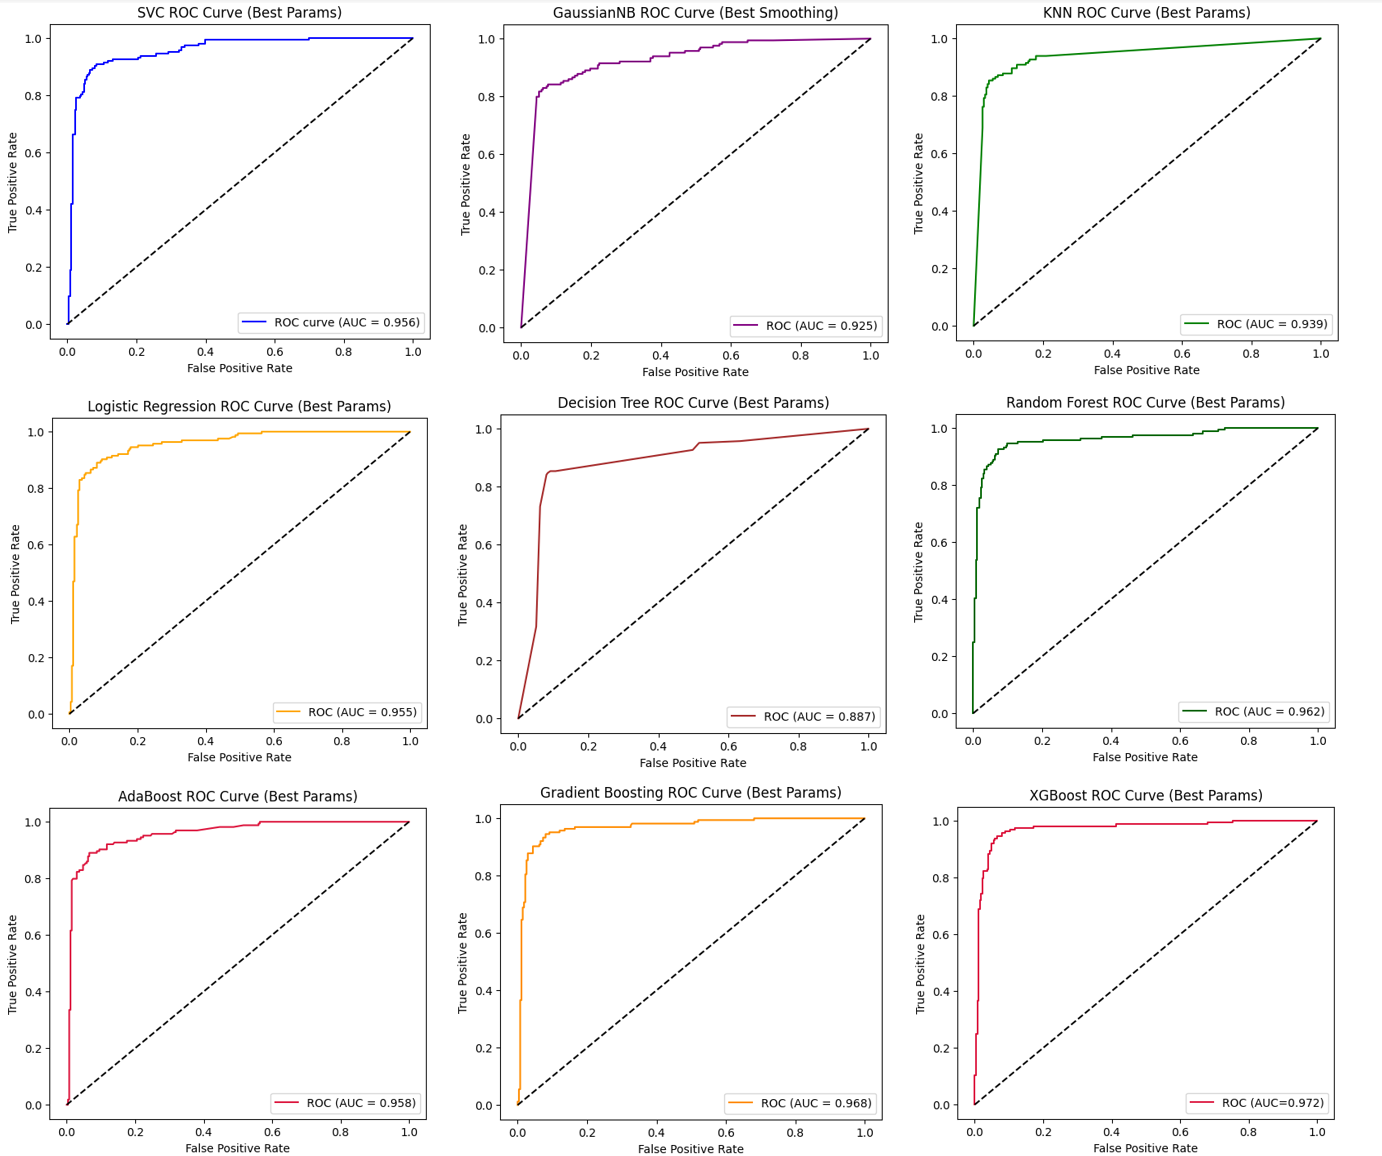
\includegraphics[width=0.9\textwidth]{expt6/expt-6_files/subplot.png} 
\caption{Plots comparison}
\end{figure}

\vspace{0.8cm}
\section{Hyperparameter Tuning Tables}
\vspace{0.5cm}
\textbf{PCA Summary}
\begin{table}[H]
\centering
\caption{Decision Tree - PCA Summary}
\begin{tabular}{|l|c|c|p{4cm}|} 
\hline
\textbf{Setting} & \textbf{Variance Target} & \textbf{Explained Variance (\%)} & \textbf{Justification} \\
\hline
With PCA & 95\% & 95.54 & Captures 95\% of total variance while reducing dimensionality, removing redundant features, and improving model efficiency. \\
\hline
\end{tabular}
\end{table}

\vspace{0.7cm}
\textbf{Support Vector Machine (SVM)}
\begin{table}[H]
\centering
\caption{SVM - Hyperparameter Tuning Results}
\begin{tabular}{|l|c|c|c|c|} 
\hline
\textbf{Kernel} & \textbf{C} & \textbf{Gamma} & \textbf{Performance (No-PCA)} & \textbf{Performance (With-PCA)} \\
\hline
linear & 0.1  & scale & 0.93135 & 0.924485 \\
linear & 10.0 & scale & 0.93135 & 0.924485 \\
rbf    & 0.1  & scale & 0.93135 & 0.924485 \\
rbf    & 10.0 & scale & 0.93135 & 0.924485 \\
\hline
\end{tabular}
\end{table}

\vspace{0.7cm}
\textbf{Naive Bayes}
\begin{table}[H]
\centering
\caption{Naive Bayes - Smoothing Choices}
\begin{tabular}{|c|c|c|} 
\hline
\textbf{Smoothing Parameter} & \textbf{Performance (No-PCA)} & \textbf{Performance (With-PCA)} \\
\hline
1e-09 & 0.720824 & 0.832952 \\
1e-08 & 0.723112 & 0.832952 \\
1e-07 & 0.725400 & 0.832952 \\
1e-06 & 0.725400 & 0.832952 \\
\hline
\end{tabular}
\end{table}

\vspace{0.6cm}
\textbf{K-Nearest Neighbors (KNN)}
\begin{table}[H]
\centering
\caption{KNN - Hyperparameter Tuning Results}
\begin{tabular}{|c|c|c|c|c|} 
\hline
\textbf{k} & \textbf{Weights} & \textbf{Metric} & \textbf{Performance (No-PCA)} & \textbf{Performance (With-PCA)} \\
\hline
3 & uniform  & euclidean & 0.899314 & 0.901602 \\
3 & distance & euclidean & 0.910755 & 0.908467 \\
3 & distance & manhattan & 0.903890 & 0.906178 \\
5 & distance & euclidean & 0.908467 & 0.910755 \\
\hline
\end{tabular}
\end{table}

\vspace{0.6cm}
\textbf{Logistic Regression}
\begin{table}[H]
\centering
\caption{Logistic Regression - Hyperparameter Tuning Results}
\begin{tabular}{|c|c|c|c|} 
\hline
\textbf{C} & \textbf{Penalty} & \textbf{Performance (No-PCA)} & \textbf{Performance (With-PCA)} \\
\hline
0.01 & l2 & 0.908467 & 0.908467 \\
0.01 & l1 & 0.871854 & 0.894737 \\
0.10 & l1 & 0.913043 & 0.917620 \\  
1.00 & l2 & 0.910755 & 0.901602 \\
\hline
\end{tabular}
\end{table}

\vspace{2.5cm}
\textbf{Decision Tree (DT)}
\begin{table}[H]
\centering
\caption{Decision Tree - Hyperparameter Tuning Results}
\begin{tabular}{|c|c|c|c|} 
\hline
\textbf{Criterion} & \textbf{Max Depth} & \textbf{Performance (No-PCA)} & \textbf{Performance (With-PCA)} \\
\hline
gini    & NaN  & 0.887872 & 0.883295 \\
gini    & 5    & 0.876430 & 0.860412 \\
gini    & 10   & 0.890160 & 0.874142 \\  % best params
entropy & 10   & 0.878719 & 0.878719 \\
\hline
\end{tabular}
\end{table}

\vspace{0.7cm}
\textbf{Random Forest}
\begin{table}[H]
\centering
\caption{Random Forest - Hyperparameter Tuning Results}
\begin{tabular}{|c|c|c|c|} 
\hline
\textbf{N Estimators} & \textbf{Max Depth} & \textbf{Performance (No-PCA)} & \textbf{Performance (With-PCA)} \\
\hline
50  & NaN  & 0.922197 & 0.906178 \\
50  & 5    & 0.910755 & 0.897025 \\
50  & 10   & 0.924485 & 0.908467 \\ 
100 & 10   & 0.922197 & 0.910755 \\
\hline
\end{tabular}
\end{table}

\vspace{0.7cm}
\textbf{AdaBoost}
\begin{table}[H]
\centering
\caption{AdaBoost - Hyperparameter Tuning Results}
\begin{tabular}{|c|c|c|c|} 
\hline
\textbf{N Estimators} & \textbf{Learning Rate} & \textbf{Performance (No-PCA)} & \textbf{Performance (With-PCA)} \\
\hline
50  & 0.01 & 0.821510 & 0.878719 \\
50  & 1.00 & 0.908467 & 0.892449 \\
100 & 0.10 & 0.899314 & 0.883295 \\
100 & 1.00 & 0.915332 & 0.901602 \\
\hline
\end{tabular}
\end{table}

\vspace{0.7cm}
\textbf{Gradient Boosting}
\begin{table}[H]
\centering
\caption{Gradient Boosting - Hyperparameter Tuning Results}
\begin{tabular}{|c|c|c|c|} 
\hline
\textbf{N Estimators} & \textbf{Learning Rate} & \textbf{Performance (No-PCA)} & \textbf{Performance (With-PCA)} \\
\hline
50  & 0.1 & 0.924485 & 0.901602 \\
50  & 0.2 & 0.922197 & 0.913043 \\
100 & 0.1 & 0.931350 & 0.908467 \\ 
100 & 0.2 & 0.929062 & 0.913043 \\
\hline
\end{tabular}
\end{table}

\vspace{2.5cm}
\textbf{XGBoost}
\begin{table}[H]
\centering
\caption{XGBoost - Hyperparameter Tuning Results}
\begin{tabular}{|c|c|c|c|c|} 
\hline
\textbf{N Estimators} & \textbf{Learning Rate} & \textbf{Max Depth} & \textbf{Performance (No-PCA)} & \textbf{With-PCA} \\
\hline
50  & 0.1 & 5 & 0.929062 & 0.908467 \\
50  & 0.2 & 7 & 0.938215 & 0.908467 \\
100 & 0.1 & 7 & 0.940503 & 0.910755 \\ % best params
100 & 0.2 & 7 & 0.933638 & 0.915332 \\
\hline
\end{tabular}
\end{table}

\vspace{1.2cm}
\textbf{Stacked Models}
\begin{table}[H]
\centering
\caption{Stacked Model Performance}
\begin{tabular}{|l|c|c|} 
\hline
\textbf{Model} & \textbf{Performance (No-PCA)} & \textbf{Performance (With-PCA)} \\
\hline
SVM+NB+DT $\rightarrow$ LR & 0.917620 & 0.913043 \\
SVM+NB+DT $\rightarrow$ RF & 0.892449 & 0.899314 \\
SVM+DT+KNN $\rightarrow$ LR & 0.919908 & 0.919908 \\
\hline
\end{tabular}
\end{table}

\vspace{1.8cm}
\textbf{5-Fold Cross-Validation Results}
\begin{table}[H]
\centering
\caption{5-Fold Cross-Validation Performance (No-PCA vs With-PCA)}
\begin{tabular}{|l|c|c|c|c|c|c|c|} 
\hline
\textbf{Model} & \textbf{Fold 1} & \textbf{Fold 2} & \textbf{Fold 3} & \textbf{Fold 4} & \textbf{Fold 5} & \textbf{Avg (No-PCA)} & \textbf{With-PCA} \\
\hline
XGBoost             & 0.9405 & 0.9268 & 0.9497 & 0.9519 & 0.9634 & 0.9465 & 0.9263 \\
Random Forest       & 0.9291 & 0.9108 & 0.9451 & 0.9405 & 0.9519 & 0.9355 & 0.9195 \\
Gradient Boosting   & 0.9199 & 0.9176 & 0.9451 & 0.9359 & 0.9519 & 0.9341 & 0.9227 \\
Stacked             & 0.9176 & 0.9108 & 0.9382 & 0.9336 & 0.9359 & 0.9272 & 0.9249 \\
AdaBoost            & 0.9085 & 0.9130 & 0.9291 & 0.9314 & 0.9291 & 0.9222 & 0.9085 \\
Logistic Regression & 0.9153 & 0.8947 & 0.9291 & 0.9336 & 0.9336 & 0.9213 & 0.9176 \\
SVM                 & 0.9153 & 0.9016 & 0.9268 & 0.9314 & 0.9222 & 0.9195 & 0.9236 \\
KNN                 & 0.9085 & 0.9016 & 0.9291 & 0.9108 & 0.8879 & 0.9076 & 0.9089 \\
Decision Tree       & 0.8970 & 0.8810 & 0.9176 & 0.9153 & 0.8810 & 0.8984 & 0.8838 \\
Naive Bayes         & 0.7323 & 0.7368 & 0.7506 & 0.7254 & 0.7735 & 0.7437 & 0.8384 \\
\hline
\end{tabular}
\end{table}

\vspace{3.0cm}
\textbf{Train vs Test Performance}
\begin{table}[H]
\centering
\caption{Train and Test Performance of Models}
\begin{tabular}{|l|c|c|} 
\hline
\textbf{Model} & \textbf{Train Performance} & \textbf{Test Performance} \\
\hline
XGBoost             & 0.9931 & 0.9405 \\
Gradient Boosting   & 0.9771 & 0.9314 \\
Random Forest       & 0.9760 & 0.9245 \\
Stacked             & 0.9811 & 0.9153 \\
AdaBoost            & 0.9394 & 0.9153 \\
Logistic Regression & 0.9308 & 0.9153 \\
KNN                 & 1.0000 & 0.9108 \\
SVM                 & 0.9331 & 0.9108 \\
Decision Tree       & 0.9725 & 0.8902 \\
Naive Bayes         & 0.7586 & 0.7254 \\
\hline
\end{tabular}
\end{table}

\vspace{0.5cm}
\section{Observations}
\begin{itemize}
    \item \textbf{Which models improved most with PCA? Which did not? Why?} \\
    Naive Bayes and KNN benefited most from PCA, with Naive Bayes rising from 0.7437 to 0.8384 and KNN from 0.9076 to 0.9089 in 5-fold CV. Ensemble models like Random Forest, Gradient Boosting, and XGBoost improved moderately (~0.5–0.7\%), showing PCA mainly aids models sensitive to correlated or redundant features.

    \item \textbf{Did PCA reduce variance across folds (more stable results)?} \\
    Yes. For most models, the fold-to-fold fluctuation decreased slightly with PCA. For example, Naive Bayes' standard deviation across folds dropped noticeably (from ~0.015 to ~0.007), indicating PCA stabilized learning by removing noisy/redundant features. 

    \item \textbf{For high-dimensional data, was PCA beneficial in reducing overfitting?} \\
    PCA helped reduce overfitting for simpler or more flexible models. Naive Bayes and KNN had better test performance after PCA, while ensemble models were already robust. 

    \item \textbf{How did linear models (Logistic Regression, SVM) behave compared to ensemble models with PCA?} \\
    SVM and Logistic Regression showed minor changes in both CV and test performance, suggesting linear models are less sensitive to redundant features in this dataset. In contrast, ensemble methods like Random Forest, Gradient Boosting, and XGBoost maintained high performance with PCA, confirming their inherent ability to handle high-dimensional input without heavy reliance on dimensionality reduction.  

    \item \textbf{Did stacking show robustness to dimensionality reduction compared to single models?} \\
    Yes. The Stacked Ensemble model retained its top performance with PCA (CV: 0.9272 → 0.9249, Test: 0.9199 → 0.9199), showing minimal drop. This indicates stacking aggregates the strengths of base learners and is robust to moderate feature reduction, outperforming most individual models even when dimensions are reduced.  
\end{itemize}

\vspace{1cm}
\section{Learning Outcomes}
\begin{itemize}
    \item Gained hands-on experience performing hyperparameter tuning for multiple classifiers including SVM, KNN, Naive Bayes, Logistic Regression, Decision Tree, Random Forest, AdaBoost, Gradient Boosting, and XGBoost.
    \item Learned to apply PCA for dimensionality reduction and observed its impact on model performance, variance, and overfitting.
    \item Understood how different models respond to PCA, identifying which models benefit most (Naive Bayes, KNN) and which are robust to high-dimensional data (ensemble methods, linear models).
    \item Observed how stacking ensembles can improve predictive performance and maintain robustness to dimensionality reduction compared to individual models.
\end{itemize}


\vspace{1cm}
\noindent
\textbf{GitHub Repository:} \\
\href{https://github.com/vidarshanaa15/ml-expt-6}{https://github.com/vidarshanaa15/ml-expt-6}
    
\end{document}
